%% Copernicus Publications Manuscript Preparation Template for LaTeX Submissions
%% ---------------------------------
%% This template should be used for copernicus.cls
%% The class file and some style files are bundled in the Copernicus Latex Package, which can be downloaded from the different journal webpages.
%% For further assistance please contact Copernicus Publications at: production@copernicus.org
%% https://publications.copernicus.org/for_authors/manuscript_preparation.html


%% Please use the following documentclass and journal abbreviations for discussion papers and final revised papers.

%% 2-column papers and discussion papers
\documentclass[hess, manuscript]{copernicus}
% Hydrology and Earth System Sciences (hess)

%% \usepackage commands included in the copernicus.cls:
%\usepackage[german, english]{babel}
%\usepackage{tabularx}
%\usepackage{cancel}
%\usepackage{multirow}
%\usepackage{supertabular}
%\usepackage{algorithmic}
%\usepackage{algorithm}
%\usepackage{amsthm}
%\usepackage{float}
%\usepackage{subfig}
%\usepackage{rotating}

\usepackage{siunitx}
\usepackage{subcaption}
\usepackage{amsmath}
\usepackage{amssymb}
% tables
\usepackage{booktabs}
\usepackage[normalem]{ulem}
\usepackage{multirow}
\useunder{\uline}{\ul}{}
%--------------------------------------------------------%
%	DOCUMENT
%--------------------------------------------------------%
\begin{document}
%--------------------------------------------------------%
\title{Estimating irrigation water use over the contiguous United States by combining satellite and reanalysis soil moisture data}
%--------------------------------------------------------%
% \Author[affil]{given_name}{surname}
\Author[1]{Felix}{Zaussinger}
\Author[1]{Wouter}{Dorigo}
\Author[1,3]{Alexander}{Gruber}
\Author[2]{Luca}{Brocca}
\Author[2]{Angelica}{Tarpanelli}
\Author[2]{Paolo}{Filippucci}
%--------------------------------------------------------%
%% The [] brackets identify the author with the corresponding affiliation. 1, 2, 3, etc. should be inserted.
\affil[1]{CLIMERS - Research Group Climate and Environmental Remote Sensing, Department of Geodesy and Geoinformation, TU Wien, Vienna, Austria}
\affil[2]{Research Institute for Geo-Hydrological Protection, National Research Council, Perugia, Italy}
\affil[3]{Department of Earth and Environmental Sciences, KU Leuven, Heverlee, Belgium}
%--------------------------------------------------------%
\runningtitle{Estimating irrigation water use over the contiguous United States by combining satellite and reanalysis soil moisture data}
\runningauthor{Felix Zaussinger}
\correspondence{Felix Zaussinger (felix.zaussinger@geo.tuwien.ac.at)}
%--------------------------------------------------------%
%% These dates will be inserted by Copernicus Publications during the typesetting process.
\received{}
\pubdiscuss{} %% only important for two-stage journals
\revised{}
\accepted{}
\published{}
%--------------------------------------------------------%
\firstpage{1}
\maketitle
%--------------------------------------------------------%
%	ABSTRACT
%--------------------------------------------------------%
\begin{abstract}
In many regions of the world, irrigation is indispensable for ensuring food-security. Irrigation significantly alters the hydrological cycle, as over 70\% of global freshwater is used for agriculture and acts as an important anthropogenic climate forcing through enhancing evaporation and therefore cooling the near land surface on local- to regional scales. Therefore, accurate and timely information on the extents and water consumption of existing irrigated areas and their development are needed for effective water management and improving land surface- and climate models. However, existing irrigation data often lacks the objectivity and spatial representativeness needed for such applications. While several studies have used optical remote sensing data to map irrigated areas, soil moisture (SM) data and in particular the derivation of irrigation water use has been less widely considered. Space borne sensors operating in the microwave range operationally observe the moisture in the top-most centimeters of soil, which is directly influenced by agricultural irrigation practices.\\

In this paper, we evaluate the potential of deriving actual irrigation water use (IWU) by combining SM data from three state-of-the-art passive (SMAP, AMSR2) and active (ASCAT) microwave sensors and reanalysis SM data (MERRA-2). Based on the assumption that neither the structure nor the forcing of the modelled data account for artificial water supply, while the remote sensing observations do, we develop a new methodology to estimate IWU at up to monthly time scales. The method is implemented in a contiguous US (CONUS) domain for the study period of 2013-2016. We find that state-aggregated IWU derived from SMAP shows good correlations with reported irrigation water withdrawals (r=0.79). In many regions, spatial irrigation patterns depict good agreements with the MIrAD-US data set on irrigated areas (e.g. producer's- and overall accuracies of 95.06\% and 77.68\% for SMAP over California). Particularly in semi-arid areas, where plants rely on full irrigation during the dry season, the observed seasonality is meaningful and exposes intra-annual variability of irrigation throughout the growing season. However, the results also show that the method significantly underestimates reported irrigation water withdrawals on the state level. We argue that this should be mainly attributed to the coarse spatial resolution ($\approx 40-km$) of the employed satellite SM data. To address these issues, the method should be further tested using higher resolution satellite SM data (e.g. SMAP enhanced 9-km, future Sentinel-1 SM products) and potentially extended with additional ancillary data (e.g. GRACE terrestrial water storage, vegetation data).
\end{abstract}
%--------------------------------------------------------%
%\copyrightstatement{...}
%--------------------------------------------------------%
%	1) Introduction
%--------------------------------------------------------%
\newpage
\introduction 
\label{sec:introduction}
%--------------------------------------------------------%
% 1) outline the general scientific area: Irrigation for food security, climate change
Over 70\% of global freshwater withdrawals are used for irrigation within the agricultural sector \citep{Shiklomanov2000, Foley2011}. Research shows that water will be a major constraint for agriculture in the coming decades, although expansion of irrigated areas will be necessary to increase food-security for a growing population and amplify economic development \citep{Rijsberman_2006}. Furthermore, climate change is will likely have a profound impact on irrigation demand throughout the world. Firstly, the projected mean increase in temperature and changing precipitation patterns are expected to decrease natural water availability in already water-scarce regions of the world \citep{Voeroesmarty2000,Rockstroem2012,Kummu2016}, resulting in increased irrigation water demand in the worlds food baskets \citep{Rijsberman_2006}. Secondly, it is expected that the hydrological cycle will intensify, enhancing the occurrence of drought and flood events which directly impact water availability for agriculture \citep{allan2008atmospheric}. For instance, it has been shown that around 2/3 of areas which were irrigated in 1995 will require more irrigation water by 2070 \citep{Doell2002}.\\

% impact of irrigation on climate change
Conversely, research shows that irrigation itself is an important anthropogenic climate forcing. Some authors argue that it might even be the human management practice with the overall biggest effect on climate \citep{sacks-2009}. Through increasing evapotranspiration, irrigation cools the land surface on local to regional scales, while the increased availability of atmospheric water vapor can enhance cloud cover and precipitation \citep{Boucher2004,lobell_2006, sacks-2009}. While there is general scientific agreement that the so called irrigation cooling effect (ICE) has a significant seasonal impact on near-surface temperatures in large regions of the world, the scale of the simulated cooling varies from negligible to $1.3 \si{\degree} C$ on a global scale and $\approx 0.5 K$ - $\approx 8 \si{\degree} C$ on a local to regional scale.
% implications
It is therefore crucial to consider the climatic feedback of irrigation both in terms of modeling future climate and understanding historical climate trends. Past expansion of irrigated areas and an overall increase in irrigation intensity may have significantly affected surface temperature observations and in turn potential evaporation on local to regional scales \citep{lobell_2006}. Assuming a similar future expansion of irrigation, some regions might actually benefit from these effects, as irrigation water requirements within agricultural micro-climates are reduced \citep{Ozdogan2006}. However, as irrigation may have masked the full warming signal caused by greenhouse gas emissions \citep{Bonfils2007, Kueppers2007} and future water availability is expected to decline in many heavily irrigated semi-arid regions of the world \citep{Rijsberman_2006}, a decrease in irrigation intensity yielding a coupled decrease in ICE could potentially amplify the warming signal and lead to more pronounced heat-waves which threaten food-security.\\

% Need for irrigation data, what are the applications
Consequently, accurate and timely information about the spatio-temporal distribution and development of irrigated areas and irrigation water use are crucial for a large number of stakeholders. Particularly in water-scarce regions, government agencies and water managers need to effectively monitor their efforts on increasing water use efficiencies, control the distribution of water among farms in a irrigation district and detect illegal groundwater pumping activities \citep{Siebert2010,taylor-2012}. The immanent importance of appropriate irrigation data for effective water management can already be observed in the California Central Valley, where a combination of prolonged winter precipitation deficits and positive temperature anomalies triggered a record breaking drought during 2012-2017. While farmers tried to compensate the 2015 surface water shortage ($-10.73 km^{3}$) by pumping more groundwater ($7.65 km^{3}$), a net water shortage of $3.08 km^{3}$ resulted in the fallowing of $\approx 228647.39 ha$ of land \citep{howitt2015}. From a research perspective, irrigation is an important variable in hydrological, climate and energy-budget modeling, but has long been ignored in operational products. Clearly, there is a strong need for future generations of land surface- and climate models to explicitly account for irrigation \citep{gibson2017case}.

% Limitations of inventories and GMIA
\subsection{Limitations of official irrigated area and water withdrawal statistics}
However, the available information on irrigated areas and particularly irrigation water use lacks the objectivity, spatial consistency and temporal resolution needed for the above-mentioned applications \citep{Deines2017}. On a local to regional scale, some irrigation districts conduct regular surveys, but the data is often not publicly available, lacks geo-referencing and is difficult to compare due to different sampling techniques. The elementary source of large scale irrigation data are national and sub-national statistical units, which routinely collect information on irrigated area (usually area equipped for irrigation AEI, in some cases also the area actually irrigated AAI in the year of the census \citep{siebert-2005}) and/or irrigation water withdrawals. The Global Map of Irrigation Areas (GMIA) was the first global-scale geospatial irrigated area dataset \citep{Doell2002, doll2002global} based on such statistics. Sub-national irrigation data from various sources (FAO, UN, World Bank, Agriculture Departments) and geospatial information on the location and extent of irrigation schemes (point-, polygon- and raster data, land cover maps and satellite imagery) were combined to map areas equipped for irrigation (AEI) and areas actually irrigated (AAI) at $0.5^{\circ}$ resolution around the year 2000. The resolution was improved to 5 min x 5 min, with the latest version being 5.0 \citep{siebert-2005, Siebert2007}. As the quality of the underlying data varies extensively among different world regions and countries \citep{siebert-2005}, the uncertainties propagate into the spatial map. Additional limitations are the coarse compilation cycle (which depends on the national compilation cycles), which does not allow to study the impact of climate variability and market conditions on irrigation. In summary, the main limitations of statistical inventories and derived products are:

\begin{enumerate}
\item The quality of the data varies significantly among countries \citep{Siebert2010}. While the data for the United States is considered to be of good quality, many developing countries lack the resources for comprehensive reporting. 
\item National statistics are usually valid for different years depending on each countries individual compilation cycle (every 5 years in case of the US).
\item Irrigated area estimates usually reflect areas equipped for irrigation, rather than areas actually irrigated. Depending on climatic and market conditions, farmers may decide to only cultivate and irrigate a portion of their fields.
\item Irrigation volume estimates reflect irrigation water withdrawals rather than actual irrigation water use, which can again differ depending on climatic variability.
\item Naturally, survey based statistics are only based on a sample of farms, which may or may not be representative.
\item The methods are unable to reflect water application from illegal groundwater pumping activities.
\end{enumerate}

\subsection{Remote sensing for irrigation mapping}
Remote sensing offers the potential to overcome the above-mentioned limitations, since it provides synoptic and timely information with respect to many geophysical variables which are either directly or indirectly influenced by irrigation. In the following paragraphs, we give an overview of remote sensing related studies in irrigation area and -water use mapping with regard to different sensor domains and spatio-temporal scales.

\subsubsection{Optical and thermal remote sensing}
Data acquired by optical sensors (AVHRR, MODIS, Landsat) were extensively used for identifying irrigated areas on local-, regional- and global scales. There is widespread agreement that vegetation indices such as the Normalized Difference Vegetation Index (NDVI), Enhanced Vegetation Index (EVI), Greenness Index (GI) and Vegetation Condition Index (VCI) are effective proxies for irrigation, because irrigated and non-irrigated cropland show different spectral responses during the peak growing season \citep{Ozdogan_2010_2}. A wide range of studies used these metrics to map annual irrigated areas and their changes through time, either in combination with statistical inventory data or without.\\

\textbf{Global scale}
% LULC maps
Several global land use land cover (LULC) mapping efforts identified various agricultural land cover classes, but only few delineated rainfed and irrigated croplands. For example, the USGS Global Land Cover Characteristics (GLCC) data set was derived from 1-km Advanced Very High Resolution Radiometer (AVHRR) sensor data and identified four types of irrigated croplands in the year 1992 \citep{loveland2000development}. However, the classification algorithms were not tailored to irrigated area mapping, resulting in low classification accuracies. Thus, major differences were found between the USGS map and country level reports of irrigated area, originating from both the uncertainties of the inventory data and technical limitations of the remote sensing datasets \citep{Voeroesmarty2000}.

Through a combination of unsupervised clustering and expert knowledge, the European Space Agency (ESA) produced a global land cover product valid for 2006 (GlobeCover) at 300m resolution using Medium Resolution Imaging Spectrometer (MERIS) data. More recently, a land cover product was developed within the ESA Climate Change Initiative (CCI) program \citep{bontemps2013consistent}. This product distinguishes irrigated and non-irrigated cropland for 2000, 2005 and 2010, but we argue that the irrigated class can not be considered reliable, as for instance no irrigated areas were mapped within the contiguous United States (CONUS).\\

% Tailored approaches for global maps
% MIRCA2000
Other studies used approaches specifically tailored to irrigated area mapping. For instance, the global data set of monthly irrigated and rainfed crop areas around the year 2000 (MIRCA2000) provides irrigated and rainfed areas for 26 crop classes for each month of the year at a spatial resolution of 5 arc min \citep{portmann2010mirca2000}. For this purpose, agricultural census statistics, national reports, databases, a map of crop specific annual harvested area, a cropland extent map, the GMIA, crop calendars and ancillary information on climate and topography were combined in a classification scheme.
% GIAM
Using quantitative spectral matching techniques on NDVI time series from multiple sensors (AVHRR, SPOT-1, MODIS and Landsat 7), JERS-1 SAR data over rain forests in combination with climate (monthly precipitation and temperature data from CRU) and ancillary data (GTOPO30 1km DEM, global tree cover), the International Water Management Institute (IMWI) produced a Global Irrigated Area Map (GIAM) at 1km resolution around the year 2000 \citep{Thenkabail2009}. 
% GRIPC
More recently, \citet{Salmon2015} created a global map of rain-fed, irrigated and paddy croplands (GRIPC) circa 2005 at 500m spatial resolution using supervised classification of remote sensing, climate, and agricultural inventory data.\\
% discrepancies among global datasets
However, there are large discrepancies between the different global datasets. For example, GRIPC estimated 314 Mha of global irrigated cropland, which agrees closely with national inventory statistics from FAOSTAT (305 Mha), but includes 24\% less area than the GIAM map (399 Mha) \citep{Salmon2015}. Moreover, three of the four existing global maps (GMIA, MIRCA2000 and GRIPC) rely on agricultural inventory data for the classification of irrigated areas, which as discussed is subject to major limitations concerning quality and accuracy. In addition, the maps are limited to single years (GMIA, GIAM, GRIPC), or single months within a single year (MIRCA2000), thus not being able to address the high inter-annual variability of irrigated areas, which is mainly governed by climate conditions and commodity prices \citep{Deines2017}.\\

\textbf{Continental scale}
On a continental scale, MODIS 250-m NDVI data found significant use. For instance, the MODIS Irrigated Agriculture Dataset for the conterminous United States (MIrAD-US) was created by assimilating county level irrigation statistics with MODIS derived seasonal peak NDVI to spatially identify irrigated and non-irrigated lands at 250-m resolution \citep{Ozdogan_2008, pervez2008evaluation, Pervez_2010}. A significant drawback is that the map compilation is tied to the same 5-year cycle of the USDS Census of Agriculture, preventing the study of inter-annual variability. \citet{Ambika2016} mapped irrigated areas from 2000–2015 at 250m resolution over India by using 250m MODIS seasonal peak NDVI data and 56m LULC data. For this purpose, a decision tree irrigation model \citep{Pervez2014,Pervez_2010} was adapted and Space Time Spiral Curves (ST-SCs) were used to separate irrigated and non-irrigated areas, with the advantage that no statistical inventory data was needed. \citet{Teluguntla2017} used spectral matching techniques (SMTs) and automated cropland classification algorithms (ACCAs) to infer cropland extent, irrigated versus rainfed croplands and cropping intensities over Australia. Thus, the latter two product allow to study inter-annual variability of irrigated areas on a continental scale, for instance the impact of drought on the fallowing of land \citep{Ambika2016}.\\

\textbf{Local to regional scale}
On a regional scale, higher resolution Landsat imagery was adopted by a range of studies. \citet{Ozdogan2006} used 30m Landsat imagery to map changes in annual irrigated area from 1993 to 2002 in southeastern Turkey based on NDVI thresholding approaches and compared them with $ET_{P}$ estimates on irrigation water requirements. Based on these estimates, irrigated area in this region has increased by $\approx 300\%$ and agricultural water use has roughly tripled. In a recent study, \citet{Deines2017} produced annual irrigation maps for 1999-2016 for a region in the High Plains Aquifer (United States) at 30m resolution and found considerable inter-annual variability in irrigation location and extent. In a similar study domain, \citet{Pun2017} used surface energy balance (SEB) partitioning and vegetation indices to classify irrigated and non-irrigated croplands at 30m resolution in Nebraska.
%TODO: Sentinel 1 and 2 \citep{Ferrant2017}
%TODO: Irrigation water use mapping (proxies: evaporation, heat fluxes, energy balance, ETp, ETo, crop factor; methods: SEBAL, SEB ...)
\subsubsection{Microwave remote sensing}
When farmers apply irrigation water to their field, this directly increases soil moisture. Because dry and wet soils exhibit a large difference between dielectric constants, space-born sensors operating in the microwave spectrum can be used to estimate soil moisture \citep{wagner2013ascat,wagner1999method,entekhabi2010soil}. However, remotely sensed soil moisture data received little attention for mapping irrigated areas and agricultural water use, a fact that was specifically addressed in \citet{Ozdogan_2010_2}, who argued that this area should be further researched. Potential advantages of these data are the high temporal resolution combined with the ability to sense through dense cloud cover, and the intrinsic capacity to sense a geophysical variable which is very directly and physically linked to irrigation. These characteristics could provide both stand-alone and synergistic value together with higher spatial resolution optical data, as the coarse spatial resolution ($\approx 25 - 50 km$) of most operational soil moisture products (e.g. SMAP, SMOS, AMSR2 and ASCAT) is an obvious drawback. However, the usefulness of these data for irrigation monitoring will likely increase as higher resolution products (e.g. SMAP enhanced 9km, Sentinel-1) \citep{Hornacek2012} and downscaling algorithms \citep{escorihuela2016comparison} are becoming available.\\

The first study to investigate the utility of satellite soil moisture retrievals for irrigation monitoring was carried out by \citet{Kumar_2015}, who used data from ASCAT, AMSR-E, SMOS, ESA-CCI SM and Windsat together with modeled SM estimates (NOAH) to map irrigated areas in a continental US domain. The key assumption was that irrigation is not included in the formulation of the land surface model (LSM), while satellite derived SM data is expected to reflect the wetter soil conditions induced by seasonal irrigation. While based on synthetic data the employed Kolmogorov-Smirnov test was able to detect differences between the probability density functions (PDF's) of satellite and model soil moisture data, the use of actual satellite-derived data showed only few systematic differences that could be reliably related to irrigation practices. The authors highlighted that the differences in the land surface parametrization of the respective models likely dominated the remotely sensed irrigation signal and that the scale mismatches between model and the satellite observations further deteriorated the results.\\

Satellite SM data also has the potential to improve predictions of crop yield and irrigation demand in agricultural models at field and regional scales \citep{ElSharif2015}. Medium- to high resolution soil moisture data (SMAP 9km, Sentinel-1) would be particularly useful to reduce numerical model uncertainties in regions where observed weather or soil moisture data are sparse or unavailable. \citet{Qiu2016} compared trends from the microwave based
multi-satellite surface soil moisture product (ESA CCI), ERA Interim/Land
reanalysis, and in-situ measurements and precipitation from 1996–2010 in China. Significant discrepancies between precipitation and soil moisture data sets were observed over major irrigation regions in the southwest and north of China, particularly in the Huang-Huai-Hai Plain. The authors argued that the impact of irrigation needs to be considered when assimilating microwave-based soil moisture into models. \citet{escorihuela2016comparison} compared three global soil moisture products (ASCAT, AMSR and SMOS) with model soil moisture estimates in a Mediterranean landscape. It was expected that correlation between satellite and model soil moisture is low over a heavily irrigated area, because the model does not take irrigation into account, but only SMOS soil moisture, in particular a downscaled version (SMOScat), was able to detect the seasonal irrigation. The authors argue that primarily due to the coarse spatial resolution, the other sensors were not able to resolve the irrigation in the mixture of the soil moisture signal from the irrigated pixel and of the surrounding dry-land area. Very recently, \citet{Lawston2017} investigated the potential of the new SMAP enhanced 9km soil moisture product to identify irrigation signals in three semi-arid regions in the western United States. Results showed that SMAP clearly detects irrigation signals from rice irrigation in the Sacramento Valley (California), while the signals were less significant in the other two regions.

\subsubsection{Representation of irrigation in land surface-, weather- and climate-models}
To date, agricultural land use is not explicitly represented in land surface models (LSMs), data assimilation systems and climate model simulations. Nonetheless, irrigation directly affects land surface temperature-, surface humidity- and soil moisture-observations, which when assimilated into models have considerable local- to regional scale impact. For instance, \citet{Wei_2013} showed that irrigation substantially contributes to precipitation in the MERRA land surface model over heavily irrigated regions in Asia. More recently, \citet{Tuinenburg2017} revealed that irrigation resembles soil moisture additions in the ERA‐Interim reanalysis soil moisture data and advocated the need to explicitly include irrigation in reanalysis models.\\ 

The assimilation of satellite-derived irrigation data could largely improve the representation of land-atmosphere feedbacks in land surface models, weather forecast, as well as climate fore- and hindcasts. In this scope, \citet{Ozdogan_2010} proposed a method which integrates satellite-derived irrigated area data into a land surface model by applying a demand driven sprinkler irrigation scheme (water application is triggered at irrigated cells when root zone soil moisture falls below a prescribed threshold). It was shown that irrigation significantly influences the surface water and energy balances over the continental United States, by modulating the partitioning of water between the surface and the atmosphere. However, data on actual irrigation water use is needed, because the irrigation algorithms in many modeling studies may not accurately represent actual on-farm practices (fields are over- or under-irrigated) and the true spatio-temporal variability of irrigation driven by climate and market conditions. The fact that the simulated impact of irrigation on climate shows considerable variation should also be primarily explained by the difference in the underlying irrigation algorithms which control the application of irrigation water \citep{sacks-2009}.\\

% 2) introduce specific part investigated in the manuscript
In summary, a wide range of studies investigated irrigated area mapping at various spatial (global, regional and local) and temporal (multi-year, annual and monthly) scales using remotely sensed data in the optical domain in combination with crop inventory and climate data. Concerning irrigation water volumes, surface energy balance methods exploiting remotely sensed land surface temperature have been used to map irrigation water requirements based on evaporation on local to regional scales. In the microwave domain, recent studies started to investigate the potential of remotely sensed soil moisture for detecting irrigation signals. However, to date no attempt was made to derive actual irrigation water use, as opposed to irrigation water requirements.
% 3) pose research question and briefly outline results and discussion
This study tries to meet the increasing need for independent and consistent information on agricultural land use by presenting a new method for estimating irrigation water use from a combination of remotely sensed and reanalysis soil moisture (SM) data. Based on the hypothesis that neither the structure nor the forcing of the modeled data account for artificial water supply, while the microwave SM retrievals sense the soil wetting through irrigation \citep{Kumar_2015, escorihuela2016comparison}, spatial irrigation patterns and seasonal irrigation water use are derived from differences between the modeled and remotely sensed SM climatology during the growing season. The method is implemented over the continental United States by using 3 state-of-the-art microwave SM products (SMAP, AMSR2 and ASCAT) in combination with MERRA-2 reanalysis SM and tested for the time period of 2013-2016.\\

% Paper structure
The paper is organized as follows: section \ref{sec:background} gives an overview of the general irrigation landscape in the contiguous United States (CONUS), focusing on the distribution of irrigated areas, irrigation water withdrawals and -practices. Data sets are explained in section \ref{sec:data} and the methodology is illustrated in section\ref{sec:methods}. Results are shown and discussed in section \ref{sec:results-and-discussion}. Lastly, conclusions are drawn in section \ref{sec:conclusions} and an outlook is given.

%--------------------------------------------------------%
%	2) Irrigation in the contiguous United States (CONUS)
%--------------------------------------------------------%
\newpage
\section{Irrigation in the contiguous United States (CONUS)}
\label{sec:background}
%--------------------------------------------------------%
The amount of water needed by a certain crop for optimal growth mainly depends on 3 factors: crop type, soil and climate. In turn, these factors determine the irrigation water need, which is defined as the difference between crop water requirements and effective rainfall. In the semi-humid climate of the eastern United States, irrigation is usually supplemental (SI), which means that irrigation is applied to essentially rainfed crops during times of insufficient rainfall and aims at achieving higher yield levels than under rain-fed-only conditions. In contrast, the predominantly semi-arid climate of the western US makes artificial water supply a necessity, thus requiring full irrigation (FI). Here, the most important source of moisture is irrigation water, which is supplemented by limited amounts of rainfall. In the scope of this study, it is important to understand how irrigation influences soil moisture variability both spatially and temporally. Therefore, this section gives a short overview of irrigation practices throughout the contiguous US and presents an extract of the latest inventory data on irrigation areas, -water withdrawals and -techniques.\\

The National Agricultural Statistics Service (NASS) of the U.S. Department of Agriculture (USDA) compiles a comprehensive summary of agricultural activity for the whole country and for each state in a 5-year cycle. The last \glqq Census of Agriculture\grqq \citep{nass2012census} is available for 2012. As a supplement to the census program, the 2013 Farm and Ranch Irrigation Survey (FRIS) \citep{fris2013} provides selected irrigation data for on-farm irrigation operations which was drawn from surveys conducted at $\approx 35000$ farms using irrigation across the US. The FRIS reports both irrigated area and irrigation water withdrawal statistics by specific crop type, water source and irrigation technique on the state level. In addition, estimates are further subdivided for crops cultivated in the open and under protection (e.g. horticultural crops grown in greenhouses). In the scope of this study, this information is important because it is expected that the irrigation water applied to crops grown under protection does not affect the remotely sensed soil moisture signal and we thus cannot observe these amounts. Consequently, figure~\ref{fig:background-irrigation-area-volumes} shows the per state irrigated area and irrigation water withdrawals limited to crops grown in the open during the 2013 growing season.\\ 

% HOW can i say this when i do not present results in these units?
Depending on climate, high shares of  state-aggregated irrigated area are not necessarily related to high irrigation water use. Therefore, the measure we are interested in is irrigation water applied per unit area. Figure~\ref{fig:background-irrigation-application-rates} depicts the state wise distribution of water application rates in total and subdivided for the main irrigation systems. We expect that among other factors, the sensitivity of the SM retrievals to irrigation increases as the irrigation application efficiency decreases and expect higher sensitivity towards gravity-, yet lower sensitivities towards sprinkler- and micro-irrigation systems. The data reveals a distinct decline in irrigation per area from the semi-arid west to the more humid east. The state of Arizona ranks highest, followed by California and Nevada. Gravity flow systems show the highest rates in California and Arizona, but also depict large values along the Mississippi Delta. This can be attributed to the cultivation of rice which is primarily grown in these regions and either flood or furrow irrigated. Finally, micro-irrigation systems are largely limited to the western half of the US.

%--------------------------------------------------------%
%	3) Data sources
%--------------------------------------------------------%
\newpage
\section{Data sources}
\label{sec:data}
The data sources used in this study area summarized in table~\ref{table:data-products}. In the following, a brief overview of the satellite and reanalysis SM products as well as of the ancillary data is given. 
%--------------------------------------------------------%
\subsection{Remotely Sensed Soil Moisture}
\textbf{SMAP} 
The Soil Moisture Active Passive (SMAP) mission was launched in January 2015 and is the second platform exclusively designed for the retrieval of surface soil moisture (SM) together with freeze-/thaw status \citep{entekhabi2010soil}. SMAP initially carried both an L-band radar ($1.26 GHz$) and radiometer ($1.41 GHz$), with the overall goal of combining the high spatial resolution of the radar with the high accuracy of the radiometer. Unfortunately, the radar failed functioning in July 2015 due to an instrument anomaly, but the radiometer continues to provide high quality SM estimates at $\approx 40-km$ spatial resolution. Preliminary validation studies show that the mission target accuracy of $4\%$ volumetric accuracy is met \citep{colliander2017validation}. In general, L-band is expected to be most suitable for SM retrieval, because at these wavelengths the atmosphere is more opaque, the retrievals are less affected by vegetation and representative of a deeper soil layer (e.g. the topmost $\approx 5-cm$ of soil, as compared to $\approx 2.5-cm$ at C-band) \citep{entekhabi2010soil}. Global coverage is archived every 2-3 days with a swath width of $\approx 1000 km$ and equatorial crossing times of 06:00 LST for the descending and 18:00 LST for the ascending orbit. We used data from both ascending and descending orbits of the passive SMAP\_L3\_v4 product from April 2015 to December 2016. In case of overlapping orbits, the descending overpass was used.\\ 

\textbf{AMSR2 (VUA-NASA product)}
AMSR2 is a microwave radiometer on board the GCOM-W1 satellite and provides passive microwave measurements representative of the first $\approx 1-cm$ of soil at 6.9 GHz (C-band) and three higher frequencies up to $36.5 GHz$ (Ka-band) since July 2012 \citep{Imaoka2010}. Daily ascending and descending overpasses are at 13:30 LST and 01:30 LST respectively and have a swath-width of 1450 km, archiving global coverage in 1-2 days. Within the VUA-NASA algorithm, volumetric soil moisture (\si{\m^{3}.\m^{-3}}) and vegetation optical depth (VOD) are simultaneously retrieved by applying the Land Parameter Retrieval Model \citep{Owe2008} (in this case LPRM version 6) to the observed brightness temperatures. The model is based on a simple radiative transfer equation and partitions the observation into it's emission components from soil and vegetation based on the horizontal and vertical polarized brightness temperatures. The data was masked for high VOD values and radio frequency interference (RFI), spatially resampled to a regular $0.25 \si{\degree}$ grid and temporally centered at 12:00 UTC.\\

\textbf{ASCAT}
The Advanced Scatterometer (ASCAT) on board the Meteorological Operational (METOP) satellites is operational since October 2006 and is a real aperture radar instrument operating at C-band ($5.255 GHz$) and VV polarization. Local equatorial crossing times (LST) are at 21:30 for the ascending overpass and at 09:30 for the descending overpass and global coverage is archived in 1-3 days depending on latitude. The TU Wien change detection algorithm \citep{wagner1999method, naeimi2009improved} is applied to the backscatter coefficients to create time series of relative surface SM for the topmost centimeters ($< 2-cm$) of soil. This is accomplished by scaling each observation between reference values which respectively represent the historically lowest and highest observed backscatter value. The SM data is provided in degrees of saturation (\%), hence ranging between 0\% (wilting point) and 100\% (saturation), has a spatial resolution of 25-km and made available on a discrete global grid (DGG) at a spatial sampling of 12.5-km. In this study, we employed a modified version of the H SAF (EUMETSAT Satellite Application Facility on Support to Operational Hydrology and Water Management) H111 soil moisture product. Like H111, the modified version includes both ascending and descending orbits but in contrast to the climatological vegetation correction of H111, it uses a dynamic correction which is expected to better account for inter-annual variability \citep{Hahn2017,Vreugdenhil2016}.

\subsection{MERRA-2 reanalysis soil moisture}
The second Modern-Era Retrospective analysis for Research and Applications 2
(MERRA-2) \citep{bosilovich2015merra} is an atmospheric reanalysis product which provides global, 1-hourly fields of land surface and atmospheric conditions for 1980-present at $\approx 50-km$ resolution and a spatial sampling of $0.625 \si{\degree}$ x $0.5 \si{\degree}$. In contrast to its predecessor MERRA, it uses an upgraded version of the Goddard Earth Observing System Model (GEOS-5) data assimilation system which enables the incorporation of new satellite instruments into the assimilation scheme (e.g. modern hyperspectral radiance and microwave observations together with GPS-Radio Occultation data sets) as older instruments fail. In contrast to MERRA, MERRA-2 uses an observation based precipitation correction over land which significantly improved the SM simulations. For this purpose, CPC Unified Gauge-Based Analysis of Global Daily Precipitation \citep{Xie2010} at $0.5\si{\degree}$ is used to fully correct modeled precipitation at $|lat|<42.5$, with a linear tapering between $42.5° < |lat| < 62.5°$ (no correction is applied at more northern latitudes). The SM simulations are representative of the first 10-cm of soil and expressed in volumetric units (\si{\m^{3}.\m^{-3}}). We explicitly chose MERRA-2 in favour of other global reanalysis data sets (e.g. ERA-Interim/Land, GLDAS) because surface humidities and temperature observations, which are affected by irrigation \citep{Wei_2013, Tuinenburg2017}, are not assimilated. 

\subsection{Ancillary data}
The ESA-Climate Change Initiative (CCI) Land Cover data set \citep{bontemps2013consistent} was used to create a cropland mask for the CONUS. The cropland classes of the data set representative of the period 2008-2012 were spatially aggregated to match the 0.25\si{\degree} target resolution of the common data grid. The spatial analysis was then restricted to pixels with $\geq 5\%$ fractional cropland area. Additional precipitation data was employed within the methodology. For this purpose, we used CPC Unified Gauge-Based Analysis of Daily Precipitation, which covers the CONUS at 0.25\si{\degree} native resolution \citep{Chen2008, Xie2010}. The MODIS Irrigated Agriculture data set for the conterminous United States (MIrAD-US) \citep{Pervez_2010} was used to evaluate the spatial patterns of the obtained results. This binary classification of irrigated areas at 250-m native resolution was created by combining state-level irrigation statistics drawn from the United States Department of Agriculture \citep{nass2012census} and MODIS NDVI time series. In conjunction with the USDA national census report, the map is deployed in a 5-year cycle and currently available for the years 2002, 2007 and 2012. Although the authors denote that this product has not been thoroughly validated itself and should be used with caution, it is currently considered as the state-of-the-art product for the continental United States, since it is closely tied to the official USDA irrigation statistics. The 2012 MIrAD-US was spatially aggregated to 0.25\si{\degree} resolution, thus yielding irrigated area from 0-100\%.

%--------------------------------------------------------%
%	4) Methods
%--------------------------------------------------------%
\newpage
\section{Methods}
\label{sec:methods}
%--------------------------------------------------------%
In this study, we present a new method for estimating irrigation water use (IWU) by combining remotely sensed and modeled SM data. \citet{Kumar_2015} first proposed the idea that irrigation can be inferred from a (positive) bias between remotely sensed and modeled SM, which is induced by seasonal water application during the dry season. This approach is based on two key assumptions: firstly, that the satellite SM products are indeed sensitive to large scale irrigation (as partly confirmed by \citet{escorihuela2016comparison, Lawston2017}) and secondly, that the model does not explicitly account for irrigation (e.g. in the formulation) nor implicitly through the assimilation of surface humidity or surface temperature observations, which are affected by irrigation \citep{Wei_2013}. Based on these assumptions, we introduce a new metric with the overall goal of estimating IWU at up to monthly time scales. We assume that changes in the water balance of the modeled SM are only driven by natural processes, whereas irrigation directly affects the soil moisture conditions observed from space born microwave remote sensing systems. The soil water balance equations that describe the variations in remotely sensed and modeled SM can then be respectively described by:
%
\begin{equation}
\label{eq:waterbalance}
\begin{gathered}
P + I = ET + R + \frac{d\Theta_{sat}}{dt} + \Delta S_{rest} \\
P = ET + R + \frac{d\Theta_{mod}}{dt} + \Delta S_{rest}
\end{gathered}
\end{equation}
%
where $P (\si{\mm})$ is precipitation, $I (\si{\mm})$ is irrigation, $ET (\si{\mm.\day^{-1}})$ is evapotranspiration, $\Theta_{sat}$ and $\Theta_{mod} (\si{\m^{3}.\m^{-3}})$ are satellite and modeled surface SM and $\Delta S_{rest} (\si{\m^{3}.\m^{-3}})$ describes water storage changes below the surface layer, including drainage. Subtracting the two equations yields:
%
\begin{equation}
\label{eq:irrigation-theoretical}
I =\frac{d\Theta_{sat}}{d t} - \frac{d\Theta_{mod}}{d t}
\end{equation}
%
Hence, estimating irrigation from differences between the temporal variations of satellite and model soil moisture is theoretically feasible. 

%--------------------------------------------------------%
\subsection{Pre-processing}
%--------------------------------------------------------%
Concerning the real world application, difficulties arise as the spatial representativeness and observation depths vary between remotely sensed SM and model SM, as well as amongst the individual SM retrievals. SMAP, AMSR2 and ASCAT microwave SM retrievals are provided in different units (volumetric and relative SM) and are representative of slightly different observation depths ($\approx$ 5-cm, $\approx$ 1-cm and $\approx$ 2.5-cm) which mainly depends on wavelength, soil wetness and vegetation cover. In contrast, MERRA-2 SM is simulated for a 10-cm thick soil layer \citep{bosilovich2015merra} and thus shows more inertia to changes in the water balance (i.e. through precipitation). These discrepancies introduce systematic differences between the remotely sensed and modeled SM data, which are accounted for by applying a linear rescaling approach \citep{draper2009evaluation,brocca2010spatial,brocca2013scaling} to the time series. Specifically, the satellite SM time series $ts_{sat}$ are forced to have the same mean $\mu$ and standard deviation $\sigma$ of the model SM time series $ts_{model}$:
%
\begin{equation} 
\label{eq:scaling}
ts_{sat_{rescaled}} = \frac{ts_{sat} - \mu(ts_{sat})}{\sigma(ts_{sat})} \sigma(ts_{model}) + \mu(ts_{model})
\end{equation}
%
\textbf{Unit conversion}
By now, all SM products are given in volumetric units ($\si{\m^{3}.\m^{-3}}$) and their temporal dynamics are assumed to be representative of the first 10-cm of soil. Since the variable of interest are irrigation amounts, volumetric SM in $(\si{\m^{3}.\m^{-3}})$ is converted to the corresponding water table depth $D_{watertable} (\si{\mm})$ by multiplying with the depth of soil $D_{soil}$. Thus, at a layer depth of 10-cm, $1~\si{\m^{3}.\m^{-3}}$ corresponds to a 100-mm deep water table covering the unit area of $1~\si{\m^{2}}$.\\

\textbf{Filtering and noise removal}
It is essential to differentiate between the irrigation signal entailed in the SM data over irrigated areas and high frequency noise. With the goal of reducing noise, three filtering techniques were tested: the moving average filter \citep{brocca2013scaling}, the Savitzky-Golay filter \citep{savitzky1964smoothing} and lastly the exponential filter \citep{wagner1999method,Albergel2008}. We found that among the filtering techniques, the exponential filter is the most appropriate choice for this application. Here, an asymmetrical window function is used which better preserves the temporal evolution of the soil moisture wetting (induced by rainfall or irrigation) and dry-down cycles. However, a sensitivity analysis (see section~\ref{ssec:sensitivity-analysis}, table~\ref{table:method-evaluation} for details) revealed that the use of the exponential filter resulted in poor agreements with the available reference data. Therefore, we chose to instead differentiate between noise and irrigation by applying thresholds to the relative soil moisture increases similar to \citet{dorigo2013global}. Based on the analysis we concluded that a relative threshold of 12\% is an appropriate choice, which corresponds to three times the SMAP mission target accuracy of $0.04~\si{\m^{3}.\m^{-3}}$ \citep{entekhabi2010soil}.

%--------------------------------------------------------%
\subsection{Deriving irrigation water use}
%--------------------------------------------------------%
In the following step, changes in satellite and model SM are determined by calculating  the difference quotients at each day of the growing season. In terms of growing season, an examination of the crop calendars provided by \citet{portmann2010mirca2000} and the USDA Planting and harvesting dates handbook \citep{nass2010usual} revealed that April-September is a reasonable generic choice for the CONUS, as it covers the growing seasons of most crops which receive irrigation. We define an irrigation event as a simultaneous increase in satellite SM ($\frac{d\Theta^{sat}}{dt} > 0$) and a decrease or stagnation in model SM ($\frac{d\Theta^{mod}}{dt} \leq 0$). This means that rainfall did not cause the observed increase in SM and thus over agricultural land was very likely a result of irrigation. For each event, the amount of irrigation water that lead to this increase is derived as the difference between $\frac{d\Theta^{sat}}{dt}$ and $\frac{d\Theta^{mod}}{dt}$. Seasonal irrigation water use (IWU) is then determined by summation over the growing season (GWS) period:
%
%\begin{equation}
\begin{gather}
\label{eq:irrigation}
IWU(i) = \sum_{i=SOS}^{EOS} \Delta d\Theta^{+}_{i}
%
\intertext{where}
\Delta d\Theta^{+}_{i} = \begin{cases} \Delta d\Theta^{}_{i}
, &\mbox{if } \Delta d\Theta^{}_{i} > 0 \nonumber \\ 
0, & \mbox{otherwise } \end{cases}
%
\intertext{and}
\Delta d\Theta^{}_{i} = \begin{cases}  d\Theta^{sat}_{i} - d\Theta^{mod}_{i}
, &\mbox{if } d\Theta^{sat}_{i} \geq \Theta_{thresh} \nonumber \\ 
0, & \mbox{otherwise } \end{cases}
%
\intertext{with}
d\Theta^{sat}_{i} = \Theta^{sat}_{i} - \Theta^{sat}_{i-t} \text{, } \nonumber \\
d\Theta^{mod}_{i} = \Theta^{mod}_{i} - \Theta^{mod}_{i-t} \nonumber
%
\end{gather}
%\end{equation}
% 
where $IWU(i)$ is the accumulated irrigation water use from the start ($SOS$) until the end of the growing season ($EOS$). $\Theta^{sat}_{i}$ and $\Theta^{mod}_{i}$ are satellite and model SM at day $i$, while $\Theta^{sat}_{i-t}$ and $\Theta^{mod}_{i-t}$ are the last available estimates with a data gap of $t$ days. The threshold variable $\Theta_{thresh}$ is used to constrain the summation to significant SM increases which are assumed to be caused by irrigation and aims at excluding spurious events caused by noise. Data gaps in the remotely sensed SM observations are treated in such a way that if an irrigation event is detected during an observation gap of $>4$ days, we check if there was a significant increase in the model SM time series (e.g. rainfall) within that period and disregard the potential irrigation event if there was at least one significantly positive model slope.\\

% Additional precipitation masking, capillary rise
However, potential errors arise when the model forcing misses or creates false rainfall events. In addition, it was found that the reaction of remotely sensed and modeled SM to precipitation events can differ. We therefore used CPC precipitation data to double check if the model forcing missed a rainfall event and prevent errors due to temporal mismatches in the response to precipitation (see section~\ref{ssec:sensitivity-analysis}, table~\ref{table:method-evaluation} for details). Furthermore, if we see a potential irrigation signal and it significantly rained the day before (as inferred from the model slope), we assume that irrigation is unlikely and disregard the event. Another potential difficulty is that in some extreme cases, capillary rise from deeper soil layers or run-on can potentially create soil wetting which is observed by the satellite SM data, but absent in the model data, if such effects are not accounted for in the soil hydrology formulation of the LSM. However, at the large spatial scale represented by the used satellite ($\approx 40 km$) and model soil moisture products ($\approx 50 km$), very few pixels are expected to show positive $d\Theta^{sat}_{i}$ or $d\Theta^{mod}_{i}$ in the absence of precipitation or irrigation.

% Normalization: Every pixel is associated with a specific crop fraction, which is derived from the CCI Land Cover product. Since the irrigation signal in the remotely sensed SM retrievals originates from the irrigated parts of the total cropland area, irrigation application rates $[m^3 ha^-1 yr^-1]$ can be obtained by normalizing the water table depth expressed in $m^3$ ($1000mm = 1 m^3$) with the agricultural area in $ha$.
%--------------------------------------------------------%
\subsection{Method implementation and study areas}
%--------------------------------------------------------%
% data sources, study domain, time period, resolution
% land-cover and sat ts masking
The method was implemented over the contiguous United States (CONUS) using remotely sensed SM from SMAP, AMSR2 and ASCAT in combination with MERRA-2 reanalysis soil moisture. While data from SMAP only was available from 2015/04 onwards, we extended the study period to use AMSR2 and ASCAT data from 2013 to 2016. Hence, 4 growing seasons with varying climatic conditions were covered by the AMSR2 and ASCAT sensors, while the most recently launched SMAP mission provided data for 2 seasons. As described, we assumed a generic and static growing season for the whole study area from April to September. The data were spatially matched to a common 0.25\si{\degree} regular grid using nearest neighbor search. In order to constrain the analysis to areas where irrigation is feasible, we masked all pixels with $<5\%$ of fractional cropland area based on the CCI land cover product for 2010 \citep{bontemps2013consistent}. Unreliable observations in the satellite soil moisture time series where masked using the respective quality flags. In addition to the continental-scale analysis, we chose 4 irrigation hotspots characterized by different climates and irrigation practices within the CONUS (figure~\ref{fig:study-areas-over-mirad}) to comprehensively assess the spatio-temporal dynamics of estimated IWU. The regions are: the Sacramento Valley (SV) and San Joaquin Valley (SJV), California; the Snake River Plain (SRP), Idaho; the Nebraska Plains (NP) and a part of the Mississippi Flood Plain (MFP) within the state of Mississippi. For each region, we conducted both a local time series analysis and a regional scale analysis of state-aggregated IWU.
%--------------------------------------------------------%
%	5) Results
%	- What did i observe and measure and what did i find out?
%	- Provide enough info to understand the interpretation of each 'experiment'
%	- 1 paragraph per experiment: aim, outcome, where to look at (figs, tables)
%--------------------------------------------------------%
\newpage
\section{Results and Discussion}
\label{sec:results-and-discussion}
%--------------------------------------------------------%
\subsection{Growing season correlations between satellite and model soil moisture}
\label{ssec:correlations}
%--------------------------------------------------------%
It was previously shown that over irrigated areas, systematic differences between remotely sensed and model SM estimates are mainly composed of a seasonal bias induced by the application of irrigation water, which is only observed by space-born microwave sensors \citep{Kumar_2015,escorihuela2016comparison}. Thus, similar to \citet{escorihuela2016comparison}, who found low correlations between a downscaled SMOS SM product and simulated SM over an intensively irrigated area, we expected a decrease in correlation between each satellite SM product and MERRA-2 SM during the growing season. To investigate if SM indeed deviates over such areas within the CONUS, the growing season correlations (Pearson's r) between the daily time series of each satellite SM product with MERRA-2 SM was computed for each year of the study period. We then calculated the mean of the respective growing season correlations from 2013-2016 (figure~\ref{fig:spatialplot-correlation}). In terms of mean r, SMAP ranked first ($\overline{r}_{GWS}=0.63$), followed by AMSR2 ($\overline{r}_{GWS}=0.56$) and ASCAT ($\overline{r}_{GWS}=0.47$), which underlines the overall good performance of the new L-Band SM product. However, in this case we are interested in areas with low correlations.\\

Over non-agricultural land cover, low growing season correlations between SMAP and MERRA-2 SM were observed over the densely vegetated south- and north-eastern US, and over parts of the arid south-west (figure~\ref{fig:spatialplot-correlation-SMAP}). AMSR2 exhibits low $\overline{r}_{GWS}$ in coastal areas, complex terrains and over dense vegetation cover (figure~\ref{fig:spatialplot-correlation-AMSR2}). ASCAT shows correlations close to zero over the arid south-west and the densely vegetated coastal north-west (figure~\ref{fig:spatialplot-correlation-ASCAT}). Concerning agricultural land cover, there is a clear decrease in correlation over several irrigation hotspots, which is in line with previous studies \citep{escorihuela2016comparison}. The passive sensors (SMAP and AMSR2) show comparatively low $\overline{r}_{GWS}$ values over the Sacramento Valley (SV) in northern California, which is the second largest rice producing area of the USA \citep{nass2012census} and flood irrigation is abundant (see figure~\ref{fig:study-areas-over-mirad} for references to the discussed regions). In contrast, ASCAT exhibits high correlations with MERRA-2 SM. This should be attributed to the fact that the radar signal is specularly reflected from the rice fields, where a permanent flood of 10-15\si{\cm} is usually maintained during the whole growing season before fields are drained in preparation for harvest \citep{Linquist2015}. Both SMAP and ASCAT also show low correlations in the heavily irrigated San Joaquin Valley (SJV), the southern-most part of the California Central Valley (CCV). Interestingly, ASCAT is the only sensor to correctly identify irrigated areas over the Columbia River Basin in Washington, although SMAP loosely agrees with this pattern. ASCAT also seems to be skillful in identifying irrigation over the Snake River Plain (SRP), with SMAP showing a similar, although less significant pattern. In addition, ASCAT also is the only product to show a distinct pattern of low correlation over the irrigated Nebraska Plains. However, it is not clear to what extent this pattern can be safely attributed to irrigation practices, as ASCAT generally shows low correlations over the whole Corn Belt region, where most of US corn is produced, but agriculture is generally rain-fed. As the passive sensors are less afflicted by this pattern, vegetation scattering effects from the corn canopies are a plausible explanation for the observed deviation. As the corn plants reach their maximum height (up to $\approx 3\si{\m}$) towards the end of the growing season, the C-band backscatter signal will increasingly be composed of canopy backscatter and canopy-soil reflections, while sensitivity to soil moisture decreases \citep{daughtry1991c,joseph2010effects}. Lastly, all products show low $\overline{r}_{GWS}$ values over the Mississippi Flood Plain (MFP), although with varying magnitudes. In this region, ASCAT shows the lowest correlation, followed by AMSR2 and SMAP.\\

To determine if the growing season correlation $\overline{r}_{GWS}$ between satellite and model SM are moreover sensitive to variations of fractional irrigated area within a pixel $A_{Irr}$, we examined their relationship with irrigation intensities derived from the MIrAD-US irrigated area data set \citep{Pervez_2010}, which was spatially aggregated to match the resolution of the common 0.25\si{\degree} data grid (figure~\ref{fig:scatterplot-corr-irrigfrac}). We found no evidence of a negative linear relationship between the two variables. However, by fitting a second order polynomial regression to the data points, we can see that for SMAP and ASCAT correlation decreases for higher irrigation fractions, while AMSR2 shows a less distinct pattern. For low irrigation fractions, $\overline{r}_{GWS}$ is likely dominated by effects originating from the remaining land cover types. It should be noted that the irrigation intensities derived from the MIrAD-US only depict fractional irrigated area and hence do not reflect variations of the amounts of irrigation water actually applied, which is expected to be the dominant driver of the irrigation signal in the SM retrievals. Depending on climate, irrigation scheme and crop type, a pixel composed of close to 100\% irrigated area may receive less irrigation water than a pixel with an irrigation intensity of $60\%$. Thus, high irrigation intensities in terms of fractional irrigated area do not readily allow the conclusion that a lot of irrigation water has been applied. Therefore, it can be argued that the term \glqq irrigation intensity\grqq is a bit misleading in this context.\\

Notwithstanding, the results obtained by analyzing the mean growing season correlations $\overline{r}_{GWS}$ between satellite and model SM over the CONUS largely support the hypothesis that over areas known to be irrigated, the remotely sensed SM signal deviates from modeled SM, given that the model does not explicitly account for irrigation (which is the case for MERRA-2). Hence, the overall hypothesis of this study, which is that irrigation water use (IWU) can be inferred from differences between the temporal variations of the remotely sensed and modeled SM is corroborated. 

%--------------------------------------------------------%
\subsection{Spatial patterns of estimated irrigation water use}
\label{ssec:spatial-patterns}
%--------------------------------------------------------%
Spatial plots of estimated mean growing season $\overline{IWU}$ (i.e. averaged over the study period of 2013-2016) (~\ref{fig:spatialplot-multiannualirrigation-SMAP}-\ref{fig:spatialplot-multiannualirrigation-ASCAT}) suggest that all satellite products are able to identify the extensive irrigation applied in the California Central Valley (CCV). Here, SMAP derived $\overline{IWU}$ clearly resembles the patterns of irrigation in the northern Sacramento Valley (SV) and southern San Joaquin Valley (SJV). AMSR2 and ASCAT derived IWU is generally higher than SMAP and extends throughout the whole CCV. ASCAT shows a weak, but distinct pattern of e over the central SRP. Similarly, AMSR2 shows a clear signal over the western to central SRP. Concerning the Nebraska Plains, only AMSR2 shows $\overline{IWU}$ patterns which agree with the the MIrAD-US (MFP). Over the Mississippi Flood Plain, ASCAT shows the highest $\overline{IWU}$, followed by AMSR2.\\

The maps further expose the fact that ASCAT is the product most afflicted by vegetation effects in the Corn Belt region and dense vegetation cover in the south-eastern US. Overall, the method fails to detect $\overline{IWU}$ in many irrigated areas, especially those along the High-Plains-Aquifer (Nebraska, Kansas, Texas), which extends from the northern to the southern central US. A plausible explanation for this discrepancy is that many farmers in these regions practice supplemental irrigation, thus resulting in less irrigation water applied. In addition, the mainly employed Center Pivot (CP) Irrigation systems have much higher water application efficiencies compared to the flood- and furrow irrigation systems used in the Sacramento Valley and Mississippi Flood Plain (see figure~\ref{fig:background-irrigation-application-rates}). Furthermore, a sensitivity analysis revealed that in some regions, a global SM threshold of $12\%$ also masks irrigation signals in regions such as the Columbia River Basin, Washington. Thus, a further improvement would be to apply a more site-specific threshold at each pixel (e.g. based on signal-to-noise ratios (SNR) obtained from triple collocation analysis \citep{gruber2016recent}).

%--------------------------------------------------------%
\subsection{Seasonality of estimated irrigation water use}
\label{ssec:seasonality}
%--------------------------------------------------------%
Irrigation commonly exhibits a strong seasonality, which is first and foremost established by two factors: the water demand of most plants increases as they reach latter growth stages and evaporative demand is higher during the warmer and less rainy summer months, thus requiring the farmers to irrigate on a more regular basis. We therefore analyze the seasonality of estimated irrigation water use in detail. Firstly, time series of remotely sensed and modeled SM (section~\ref{sssec:seasonality-timeseries}) in conjunction with estimated $\overline{IWU}$ are compared and evaluated at irrigated and non-irrigated pixels in four regions. Secondly, we evaluate the seasonality of state-aggregated $\overline{IWU}$ throughout the growing season in California, Idaho, Nebraska and Mississippi (section~\ref{sssec:seasonality-aggregated}).

%--------------------------------------------------------%
\subsubsection{Time series analysis in four regions}
\label{sssec:seasonality-timeseries}
%--------------------------------------------------------%
To examine the influence of different climates, crop types and irrigation practices on (a) the sensitivity of the utilized SM retrievals to irrigation and (b) the method performance, we conducted a time series analysis in 4 important irrigation regions across the CONUS (see black boxes in figure~\ref{fig:study-areas-over-mirad}). For the time period of 2013-2016 and each region, remotely sensed and modeled SM time series together with monthly $IWU$ estimates (see figure~\ref{fig:timeseries}) were compared at an irrigated (green crosses in figure~\ref{fig:study-areas-over-mirad}) and a non-irrigated pixel (orange crosses in figure~\ref{fig:study-areas-over-mirad}) respectively (note that SMAP data is only available from 04/2015 onwards). As supplementary information, the respective Köppen-Geiger climate classifications \citep{kottek2006world,rubel2016climate} for each region are given in brackets. For the sake of simplicity, we mostly refer to the classes BSh, BSk and CSa as semi-arid and for Dfa and Cfa to semi-humid areas.\\

\textbf{California Central Valley (CCV)}
Traditionally, the CCV accounts for the highest irrigation water withdrawals across the CONUS. It's northern half is characterized by a Mediterranean climate with hot, typically rain free summers (CSa), while the southern half is defined by both hot (BSh) and cold semi-arid (BSk) climates. Thus, through the high solar radiation and rain-free summers, the conditions are very favourable for the cultivation of a variety of crops, but as a result also necessitate full irrigation (FI). We selected two areas within the CCV for the time series analysis: the southern San Joaquin Valley (SJV), where several different crop types are cultivated using sprinkler-, furrow- and micro-irrigation-systems and the northern Sacramento Valley (SV) where flood irrigation for rice is prevalent and which also has been previously investigated in \citet{Lawston2017}.\\ 

At the irrigated pixel (\glqq P-I\grqq) in the SJV, the impact of irrigation on the remotely sensed soil moisture signal is evident (see top panel in figure~\ref{fig:timeseries-SJV}). While MERRA-2 soil moisture reflects the absence of precipitation, which typically lasts from mid-May until mid-October, ASCAT and SMAP SM start to increase in June, reach their maximum in July-August and gradually decline towards the end of the growing season (GWS). In contrast, remotely sensed SM at the non-irrigated pixel (\glqq P-NI\grqq, bottom panel) remains close to zero throughout the GWS. A comparison of the estimated monthly irrigation water use (bottom sub-panels) at P-I and P-NI suggests that the method is skillful in detecting irrigation, especially during the comparatively dry years of 2013 and 2014, when a prolonged drought affected the state of California. There remains a spurious irrigation signal at P-NI, which should be attributed to noise in the satellite SM retrievals, but represents an acceptable uncertainty compared to the magnitude at P-I. At P-I, AMSR2 shows large SM fluctuations during the growing season, resulting in high irrigation water use estimates, but has few valid observations at P-NI, making it difficult to address the method performance. The 2013 GWS was unusually wet, which at P-NI resulted in the detection of spurious irrigation. Notwithstanding, it can be concluded that especially SMAP and ASCAT SM products are skillful in detecting the seasonality of irrigation over the SJV.\\

Rice production in the state of California is the second largest in the USA \citep{nass2012census} and relies on large amounts of irrigation water which is usually supplied by winter snow melt. In the SV, which accounts for $95\%$ of California's rice yield, rice is typically water seeded (WS) \citep{Linquist2015}. This means that the fields are completely flooded at 10-15cm depth before planting (usually late April to mid-May), and then seeded with the help of airplanes. The fields then typically remain flooded throughout the GWS and are only drained around 3 weeks before harvest (harvest takes place in late September to mid-October, so field drainage starts from early September onwards)). The temporal behaviour of SMAP SM at the irrigated pixel location has been extensively evaluated by \citet{Lawston2017}, who showed that SMAP SM reflects the onset of flood irrigation, the dry down associated with plants breaking through the water surface (which attenuates the SM signal) and lastly field drainage. In contrast to our study, the higher resolution SMAP enhanced 9km product was used, yet we find that the time series of the coarse resolution 36-km product behaves in a very similar way (figure~\ref{fig:timeseries-SV}).\\

We therefore focus on the temporal characteristics of AMSR2 and ASCAT SM. When comparing the two passive sensors, we see that like SMAP, AMSR2 SM shows a similar behaviour and is able to sense the onset of flood irrigation, but reaches saturation a few weeks earlier and already starts to dry down before SMAP reaches its SM maximum. Moreover, after reaching a SM minimum in late July to early August, AMSR2 SM starts to increase again. ASCAT SM clearly reveals the impact of specular reflection of the active radar signal from the flooded rice fields. Particularly during the 2013 growing season, as a result of very low backscatter ASCAT SM remains at- or very close to wilting point from mid-May to mid-July. Clearly, the passive SM products show an inverse behaviour compared to the active product and reach saturation at the time when ASCAT is at the wilting point. Similarly to AMSR2, ASCAT SM starts to increase in early to mid-July when the rice starts to break out of the water \citep{Lawston2017}. Plausibly, this is the result of the backscatter signal starting to get sensitive to the growing vegetation. Among the three products, ASCAT SM is the last to reach its growing season maximum between mid- to late August, followed by a decrease throughout September. In contrast, MERRA-2 SM gradually decreases throughout the growing season and only responds to a few minor rainfall events. When comparing the irrigation estimates obtained at P-I and P-NI, it becomes clear that with respect to ASCAT and AMSR2 SM the method struggles to differentiate between the two pixels, as a result of high noise at P-NI. However, SMAP is less afflicted by this pattern and is able to differentiate between the two pixels in the presence of noise.\\

\textbf{Snake River Plain (SRP)}
Among the US states, Idaho accounts for the second largest irrigation water withdrawals after California \citep{nass2012census}. Here, the SRP is the most important agricultural area and just like the SJV it is characterized by a cold semi-arid climate (BSk). Here, sprinkler irrigation is the dominant irrigation scheme. The time series (see figure~\ref{fig:timeseries-SRP}) reveal that ASCAT is very skillful in identifying the irrigation signal at P-I in the dry growing season of 2013 and also exhibits a clear distinction from P-NI from 2014-2016. SMAP also proves to be sensitive to the seasonal irrigation, although the comparatively wet seasons of 2015 and 2016 result in a less distinct signal. Still, for ASCAT and SMAP the estimated irrigation water use at P-NI is close to or at zero, which underlines the skill of the method in detecting irrigation. AMSR2 SM retrievals are more noisy, which results in the detection of some spurious irrigation at P-NI, but in comparison to P-I the magnitude is much smaller. Overall, we argue that the higher spatial sampling of the employed ASCAT data ($\approx 12.5 km$) is key for the good performance, as the irrigated area within the SRP is quite narrow.\\

\textbf{Nebraska Plains (NPS)}
Nebraska is located in the middle of a transitional climate zone which extends longitudinal through the middle of the USA. While the climate in western Nebraska is cold semi-arid (BSk), the eastern part is humid-continental, characterized by hot summers and year round precipitation (Dfa). For example, irrigation requirements for corn are around $\approx 350mm$ in the west and continuously drop to $\approx 150mm$ in the east (reference values obtained from the University of Nebraska-Lincoln). The mainly employed irrigation system is the center pivot, and the major crops grown are corn and soybeans. Figure~\ref{fig:timeseries-NPS} shows the remotely sensed and modeled SM time series and estimated irrigation water use at P-I and P-NI. Rainfall is abundant throughout most of the growing season and therefore irrigation is mainly applied during rain-free periods. It can be seen that ASCAT shows higher SM than MERRA-2 during the less rainy periods of the growing seasons, which is an indicator that it senses the supplemental irrigation (SI). However, the relative changes in ASCAT SM are $< 12\%$ and therefore do not qualify as rigorous irrigation events based on the methodology. AMSR2 accounts for the largest derived irrigation water use at P-I (bottom half of the top panel), but is also afflicted with noise at P-NI (bottom half of the bottom panel). In this location, the influence of irrigation on the remotely sensed SM signal appears to be much more subtly, if significant at all. We argue that this should be attributed to two factors: Firstly, the abundant rainfall during the growing season exacerbates the method performance and furthermore only necessitates supplemental irrigation. Secondly, the fact that the mainly used center pivot irrigation systems have much higher application efficiencies ($75-95\%$) than gravity irrigation systems ($40-80\%$), which essentially means that less water needs to be applied and the influence on SM is less distinct.\\

\textbf{Mississippi Flood Plain (MFP)}
The Mississippi Flood Plain region is characterized by a fully humid subtropical with hot summers (Cfa). Despite the large amounts of rainfall throughout the year, only $\approx 30\%$ falls in the summer period when the major crops are grown \citep{kebede2014irrigation}, thus requiring the use of supplemental irrigation (SI). The dominant crop types include soybeans, corn, cotton and rice. Within the MFP we chose an area in the state of Mississippi for a local analysis, at which reports on irrigation water withdrawals (2009 and 2011 growing seasons) are available from the Yazoo Mississippi Delta Joint Water Management District. For the 2011 growing season, they report average application rates of $\approx$ 180, 400, 330 and 970 mm for cotton, corn, soybeans and rice respectively, with a crop-average of $\approx 490 mm$. Among the satellite products, AMSR2 SM clearly behaves differently at P-I compared to P-NI (figure~\ref{fig:timeseries-MFP}). This is also reflected by AMSR2 derived irrigation water use, which agrees well with the expected seasonality of irrigation (peaking in August). In addition, irrigation estimates are close to- or at zero at P-NI. ASCAT shows a similar pattern of seasonality (see 2015 and 2016), but is more afflicted with noise at P-NI. SMAP SM sustains saturation throughout the first half of the growing season, which is likely the cause of flood-irrigation for rice. However, the method is not able to resolve this signal as irrigation. Clearly, the method underestimates the reported irrigation water withdrawals, but at least for AMSR2 the observed seasonality of irrigation water use if meaningful.

%--------------------------------------------------------%
\subsubsection{Aggregation at the state level}
\label{sssec:seasonality-aggregated}
%--------------------------------------------------------%
We further evaluated the plausibility of the observed irrigation seasonality by aggregating $\overline{IWU}$ at the state level for the four study regions. Figure~\ref{fig:volume-seasonality} shows monthly mean irrigation water use in California, Idaho, Nebraska and Mississippi for each satellite-model pair. As expected, California consistently shows the highest water use across the growing season. The seasonality for the passive sensors is meaningful, increasing from April until July and then decreasing towards the end of the growing season. The seasonality in Idaho is less distinct and irrigation volumes appear to be underestimated in comparison to the other states. In Nebraska, both AMSR2 and ASCAT show a distinct seasonality, although irrigation water use peaks in June and July respectively. As highlighted in the local analysis in the MFP, AMSR2 derived irrigation water use well reflects the expected irrigation seasonality in Mississippi. Concerning SMAP-based results, there is no indication of a clear seasonality in Nebraska and Mississippi, underlining that here the application of the method to SMAP data is not able to detect irrigation. In Idaho, SMAP derived irrigation peaks in June, while AMSR2 peaks in July and ASCAT in August.

%--------------------------------------------------------%
\subsection{Sensitivity analysis and evaluation with reference data}
\label{ssec:sensitivity-analysis}
%--------------------------------------------------------%
To comprehensively assess the sensitivity of the employed coarse resolution microwave SM retrievals to irrigation, we firstly investigated the skill of differentiating between irrigation and non-irrigated areas. With the overall goal of testing the method performance, we employed a range of different method configurations and then evaluated each set of results with official reference data sets on irrigation water withdrawals and finally irrigated area extents.

%--------------------------------------------------------%
\subsubsection{Distinction of irrigated and non-irrigated areas}
\label{ssec:pixel-distinction}
%--------------------------------------------------------%
We investigated how different choices of the SM threshold $thresh_{SM}$ affect the skill of the method in differentiating between irrigated and non-irrigated pixels (figure~\ref{fig:sensitivity-analysis}). At the semi-arid sites (figures~\ref{fig:sensitivity-analysis-SJV}, \ref{fig:sensitivity-analysis-SRP}), for all SM products the skill (measured as the ratio of $IWU$ estimated at the non-irrigated and irrigated site) generally increases for higher choices of $thresh_{SM}$. For example, at the SRP site SMAP SM shows a drastic decrease in the ratio of $IWU$ estimated at P-NI and P-I at $thresh_{SM} = 0.07~\si{\m^{3}.\m^{-3}}$, indicating that the noise level of the SM retrievals at this site is $< 0.07~\si{\m^{3}.\m^{-3}}$. For SMAP and ASCAT, IWU at P-NI only accounts for $\approx$ 5\% of irrigation estimated at P-I at $thresh_{SM} = 0.1~\si{\m^{3}.\m^{-3}}$, which indicates a very good performance. For SMAP, over that threshold no irrigation is estimated at P-NI, which is why there are no data points. Conversely, at the semi-humid sites (NPS, MFP) the satellite SM products did not show the same behaviour. In the NPS, ASCAT SM reaches the highest skill at $0.07~\si{\m^{3}.\m^{-3}}$ and the skill deteriorates for higher thresholds. The estimates based on AMSR2 SM reveal a similar dynamic, while SMAP SM shows the best performance for $thresh_{SM} = 0.03~\si{\m^{3}.\m^{-3}}$. In the MFP, AMSR2 by far performs best (at $thresh_{SM} = 0.12$) and the non-irrigated pixel P-NI only shows $\approx$ 10\% of IWU compared to irrigation estimated at the irrigated pixel P-I. SMAP shows the highest skill at $thresh_{SM} = 0.09~\si{\m^{3}.\m^{-3}}$ and ASCAT shows a relatively poor performance irrespective of the threshold choice. The reason why the estimated irrigated at the non-irrigated pixels is non-zero is two-fold: Firstly, the true spatial resolution of the satellite SM products ($\approx 40-km$) is much coarser than the spatial sampling of the common data grid (25-km) and thus, if the choice of P-NI is very close to P-I, the SM retrieval at P-NI may as well be affected by irrigation. Secondly, noise in the SM retrieval can result in spurious irrigation signals.

%--------------------------------------------------------%
\subsubsection{Influence of the method configuration on the agreement with reported irrigation water withdrawals}
\label{ssec:method-configuration}
%--------------------------------------------------------%
We then examined how different configurations of the method (considering the masking of precipitation events and the filtering of noise in the SM retrievals) affect the agreement between observed $IWU$ and reported irrigation water withdrawals (table~\ref{table:method-evaluation}). For this purpose, annual mean irrigation water use derived from each satellite-model pair by using different method configurations was aggregated at the state level and compared to reported irrigation water withdrawals from the 2013 FRIS \citep{fris2013} (table~\ref{table:method-evaluation}). Results clearly show that the masking of precipitation events is crucial for the method performance (first panel). Without masking, the respective correlations for each satellite product (SMAP, AMSR2, ASCAT) with the reported data from the 2013 FRIS were very low (median $r$ of 0.15, 0.09 and -0.02). When the masking of precipitation events based on the slope of the model SM is added, the correlations increase to 0.19, 0.12 and 0.02. By further considering CPC rainfall data for a more conservative masking, the correlations for all products more than doubled (0.46, 0.24 and 0.12). We therefore chose to mask based on both the model SM slope and the ancillary precipitation data. In the next step, the performance of the exponential filter for filtering high frequency noise was assessed (middle panel). Intriguingly, correlations already slightly decreased for $T=1$ compared to the base configuration (i.e. precipitation masking) and higher choices of the characteristic time length T only further deteriorated the agreement with the reference data. By carefully examining the soil moisture and $IWU$ time series, we concluded that this should be attributed to the enhancement of temporal mismatches between natural soil moisture increases through rainfall, resulting in the detection of spurious irrigation events. However, we also found that the application of the filter generally enhances the seasonality of the irrigation signal.\\

Based on these findings, we decided to instead use a simple threshold approach similar to \citet{dorigo2013global} applied to the relative changes in satellite SM (bottom panel). A threshold of 12\% (3x the SMAP mission target accuracy) resulted in a good performance with respective median r values of 0.79, 0.56 and 0.36 for SMAP, AMSR2 and ASCAT (see figure~\ref{fig:scatter-plot-volumes}). SMAP correctly identifies California as the Number 1 consumer of irrigation water, which indicates the overall potential of coarse resolution microwave SM data in deriving $IWU$. However, RMSE and bias between observed $IWU$ and reported irrigation water withdrawals clearly depict a significant underestimation of reported volumes. The lowest RMSE of $4.94~km^{3}$ was found for AMSR2 with the base configuration. ASCAT has the lowest bias ($-0.33~km^{3}$) by only considering precipitation masking based on the model SM slope, but the $r$ value of nearly zero shows that this is likely just a random overestimation. While SMAP clearly shows the highest correlation for the chosen end configuration (12\% SM threshold with precipitation masking based on model SM slopes and ancillary rainfall data), AMSR2 shows the lowest RMSE ($5.01~km^{3}$) and ASCAT exhibits the lowest bias ($-2.06~km^{3}$). We further discuss the potential reasons for this observed discrepancy in section~\ref{ssec:irrigation-sensitivity}.

%--------------------------------------------------------%
\subsubsection{Evaluation of irrigated area estimates with the MIrAD-US data set}
\label{ssec:irrigated-area-comparison}
%--------------------------------------------------------%
To assess the plausibility of the observed spatial irrigation patterns, we evaluated the $\overline{IWU}_{A}$ estimates with a reference map on irrigated areas. For this purpose, we spatially resampled the binary MIrAD-US data set from 250-m resolution to match the 25-km resolution of the common data grid. In order to compute a confusion matrix, the continuous ranges of the two data sets had to be converted to binary representations of irrigated areas. For the reference data set, this was accomplished by only assigning all areas with $>=5\%$ irrigation fraction to the irrigated class. Estimated $\overline{IWU}_{A}$ was converted in a similar way by only considering pixels where $\overline{IWU}_{A} \geq 20-mm$ as irrigated. For the irrigation estimated from each satellite-model pair, we computed a confusion matrix with the MIrAD-US. Subsequently, several accuracy metrics were derived from the elements of the matrix (TP = true positives, TN = true negatives, FP = false positives and FN = false negatives): the producer's accuracy ($PA=\frac{TP}{TP+FN}$) and error of omission ($EoO=\frac{FN}{FN+TP}$, with $PA=1-EoO$); user's accuracy ($UA=\frac{TP}{TP+FP}$) and error of commission ($EoC=\frac{FP}{FP+TP}$, with $UA=1-EoC$); the overall accuracy ($OA=\frac{TP+TN}{TP+TN+FP+FN}$) and finally Cohen's kappa $\kappa$ (a measure for how the classification results compare to values assigned by chance). Subsequently, table~\ref{table:accuracy-assessment} depicts the computed scores for each region and each satellite-model combination.\\

In the state of California, irrigated area estimates based on $\overline{IWU}_{A}$ shows very good agreements with the reference data. Here, SMAP has the highest accuracy scores across all metrics: the overall accuracy (OA) is 77.68\% and 95.06\% (PA) of all pixels which are irrigated according to the MIrAD-US were correctly identified as irrigated. A commission error of 21.43\% indicates that we somewhat overestimate the reference and a $\kappa = 0.33$ illustrates a fair agreement. ASCAT performs nearly as good but shows a slightly higher overestimation ($EoC=24.51\%$), thus resulting in a lower overall accuracy and $\kappa$ score. In this region, AMSR2 performs worst, but still shows an acceptable overall accuracy of 68.75\%. Among the satellite SM products, AMSR2 clearly shows the best agreement with the reference ($OA=59.02\%$), but $EoC$ and $EoO$ are equally high at $\approx 41\%$, indicating a moderate amount of confusion in the classification. As a result of a strong under-classification, in Nebraska there is hardly any agreement with the MIrAD-US and the satellite SM products obviously fail in detecting the spatial irrigation patterns in this region. Over the part of the Mississippi Flood Plain within the state of Mississippi, AMSR2 shows good (and among the products by far the best) agreements with the reference data ($OA=71.11\%$, $\kappa=0.32$). ASCAT depicts a high over-estimation ($EoC=62.65\%$) and SMAP does not classify any irrigated areas at all ($EoO=100\%$). In a continental US domain, SMAP depicts the best agreements reflected by an overall accuracy of 74.03\%. However, SMAP fails to correctly classify $\approx 90\%$ of areas irrigated according to the MIrAD-US. AMSR2 shows the second best agreement ($OA=66.82\%$) and misses fewer pixels than SMAP ($EoO=72.7\%$), but in contrast shows a higher over-estimation ($EoC=67.64\%$). ASCAT shows the lowest agreements, with Producer's and User's Accuracies of $\approx 25\%$ and an Overall Accuracy of 61.88\%.\\

We argue that the results obtained for California are indeed encouraging and emphasize the potential of coarse scale microwave SM retrievals in rightfully detecting the spatial patterns of irrigation. However, consistent with the findings obtained by evaluating the estimated irrigation volumes, the accuracy metrics reflect a general pattern of underestimation, here of reported irrigated area. The results further indicate that in areas such as Nebraska, where the climate is semi-humid in large parts of the state and irrigation mostly supplementary, the method fails in detecting the irrigation signal.

%--------------------------------------------------------%
\subsection{Sensitivity of microwave soil moisture retrievals to irrigation}
\label{ssec:irrigation-sensitivity}
%--------------------------------------------------------%
By qualitatively examining the obtained results, we find that the sensitivity of the employed microwave SM retrievals to irrigation particularly depend on the following factors:

\begin{enumerate}
\item \textbf{Spatial resolution}: 
Likely, the largest restriction of this study is the coarse scale ($\approx 40-km$) of the employed SM retrievals with respect to the average field size. For instance, the area irrigated by a typical (i.e. 1/4 mile) center pivot (CP) system is $\approx 50 \si{\hectare}$, which only accounts for $ \approx 0.0003 \%$ of the satellite footprint area. Thus, a total of around 3200 CP systems are needed to create a uniformly irrigated area covering the remotely sensed footprint. In the CONUS, such areas certainly exist in the eastern half of the country, but irrigation in the arid western half is usually more heterogeneous and often reserved to narrow river valleys. In addition, each farmer will control their fields separately and focus on a different variety of crops based on market conditions, which in turn require different irrigation timing. Moreover, a CP system will take between 12-24 hours to complete a full circle, which means that at a satellite overpass only a fraction of the fields within the footprint will have been irrigated (based on each farmers individual water management) and only a fraction of each field will have recently received irrigation due to the CP rotation time. 
% where to put this sentence?
%The percentage of irrigated area within a pixel is a proxy for sensitivity to irrigation, but does not necessarily reflect the actual irrigation water amounts applied to the fields (see section~\ref{ssec:correlations}, figure~\ref{fig:scatterplot-corr-irrigfrac}).
%
\item \textbf{Measurement system and wavelength}: 
Our results indicate that the measurement system (i.e. active or passive remote sensing system) can actually determine the sensitivity of SM retrievals to irrigation. For instance, the water applied by certain types of irrigation (i.e. flood irrigation for rice) could not be comprehensively detected by the active ASCAT sensor due to specular reflection of the radar signal (see section~\ref{sssec:seasonality-timeseries}, figure~\ref{fig:timeseries-SV}). On the other hand, the active data provided valuable information on the timing of both flood irrigation onset and field drainage and additionally allowed insights into the crop development cycle (i.e. backscatter increased when the vegetation started to break through the standing water surface). These dynamics largely agreed with the observations reported by \citet{Lawston2017}. In terms of wavelength, we found that in contrast to AMSR2 C-band, the SMAP L-Band data showed more sensitivity to the flood maintenance flow which is commonly established after the start of the growing season at the rice-irrigated site in the Sacramento Valley, California.
%
\item \textbf{Climate}:
As discussed in section~\ref{ssec:sensitivity-analysis}, the performance of the employed method in it's current formulation relies on prolonged rain-free periods. This is clearly manifested in the obtained results, as can most prominently be seen through the example of the California Central Valley. When irrigated areas are comparatively large with respect to the satellite footprint and full irrigation (FI) is necessary due to arid climatic conditions, the microwave SM retrievals generally show promising skills in detecting the irrigation signal. In contrast, the case for many semi-humid climates (e.g. eastern Nebraska Plains, Mississippi Flood Plains) is that irrigation mainly aims at increasing yield levels (i.e. supplementary irrigation) or bridging drought periods. This naturally means that less irrigation water is applied, thus resulting in a less drastic soil wetting effect.
%
\item \textbf{Crop type and irrigation system}:
Naturally, water requirements vary between different crop types. Among the crop types grown in the CONUS, Alfalfa and Rice are the top water consumers. Particularly flood irrigation for rice, which is mainly practiced in the Sacramento Valley (California) and in the Mississippi Flood Plain (Arkansas, Mississippi and Louisiana) \citep{nass2012census} resulted in a stark irrigation signal in the Mediterranean climate of the SV. The signal was less distinct in the semi-humid climate of the MFP, yet SMAP sensed a prolonged period of soil saturation which may be attributed to flooded fields (section~\ref{sssec:seasonality-timeseries}, figure~\ref{fig:timeseries-MFP}). However, the consistent rainfall in this region hampered the method performance, as the irrigation signal could not be resolved from SM increases through precipitation. On the other hand, the extensive supplementary irrigation through CP systems in the Nebraska Plains resulted in a nearly negligible irrigation signal in the SM retrievals (section~\ref{sssec:seasonality-timeseries}, figure~\ref{fig:timeseries-NPS}). Intriguingly, the same dynamic was observed for other irrigated areas along the Ogallala Aquifer (Kansas, Oklahoma, Texas) (not shown). We argue that together with climate, an important factor of this discrepancy is related to the application efficiency of a particular irrigation system. It is defined as the ratio between the average low quarter depth of water added to root zone storage and the average depth of water applied to the field (in mm) \citep{pereira2002irrigation}. Traditionally, gravity irrigation systems have the lowest efficiencies ($\approx 60\%$), followed by sprinkler- ($\approx 75\%$) and lastly micro-irrigation systems ($\approx 90\%$). Consequently, microwave SM retrievals are expected to be most sensitive to flood irrigation, followed by sprinkler- and micro-irrigation. As can be seen in figure~\ref{fig:background-irrigation-application-rates}, the highest irrigation water consumption per area occurs in the arid west and particularly in the south-west. Irrigation in these regions is often constrained to narrow river valleys, for instance the Colorado river system. In such regions, the small spatial scale of irrigated agriculture and the complex surrounding topography likely prevent the detection of the irrigation water by using coarse-scale microwave remote sensing. 
\end{enumerate}
%--------------------------------------------------------%
%	5) Conclusions and Outlook 
% 	1st paragraph: Re-iterate idea behind the work and state the main outcome
% 	2nd paragraph: ?
% 	3rd paragraph: Propose future work and address the potential importance of the discovery
%	- 
%--------------------------------------------------------%
\newpage
\conclusions[Conclusions and Outlook]  %% \conclusions[modified heading if necessary]
\label{sec:conclusions}
%--------------------------------------------------------%
In many food-baskets of the world, irrigation is indispensable for ensuring stable yield levels and thus food-security. In addition, it has been found that irrigation greatly alters the hydrological cycle on local- to regional scales by cooling near surface temperatures through increased evaporation and therefore acts as an important anthropogenic climate forcing. Therefore, accurate and timely information on existing irrigated areas, applied irrigation volumes and their development are needed for effective water management, land surface modeling and climate research. However, existing irrigation data lacks the objectivity and spatial representativeness needed for many applications. While several studies have used optical remote sensing data to map irrigated areas, the derivation of irrigation water use has been less widely considered. Space borne sensors operating in the microwave range can observe the moisture in the top-most centimeters of soil, which is directly influenced by agricultural irrigation practices.\\ 

In this paper, we evaluated the potential of a new methodology which is based on a combination of remotely sensed and modeled soil moisture data and aims at deriving irrigation water use (IWU) at up to monthly time scales. In the first step, we assessed if the key assumption, namely the deviation of remotely sensed and modeled SM over irrigated areas during the growing season, holds true. By examining the growing season correlations between each satellite-model pair, we found that correlations area significantly lower over major irrigated regions throughout the CONUS, thus underlining the validity of our hypothesis. The method was then implemented over the contiguous US by using three different state-of-the-art microwave soil moisture products (SMAP, AMSR2 and ASCAT) in combination with modeled soil moisture from the MERRA-2 reanalysis product. We derived mean annual and monthly IWU estimates over the contiguous US for the study period of 2013-2016 and evaluated the estimated irrigation volumes with reported irrigation water withdrawals drawn from the 2013 Farm and Ranch Irrigation Survey \citep{fris2013} on a state level. Moreover, we conducted an accuracy assessment with the MIrAD-US data set \citep{Pervez_2010} to further asses the plausibility of the observed spatial irrigation patterns. Among the satellite SM products, SMAP showed the highest correlation between state-aggregated observed and reported irrigation volumes (r=0.79), followed by AMSR2 (r=0.56) and ASCAT (0.36). In addition, SMAP SM performed best in terms of correctly reflecting reference spatial irrigation patterns (Producer's Accuracy of 95.06\% and Overall Accuracy of 77.68\% in California). Almost consistently across the different evaluation metrics, AMSR2  performed second best, followed by ASCAT. The overall low performance of ASCAT SM likely stems from vegetation effects of the active radar signal in the Corn Belt region. During the peak growing season, the backscatter signal should be mainly composed of canopy scattering and thus shows low sensitivity to soil moisture.\\ 

We found that overall accuracies throughout the CONUS are in an acceptable range (SMAP: 74.03\%, AMSR2: 66.82\%, ASCAT: 61.88\%), but observed large underestimations in some regions, while in other areas the method overestimated irrigated areas. The derived irrigation water use estimates clearly depict a significant underestimation across all satellite SM products. Consistently with previous studies, we argue that this discrepancy should be mainly attributed to the coarse resolution ($\approx 40-km$) of the satellite SM retrievals, which in many regions does not allow to resolve the irrigation signal \citep{escorihuela2016comparison}. We also find that a skillful filtering of noise in the satellite SM retrievals is central to separate spurious signals from real irrigation events. In addition, results show that the method only performs well during rain-free periods, which is mainly due to the different responses of satellite and model SM to precipitation events. This means that in the current implementation, the method and/or satellite SM retrievals show low skills in detecting supplemental irrigation. Despite these major drawbacks, we found that the seasonality of observed irrigation water use is meaningful over several irrigation hotspots such as the California Central Valley, the Snake River Plain and the Mississippi Flood Plain.\\

Our findings highlight the potential of microwave soil moisture retrievals for estimating actual irrigation water use. Despite the before mentioned issues, we obtained meaningful results in terms of seasonality and in comparison with reference irrigation data. We further find that SMAP SM consistently performs best among the satellite SM products and that results are closest to the reference data over the California Central Valley. This indicates the overall applicability of the method, which should be further tested with higher resolution soil moisture products, such as the SMAP enhanced 9-km product, a future Sentinel-1 SM product or high resolution soil moisture derived from space-borne GNSS reflections \citep{chew2018soil}. On the methodological side, we argue that more data should be combined to more comprehensively cope with the high spatio-temporal variability of irrigation. In this scope, we think that for instance terrestrial water storage (TWS) estimates from the GRACE mission and ancillary vegetation data could be of particular use. 

%--------------------------------------------------------%
%	AVAILABILITY
%--------------------------------------------------------%
\newpage
\dataavailability{
Data from the ESA CCI Landcover project is available under https://www.esa-landcover-cci.org/.
CPC US Unified Precipitation data was provided by the NOAA/OAR/ESRL PSD, Boulder, Colorado, USA, from their Web site at https://www.esrl.noaa.gov/psd/. SMAP soil moisture data was downloaded from NSIDC ( O'Neill, P. E., S. Chan, E. G. Njoku, T. Jackson, and R. Bindlish. 2016. SMAP L3 Radiometer Global Daily 36 km EASE-Grid Soil Moisture, Version 4. Boulder, Colorado USA. NASA National Snow and Ice Data Center Distributed Active Archive Center. doi: https://doi.org/10.5067/OBBHQ5W22HME [23.05.2018]). We kindly thank Richard de Jeu for providing the AMSR2 LPRMv06 soil moisture data and Sebastian Hahn for providing the modified version of the H111 soil moisture product.
} 
\authorcontribution{TODO} %% optional section
\competinginterests{TODO} %% this section is mandatory even if you declare that no competing interests are present
\disclaimer{TODO} %% optional section
%--------------------------------------------------------%
%	ACKNOWLEDGEMENTS
%--------------------------------------------------------%
\begin{acknowledgements}
F.Z., W.D. and A.G. received funding from the European Union Seventh Framework Programme (FP7/2007-2013) under grant agreement no. 603608, “Global Earth Observation for integrated water resource assessment”: eartH2Observe. In addition, Wouter Dorigo acknowledges the TU Wien Wissenschaftspreis.\\

L.B., A.T. and P.F. received funding from ...?

\end{acknowledgements}
%--------------------------------------------------------%
%	REFERENCES
%--------------------------------------------------------%
\bibliographystyle{copernicus}
\bibliography{bibliography.bib}
%--------------------------------------------------------%
%	FIGURES
%--------------------------------------------------------%
\setcounter{figure}{0}
\setcounter{table}{0}
\renewcommand{\thefigure}{\arabic{figure}}
\renewcommand{\thetable}{\arabic{table}}
%--------------------------------------------------------%
%	2) Background
%--------------------------------------------------------%
\clearpage
\begin{figure}[t]
  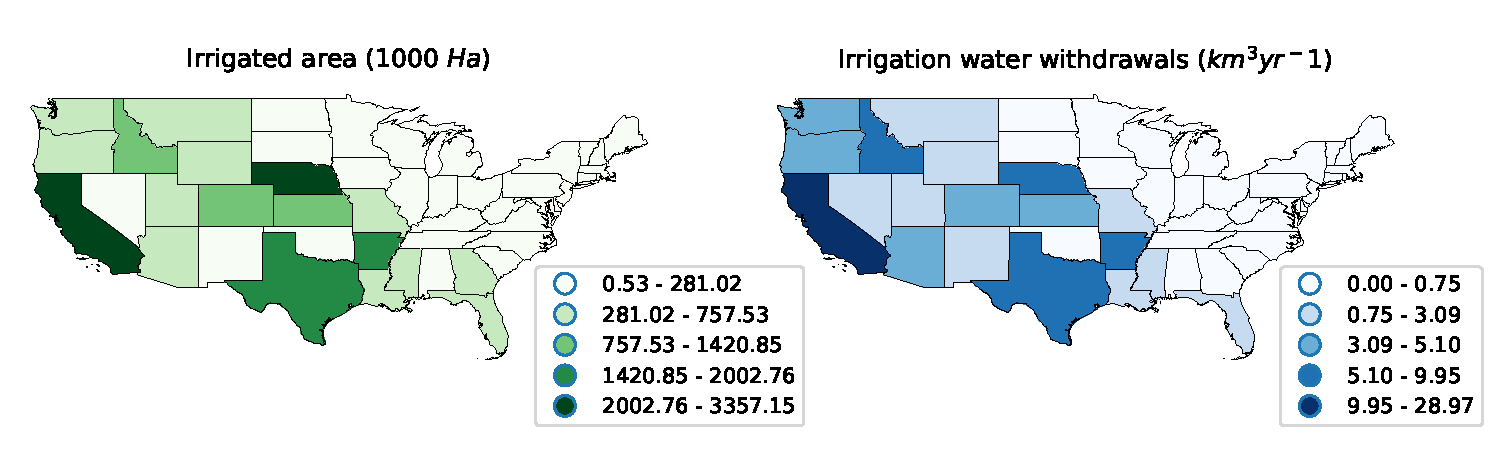
\includegraphics[width=\textwidth]{figures/background/fris2013_irrigation_volumes_and_area}
  \caption{\textbf{Per-state irrigated area and irrigation water withdrawals for 2013.} The data was drawn from the latest Farm and Ranch Irrigation Survey (FRIS) and only reflects irrigation operations in open fields (e.g. excluding crops grown and irrigated in greenhouses).}
  \label{fig:background-irrigation-area-volumes}
\end{figure}
%--------------------------------------------------------%
\begin{figure}[t]
  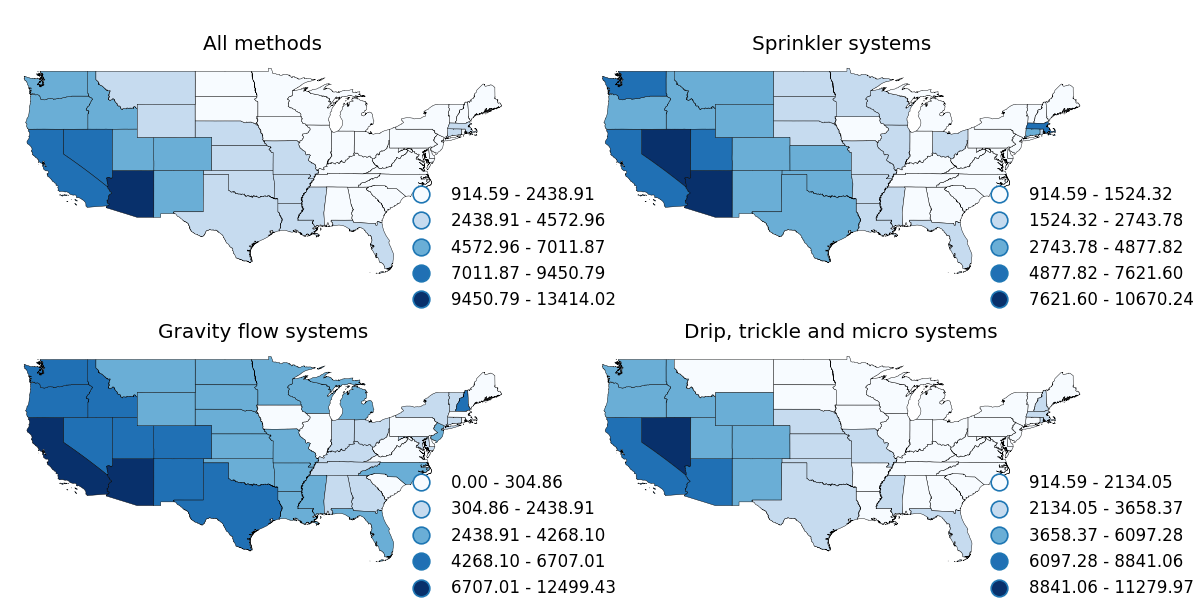
\includegraphics[width=\textwidth]{figures/background/fris2013_irrigation_volumes_per_method}
  \caption{\textbf{Per-state irrigation water application rates ($\unit{m^{3} ha^{-1}}$) by irrigation technique for 2013.} In accordance with figure~\ref{fig:background-irrigation-area-volumes}, the data was derived from the 2013 FRIS and only reflects irrigation operations in open fields.}
  \label{fig:background-irrigation-application-rates}
\end{figure}
%--------------------------------------------------------%
%	4) Methods
%--------------------------------------------------------%
\clearpage
\begin{figure}
   \centering
   % fig
   \begin{subfigure}[t]{0.49\textwidth}
       \centering
       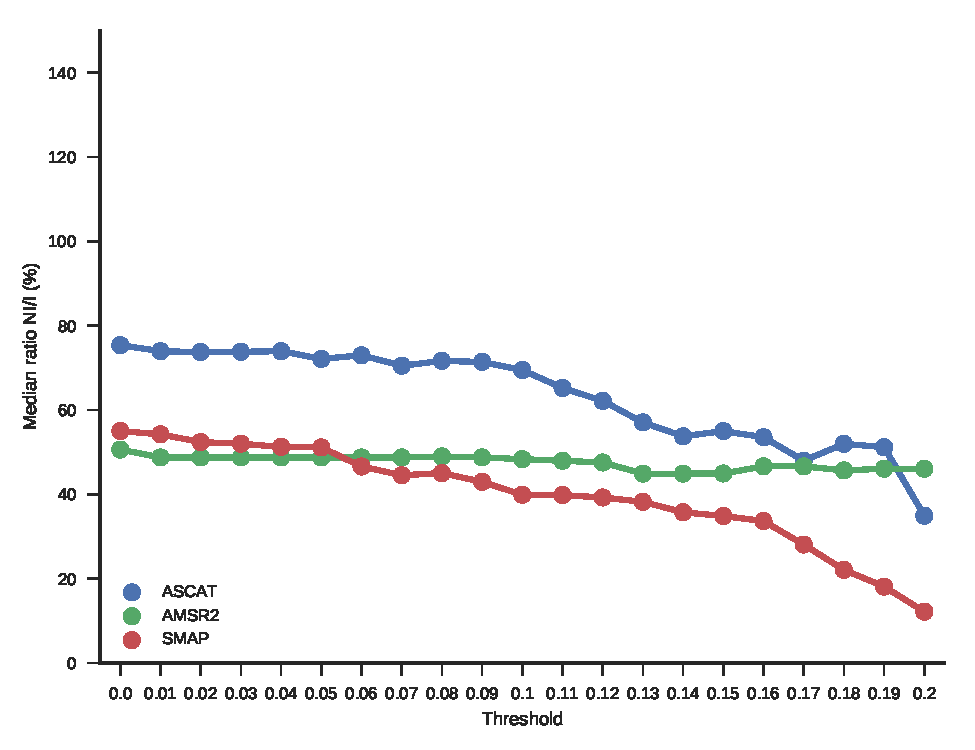
\includegraphics[width=\textwidth]{figures/methods/Southern_California_precmask_True}
       \caption{San Joaquin Valley, California}
       \label{fig:sensitivity-analysis-SJV}
   \end{subfigure}
   \hfill
   % fig
   \begin{subfigure}[t]{0.49\textwidth}
       \centering
       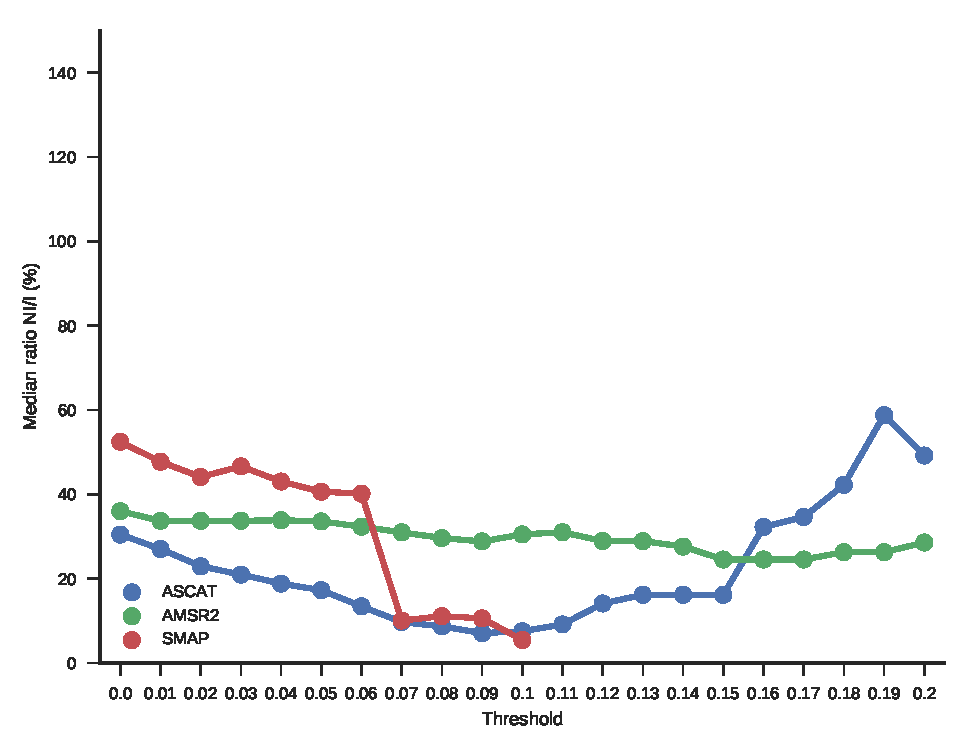
\includegraphics[width=\textwidth]{figures/methods/Idaho_precmask_True}
       \caption{Snake River Valley, Idaho}
       \label{fig:sensitivity-analysis-SRP}
   \end{subfigure}
   \hfill
   % fig
   \begin{subfigure}[t]{0.49\textwidth}
       \centering
       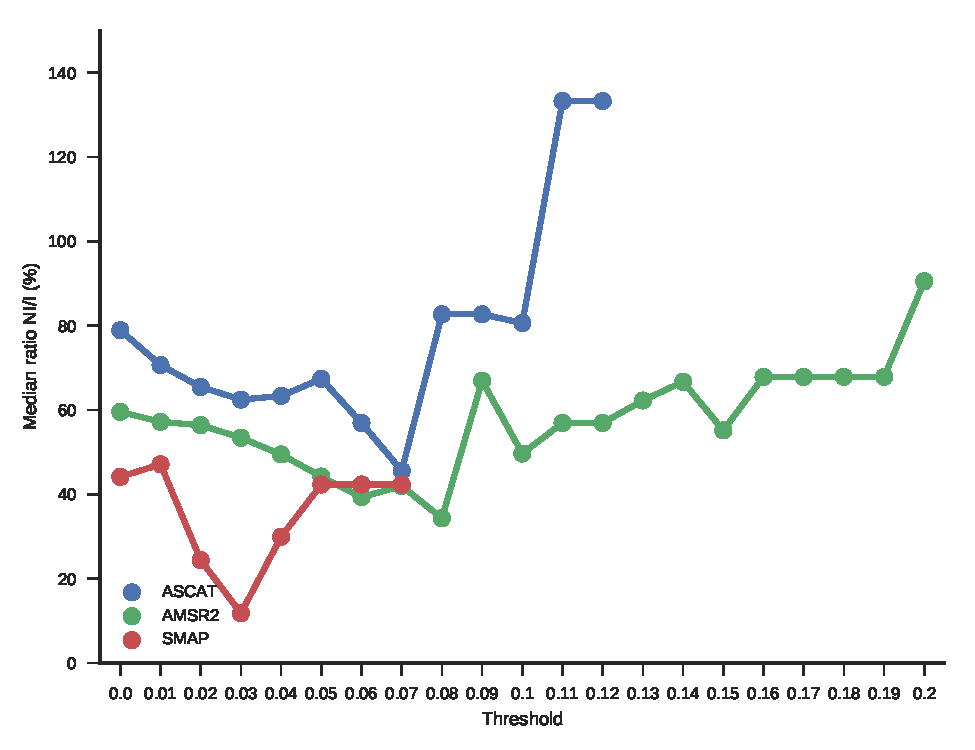
\includegraphics[width=\textwidth]{figures/methods/Nebraska_precmask_True}
       \caption{Nebraska plains}
       \label{fig:sensitivity-analysis-NPS}
   \end{subfigure}
   \hfill
   % fig
   \begin{subfigure}[t]{0.49\textwidth}
       \centering
       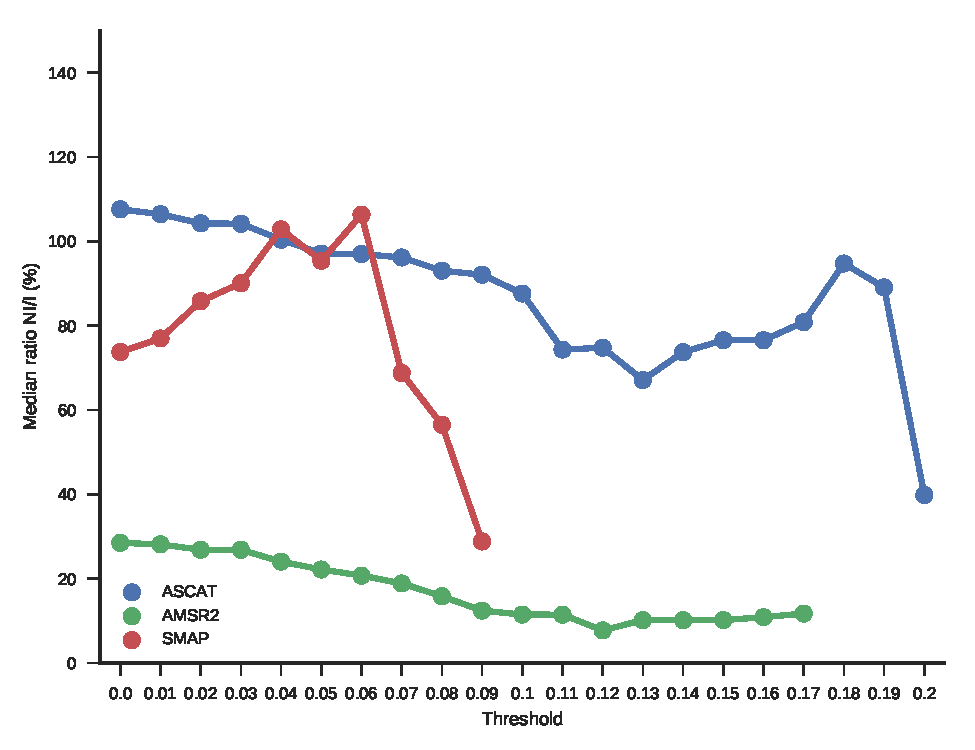
\includegraphics[width=\textwidth]{figures/methods/Mississippi_Delta_precmask_True}
       \caption{Mississippi Flood Plain}
       \label{fig:sensitivity-analysis-MFP}
   \end{subfigure} 
   \caption{\textbf{Sensitivity of the threshold defining an irrigation signal through the intensity of the relative increase in SM ($\frac{d \Theta_{sat}}{dt} \geq threshold$) to the skill of the method in differentiating between irrigated (PI) and non-irrigated (PNI) areas.} For each location, the ratio of irrigation water use (IWU) estimated at P-NI and P-I ($\frac{I_{PNI}}{I_{PI}} \times 100$) is plotted against thresholds of $0-20\%$.}
   \label{fig:sensitivity-analysis}
\end{figure}

\clearpage
\begin{figure}[t]
  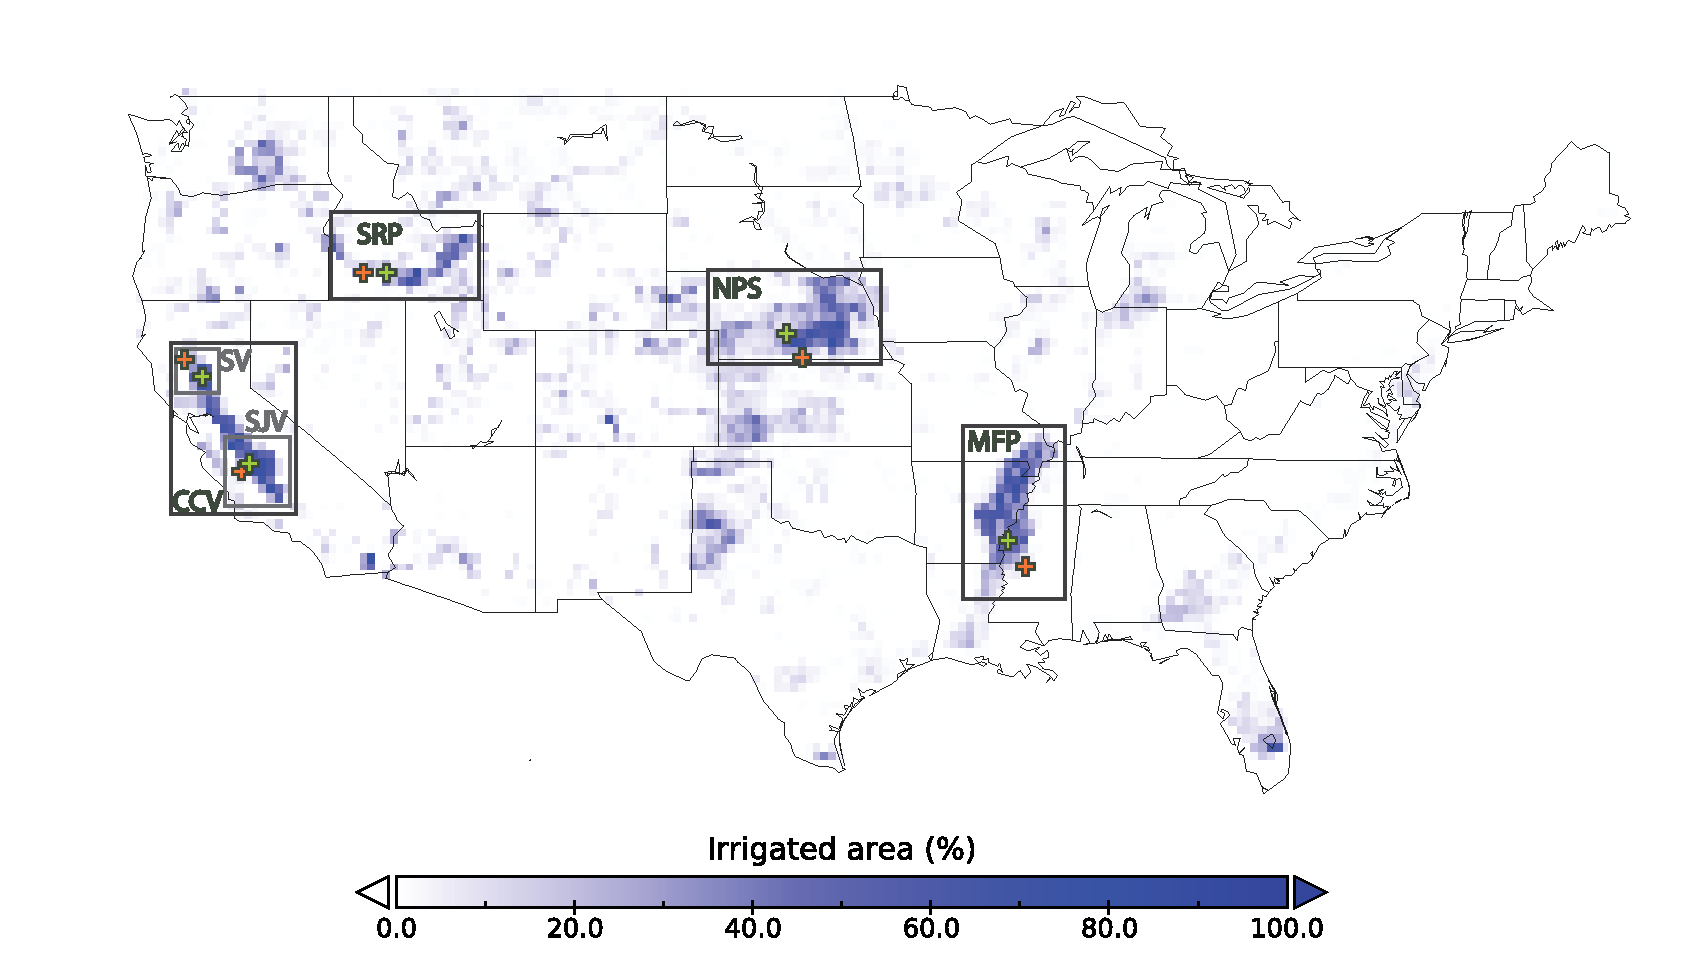
\includegraphics[width=\textwidth]{figures/mirad25km_study_areas_v3}
  \caption{\textbf{Study regions and locations of the pixels selected for a local time series analysis over the fractional irrigated area map derived from the spatially aggregated MIrAD-US data set \citep{Pervez_2010}.} From west to east the study regions are: the Sacramento Valley (SV) and San Joaquin Valley (SJV) within the California Central Valley (CCV), California; Snake River Plain (SRP), Idaho; Nebraska Plains (NPS), Nebraska; and the Mississippi Flood Plain (MFP), Mississippi. Green and orange crosses respectively indicate the locations of the irrigated (P-I) and non-irrigated (P-NI) pixels at which we further analyze satellite and model soil moisture time series in conjunction with IWU estimates.}
  \label{fig:study-areas-over-mirad}
\end{figure}

%--------------------------------------------------------%
%	5) Results
%--------------------------------------------------------%
\clearpage

% CORRELATION: spatial plots
\begin{figure}
   \centering
   % fig
   \begin{subfigure}[t]{0.55\textwidth}
       \centering
       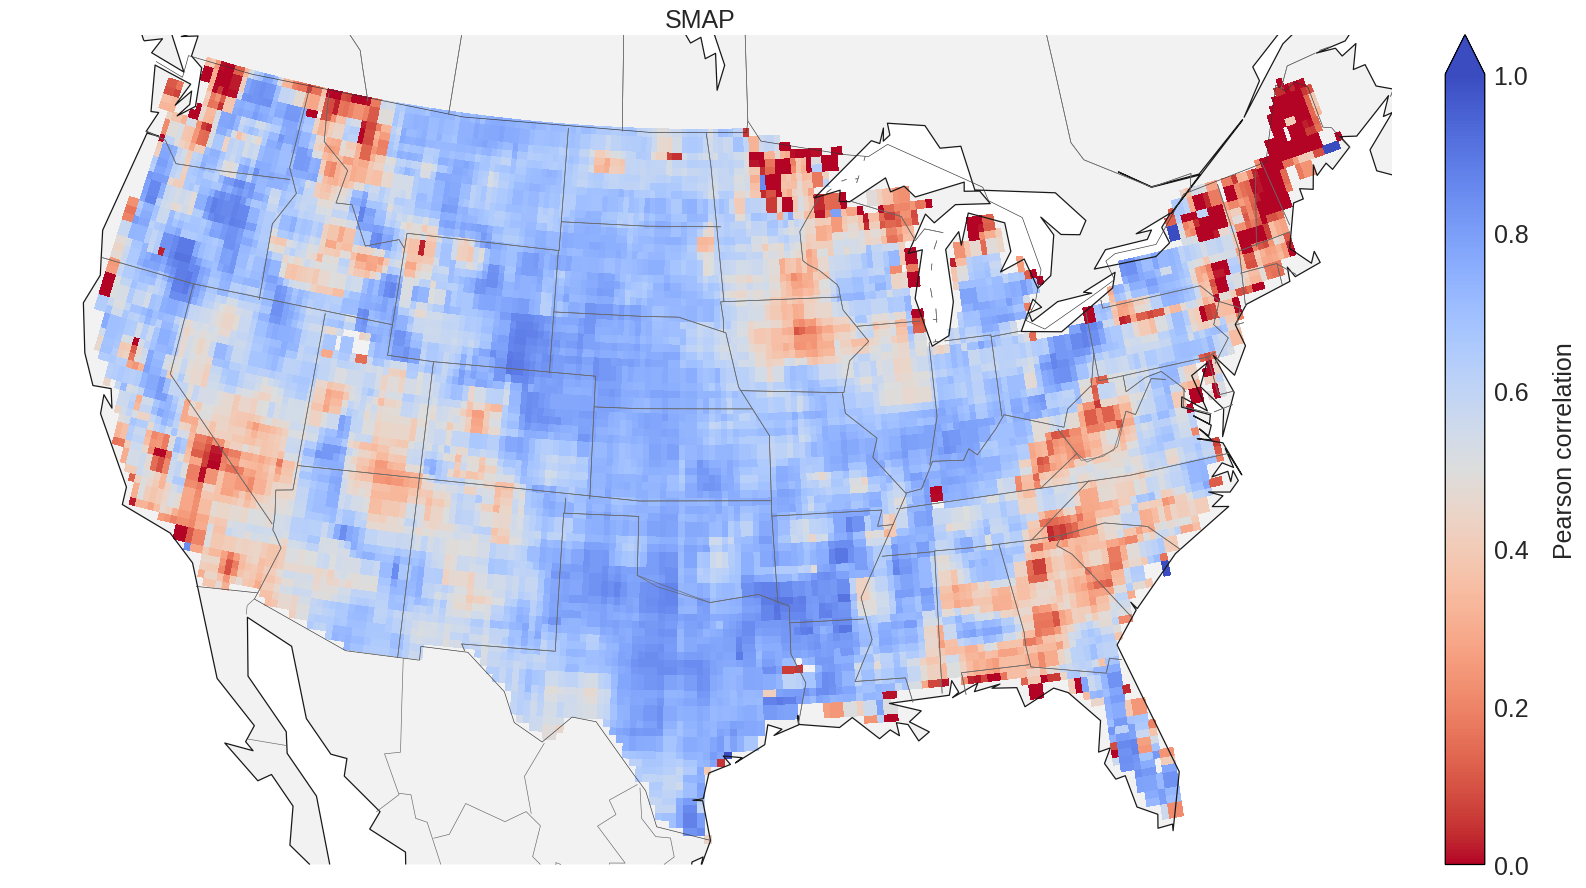
\includegraphics[width=\textwidth]{figures/results/corr_SMAP_MERRA2}
       \caption{}
       \label{fig:spatialplot-correlation-SMAP}
   \end{subfigure}
   \hfill
   % fig
   \begin{subfigure}[t]{0.55\textwidth}
       \centering
       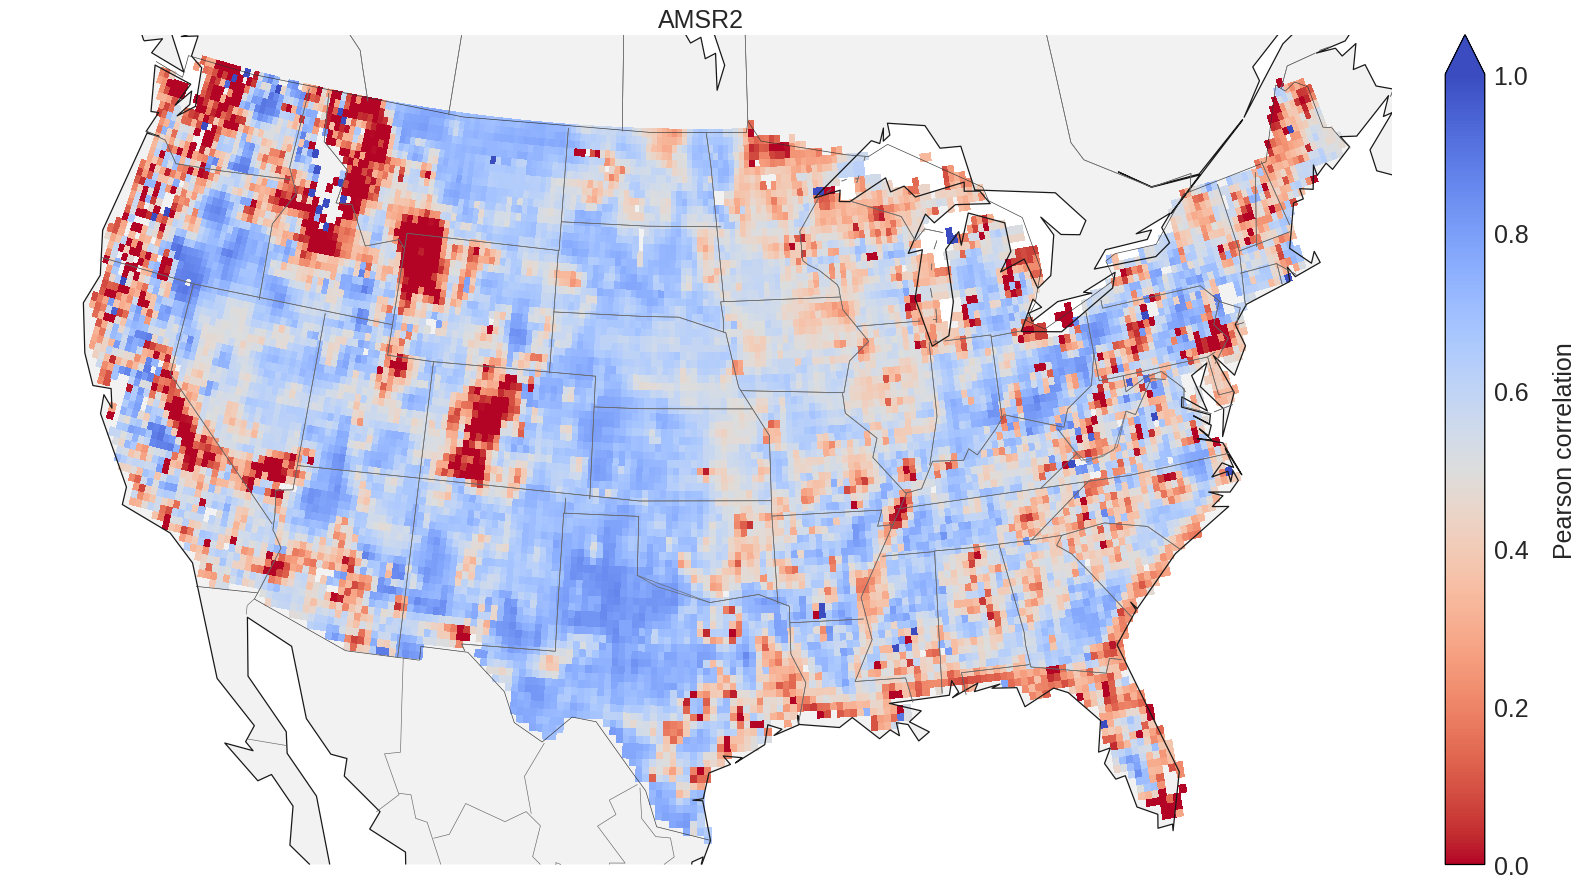
\includegraphics[width=\textwidth]{figures/results/corr_AMSR2_MERRA2}
       \caption{}
       \label{fig:spatialplot-correlation-AMSR2}
   \end{subfigure}
   \hfill
   % fig
   \begin{subfigure}[t]{0.55\textwidth}
       \centering
       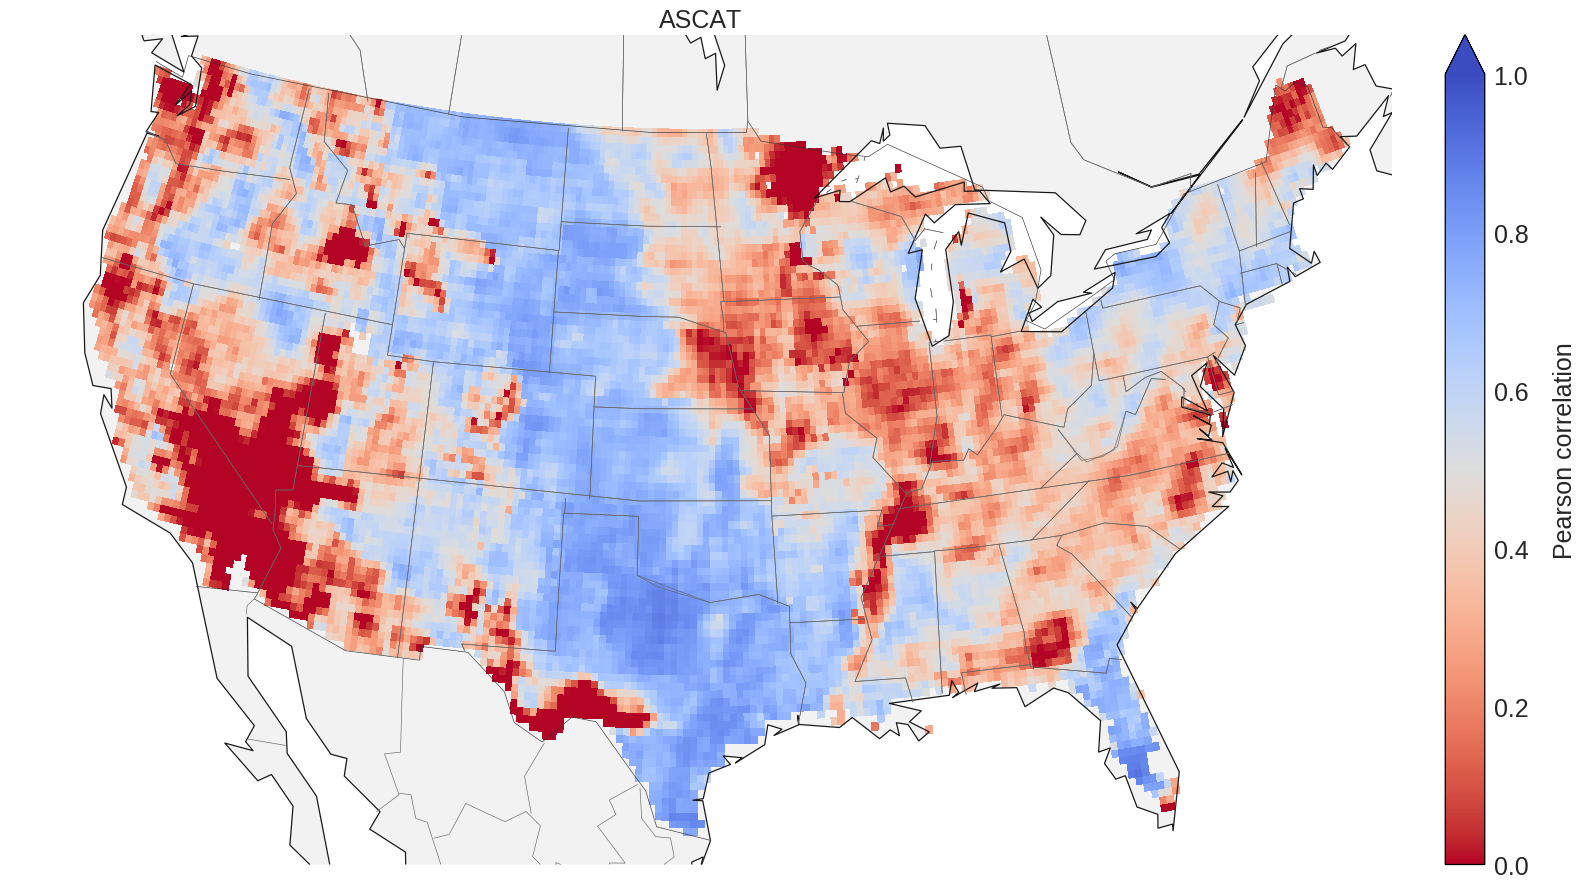
\includegraphics[width=\textwidth]{figures/results/corr_ASCAT_MERRA2}
       \caption{}
       \label{fig:spatialplot-correlation-ASCAT}
   \end{subfigure}
   \caption{\textbf{Mean rowing season correlations $\overline{R}_{GWS}$ between the daily time series of each satellite soil moisture product (SMAP, AMSR2 and ASCAT) with MERRA-2 soil moisture.} The Pearson's correlation coefficient was calculated for each growing season (April-September) from 2013-2016 for SMAP (\ref{fig:spatialplot-correlation-SMAP}), AMSR2 (\ref{fig:spatialplot-correlation-AMSR2}) and ASCAT (\ref{fig:spatialplot-correlation-ASCAT}) soil moisture products (note that SMAP data only was available from 2015/04 onwards).}
   \label{fig:spatialplot-correlation}
\end{figure}

% CORRELATION: scatter corr - irrigation fraction
\begin{figure}[t]
  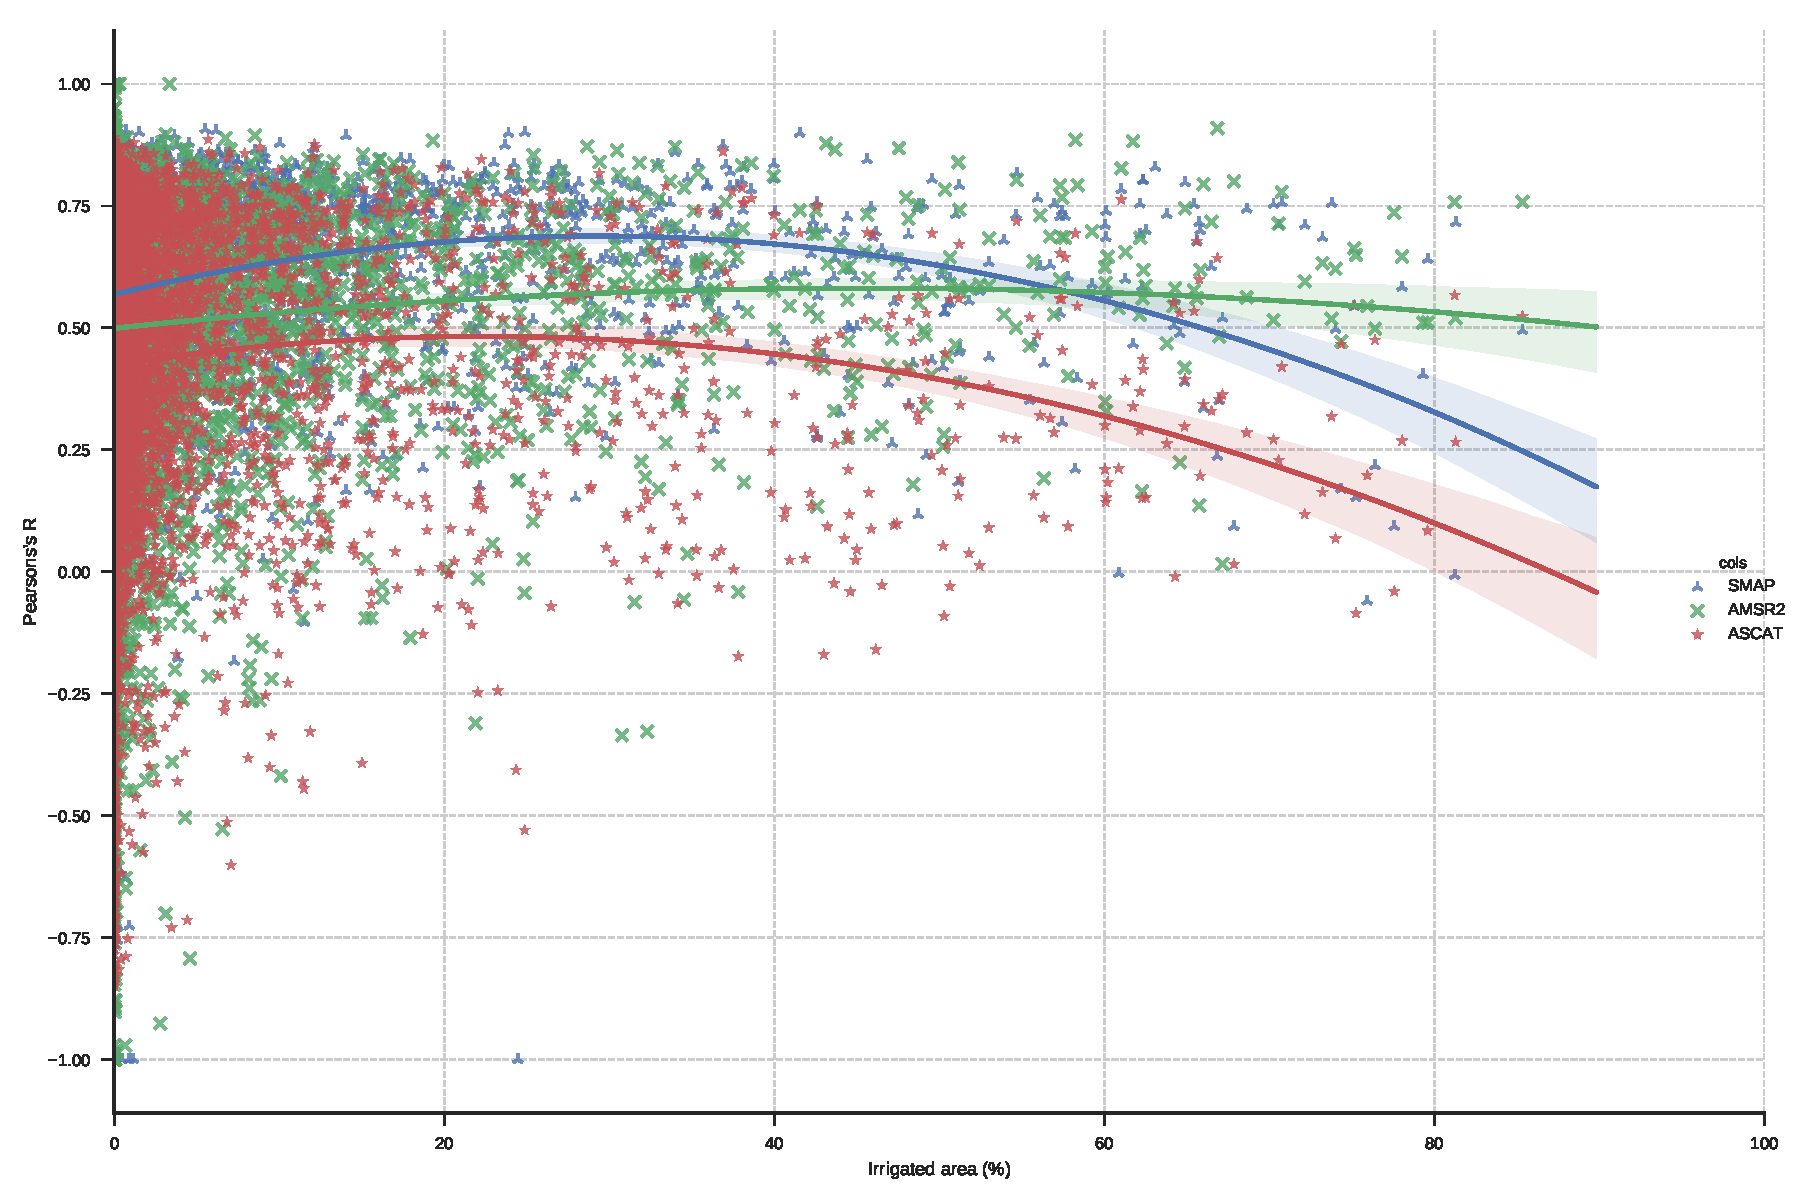
\includegraphics[width=\textwidth]{figures/correlation/scatter_corr_irrigation_fraction_v2_2nd_order_fit}
  \caption{\textbf{Relationship of $\overline{r}_{GWS}$ between each satellite-model pair with fractional irrigated area derived from the spatially aggregated MIrAD-US.} For each combination, a second order polynomial regression was fitted and plotted with the respective 95\% confidence intervals (shading).}
  \label{fig:scatterplot-corr-irrigfrac}
\end{figure}

%--------------------------------------------------------%
\clearpage
% MULTIANNUAL CLIMS
\begin{figure}
   \centering
   % fig
   \begin{subfigure}[t]{0.52\textwidth}
       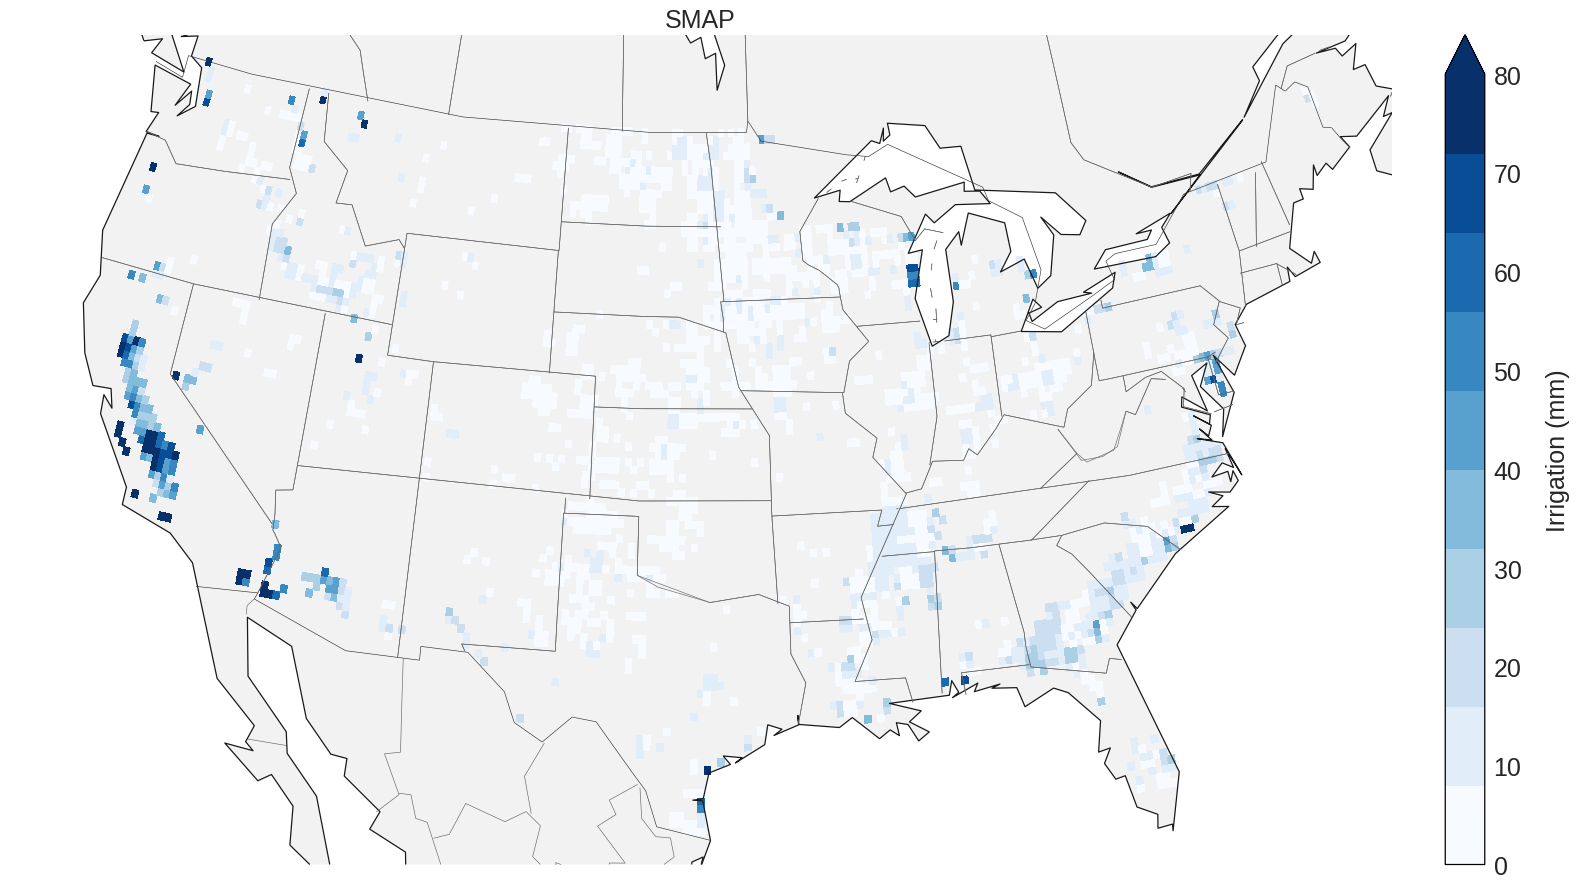
\includegraphics[width=\textwidth]{figures/results/SMAP_multiannual_clim_thresh_0_05_irrig_signals}
       \caption{}
       \label{fig:spatialplot-multiannualirrigation-SMAP}
   \end{subfigure}
   % fig
   \begin{subfigure}[t]{0.52\textwidth}
       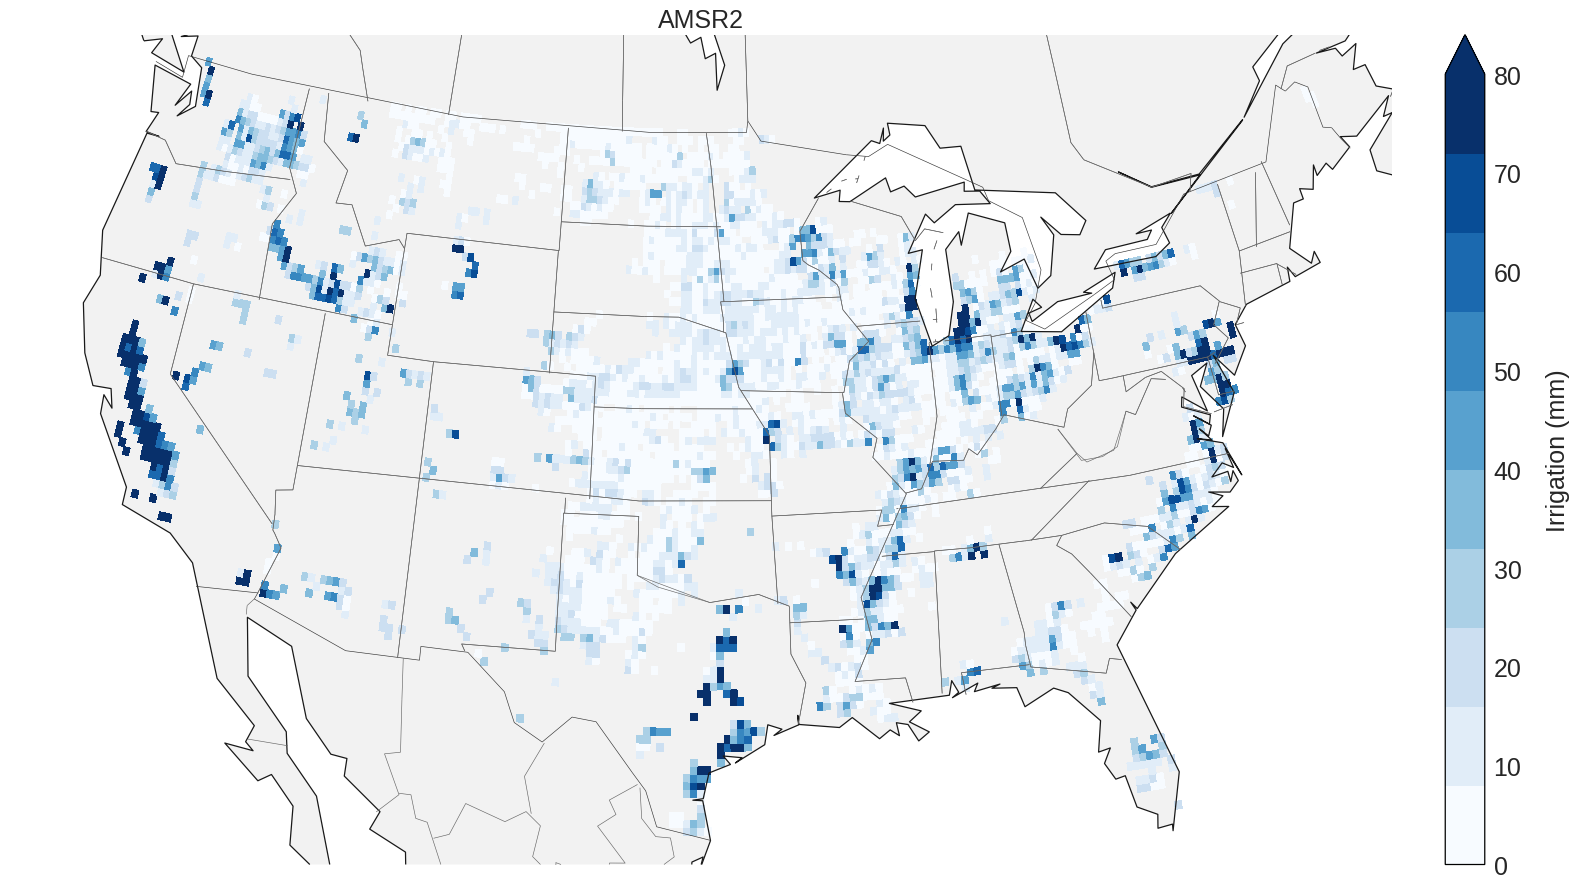
\includegraphics[width=\textwidth]{figures/results/AMSR2_multiannual_clim_thresh_0_05_irrig_signals}
   	   \caption{}
       \label{fig:spatialplot-multiannualirrigation-AMSR2}
   \end{subfigure}
   % fig
   \begin{subfigure}[t]{0.52\textwidth}
       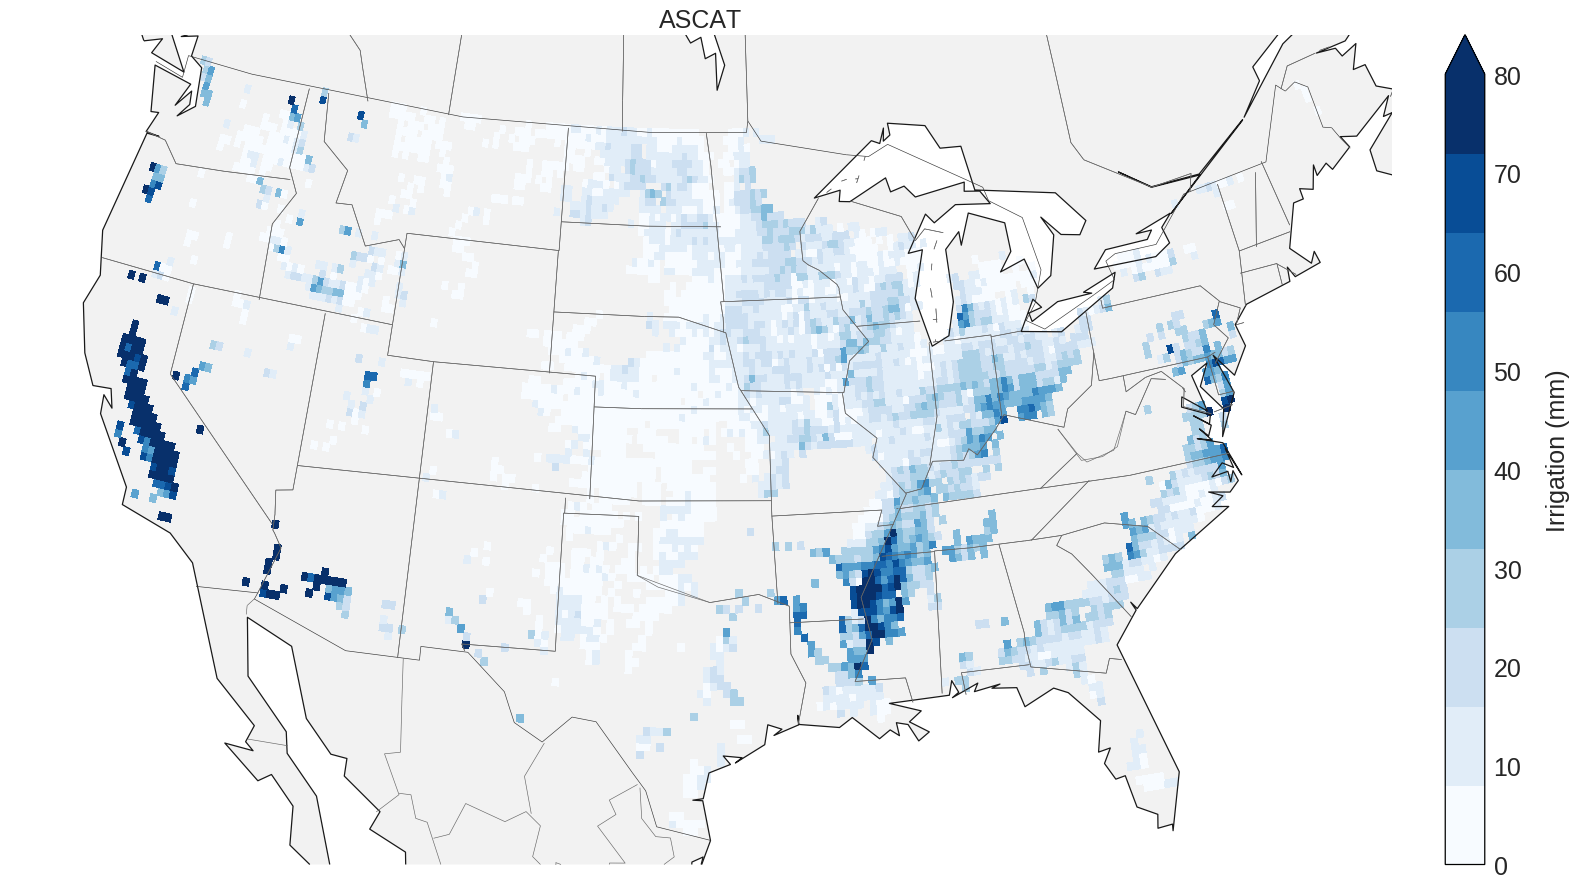
\includegraphics[width=\textwidth]{figures/results/ASCAT_multiannual_clim_thresh_0_05_irrig_signals}
   	   \caption{}
       \label{fig:spatialplot-multiannualirrigation-ASCAT}
   \end{subfigure}
   \caption{\textbf{Mean annual irrigation water use $\overline{IWU}_{A}$ derived from SMAP (\ref{fig:spatialplot-multiannualirrigation-SMAP}), AMSR2 (\ref{fig:spatialplot-multiannualirrigation-AMSR2}) and ASCAT SM (\ref{fig:spatialplot-multiannualirrigation-ASCAT}) in combination with modeled SM from MERRA-2.} All pixels with a cropland fraction of $< 5\%$ (as inferred from the CCI land cover product) were excluded from the analysis (grey areas). Note that for SMAP the climatologies represent the growing season mean of 2015 and 2016, while for AMSR2 and ASCAT the estimates are derived from 4 years of data covering the period of 2013-2016. The upper limit of the colorbar is fixed at the 99th percentile of the SMAP based estimates.}
   \label{fig:spatialplot-multiannualirrigation}
\end{figure}
%--------------------------------------------------------%
\clearpage
% TIMESERIES
% sub figs
\begin{figure}
   \centering
   % fig
   \begin{subfigure}[t]{0.7\textwidth}
       \centering
       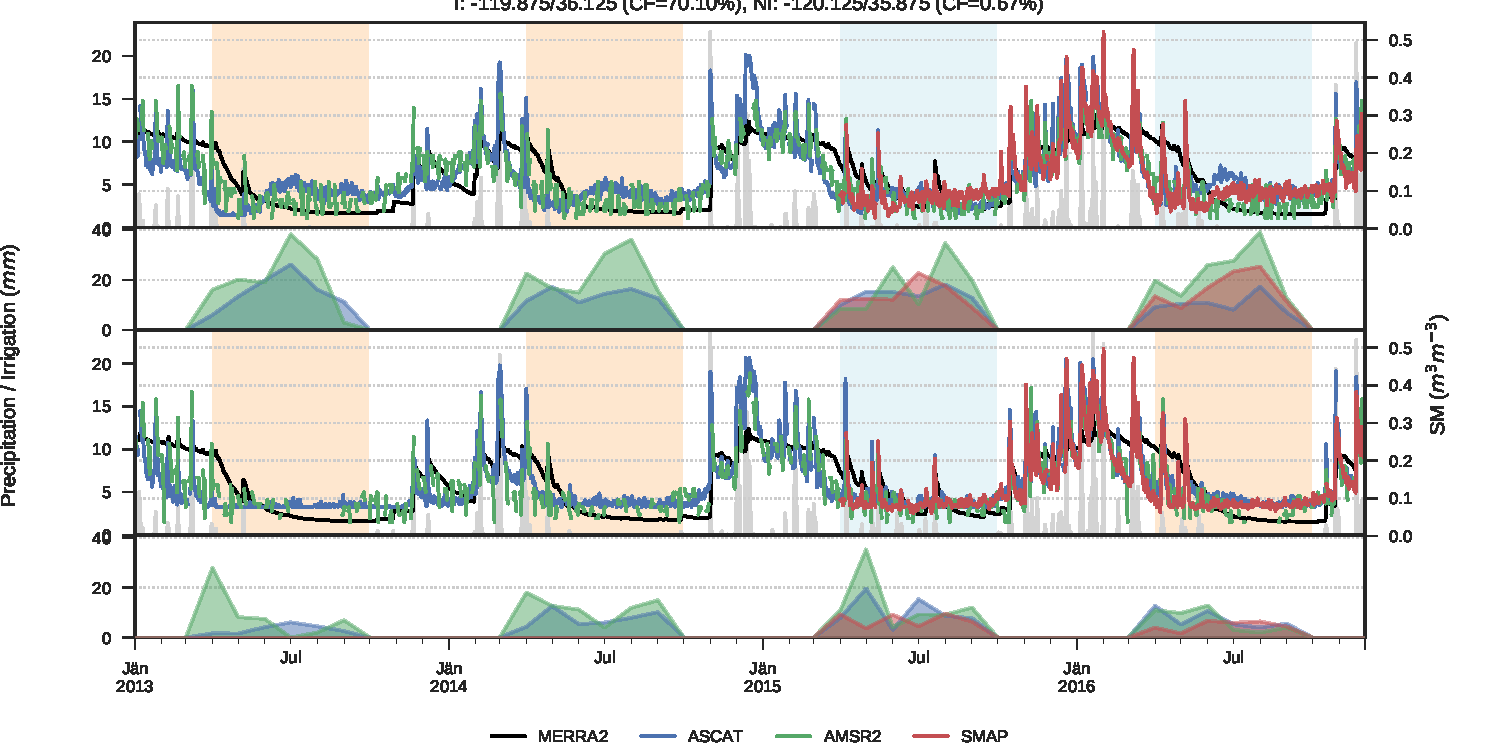
\includegraphics[width=\textwidth]{figures/results/California_Central_Valley}
       \caption{San Joaquin Valley (SJV), California}
       \label{fig:timeseries-SJV}
   \end{subfigure}
   \hfill
   % fig
   \begin{subfigure}[t]{0.7\textwidth}
       \centering
       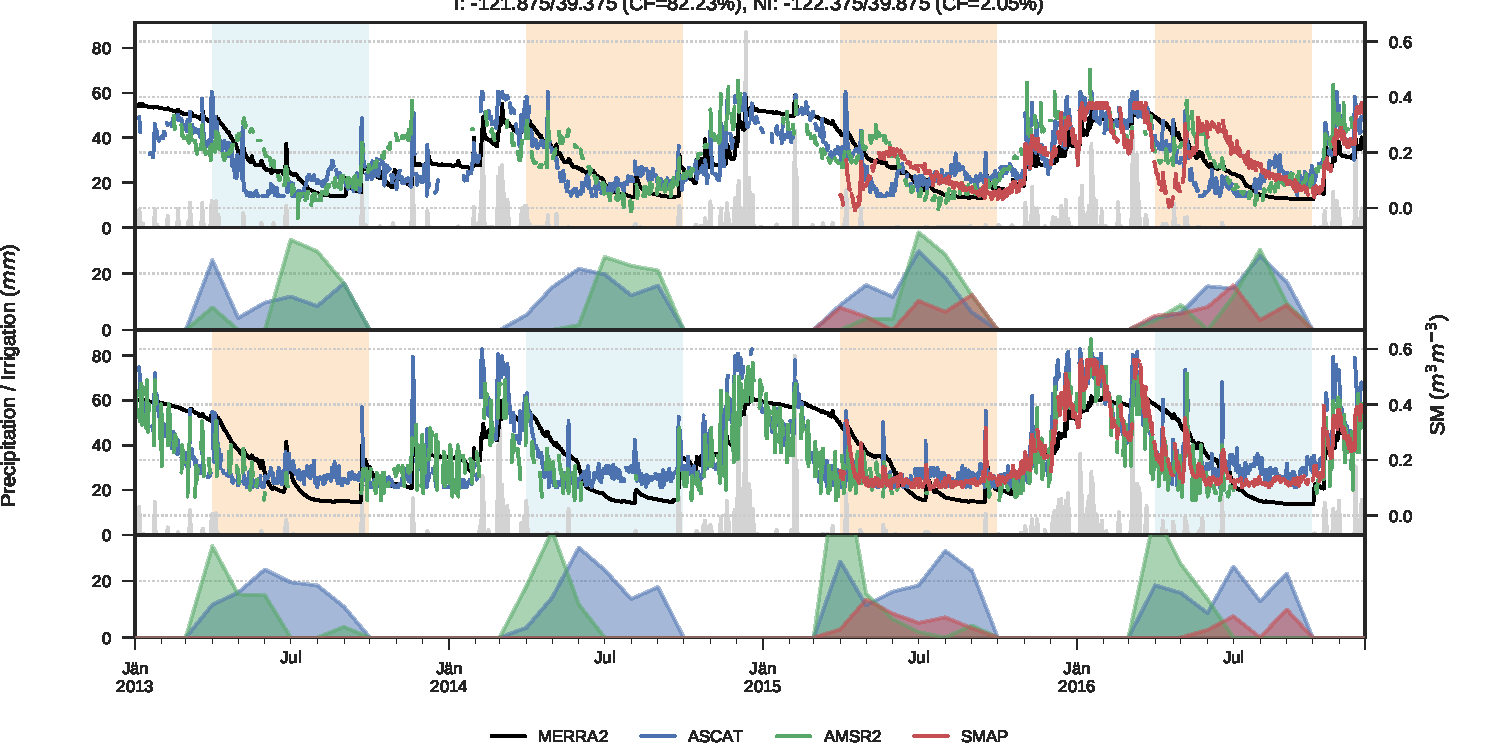
\includegraphics[width=\textwidth]{figures/results/California_Sacramento_Valley}
       \caption{Sacramento Valley (SV), California}
       \label{fig:timeseries-SV}
   \end{subfigure}
   \hfill
   % fig
   \begin{subfigure}[t]{0.7\textwidth}
       \centering
       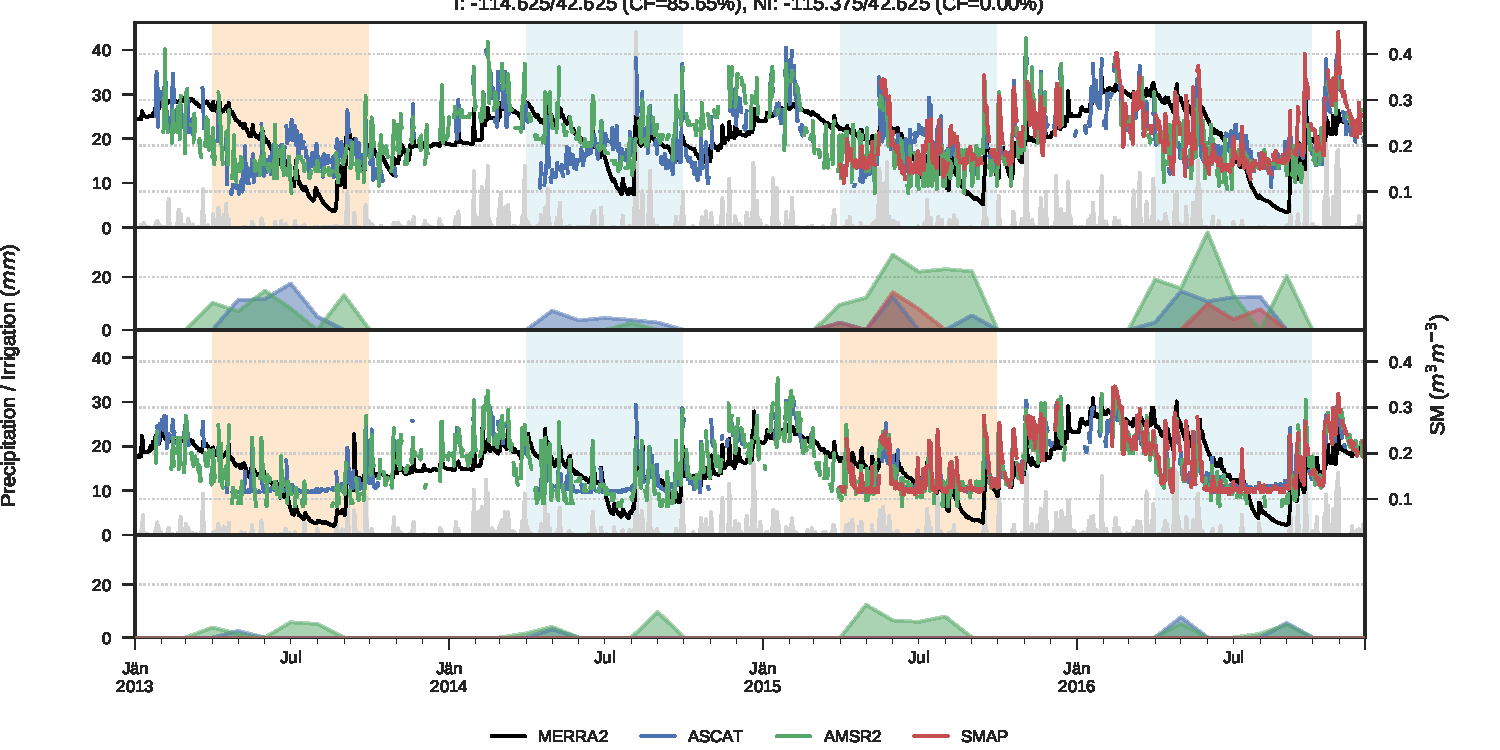
\includegraphics[width=\textwidth]{figures/results/Idaho}
       \caption{Snake River Plain (SRP), Idaho}
       \label{fig:timeseries-SRP}
   \end{subfigure}
\end{figure}
\begin{figure}\ContinuedFloat
   \centering
   % fig
   \begin{subfigure}[t]{0.7\textwidth}
       \centering
       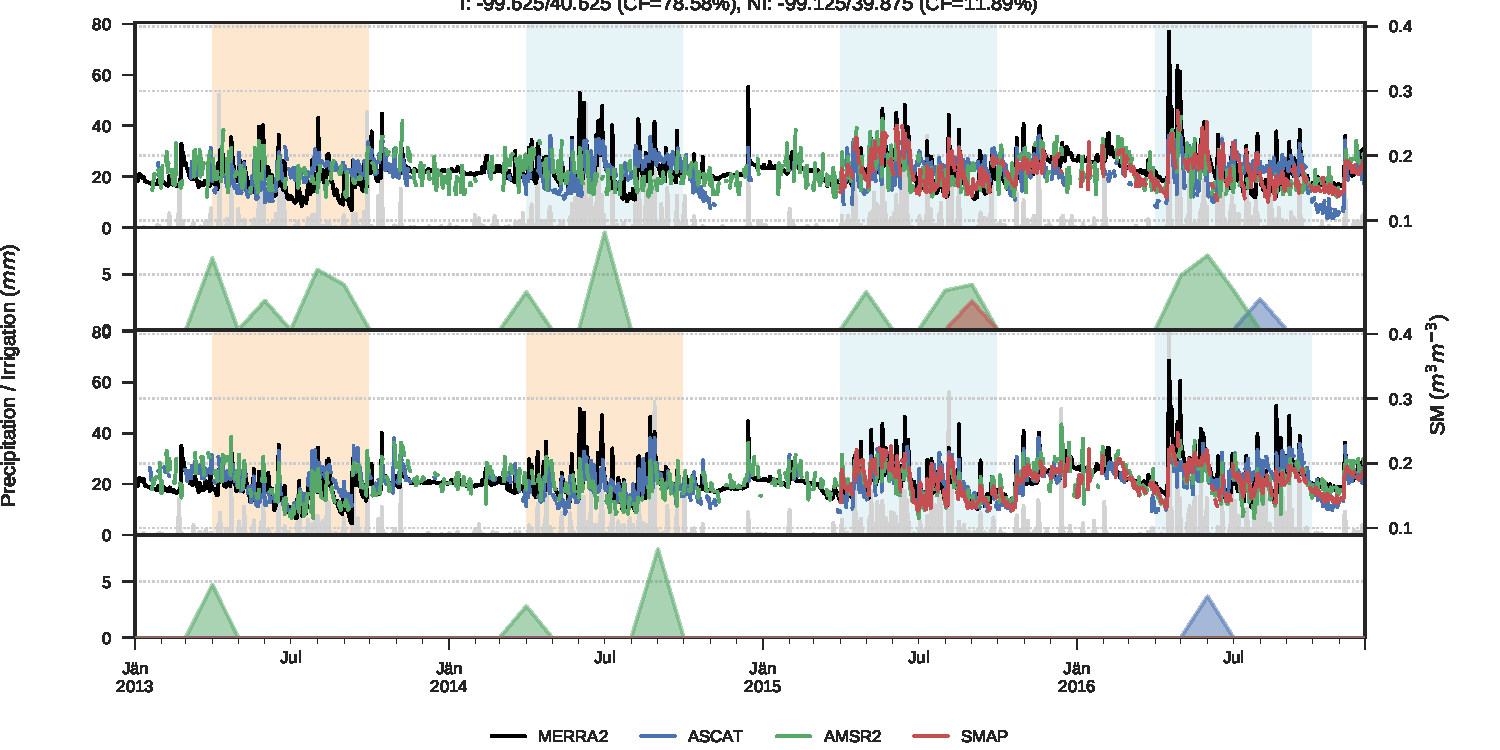
\includegraphics[width=\textwidth]{figures/results/Nebraska_plains}
       \caption{Plains of Nebraska (NPS), Nebraska}
       \label{fig:timeseries-NPS}
   \end{subfigure}
   \hfill
   \begin{subfigure}[t]{0.7\textwidth}
       \centering
       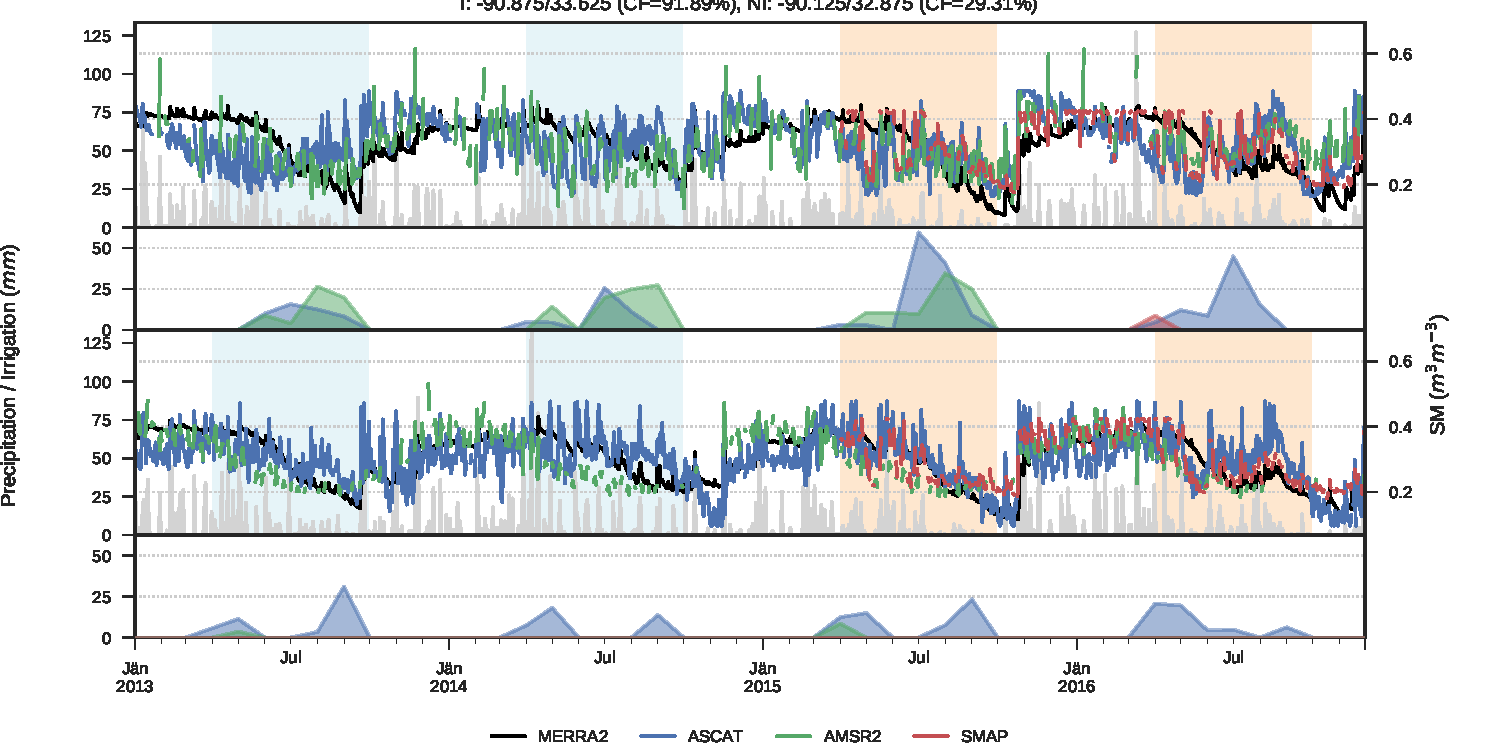
\includegraphics[width=\textwidth]{figures/results/Mississippi_Flood_Plain}
       \caption{Lower Mississippi Floodplain (MFP), Mississippi}
       \label{fig:timeseries-MFP}
   \end{subfigure}
   \hfill
   \caption{\textbf{Comparison of satellite and model soil moisture time series at irrigated (top two sub-panels) and non-irrigated pixels (bottom two sub-panels) in four regions (figures~\ref{fig:timeseries-SJV} - \ref{fig:timeseries-MFP}).} Daily CPC precipitation is plotted in grey, while blue and orange shadings in the top sub-panels indicate positive and negative rainfall anomalies with respect to the growing season. The bottom sub-panels show the monthly irrigation water use estimates ($IWU_{M}$) obtained for each satellite-model pair (non-growing season periods have been masked).}
   \label{fig:timeseries}
\end{figure}

% %--------------------------------------------------------%
% \clearpage
% % MONTHLY CLIMATOLOGIES
% %--------------------------------------------------------%
% \begin{figure}
%    \centering
%    % APRIL
%    \begin{subfigure}[b]{0.3\textwidth}
%        \centering
%        \caption{SMAP}
%        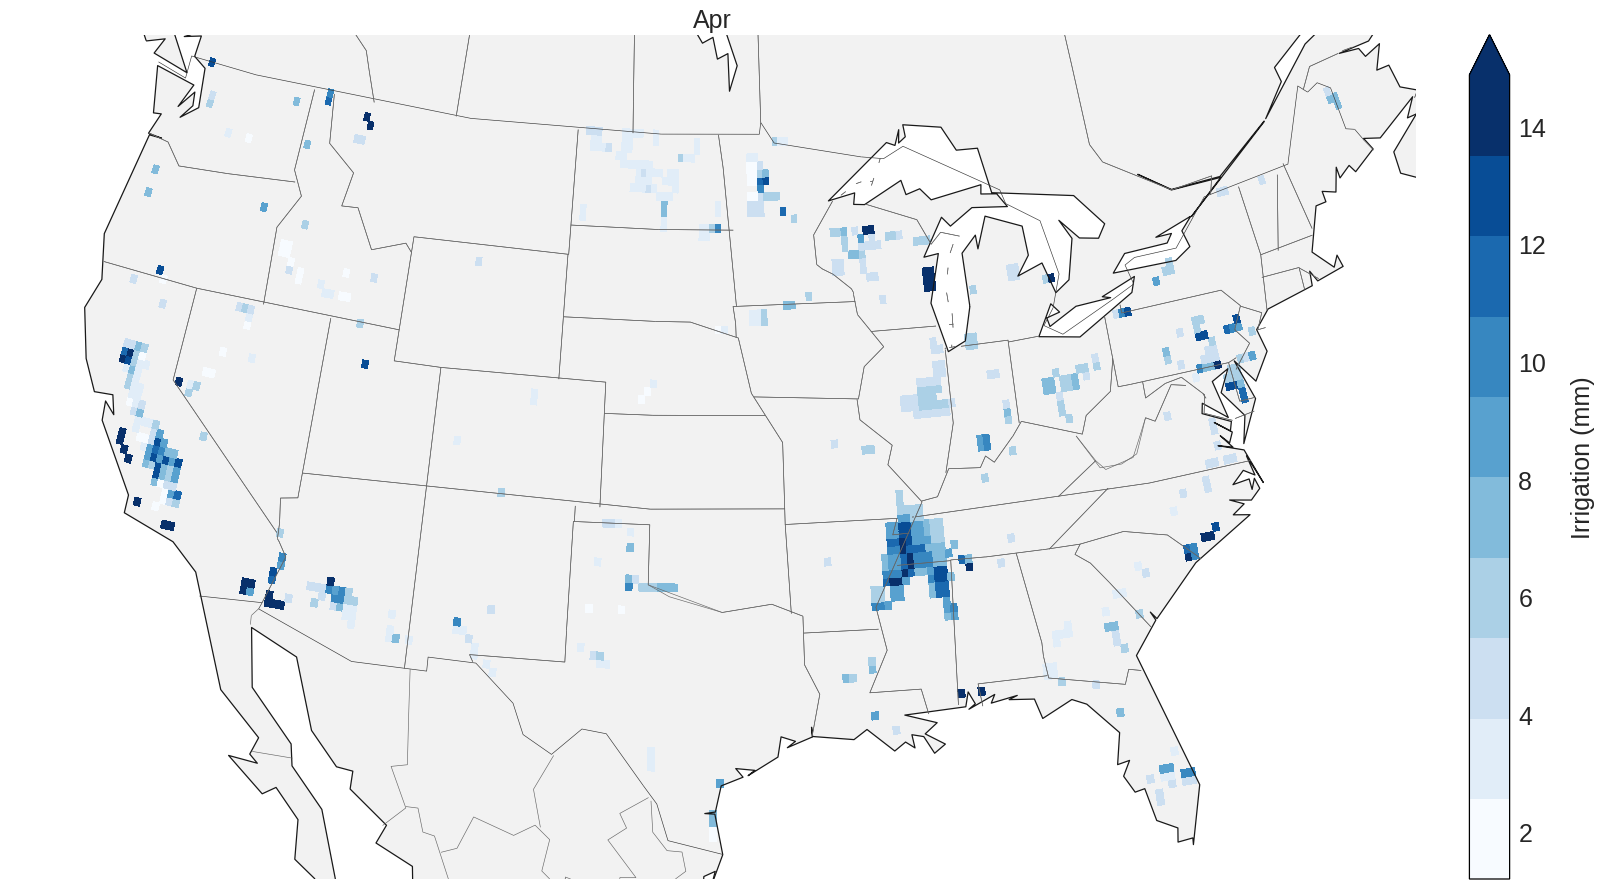
\includegraphics[width=\textwidth]{figures/monthly_clims/SMAP_monthly_clim_thresh_0_05_Apr}
%    \end{subfigure}
%    \hfill
%    \begin{subfigure}[b]{0.3\textwidth}
%        \centering
%        \caption{AMSR2}
%        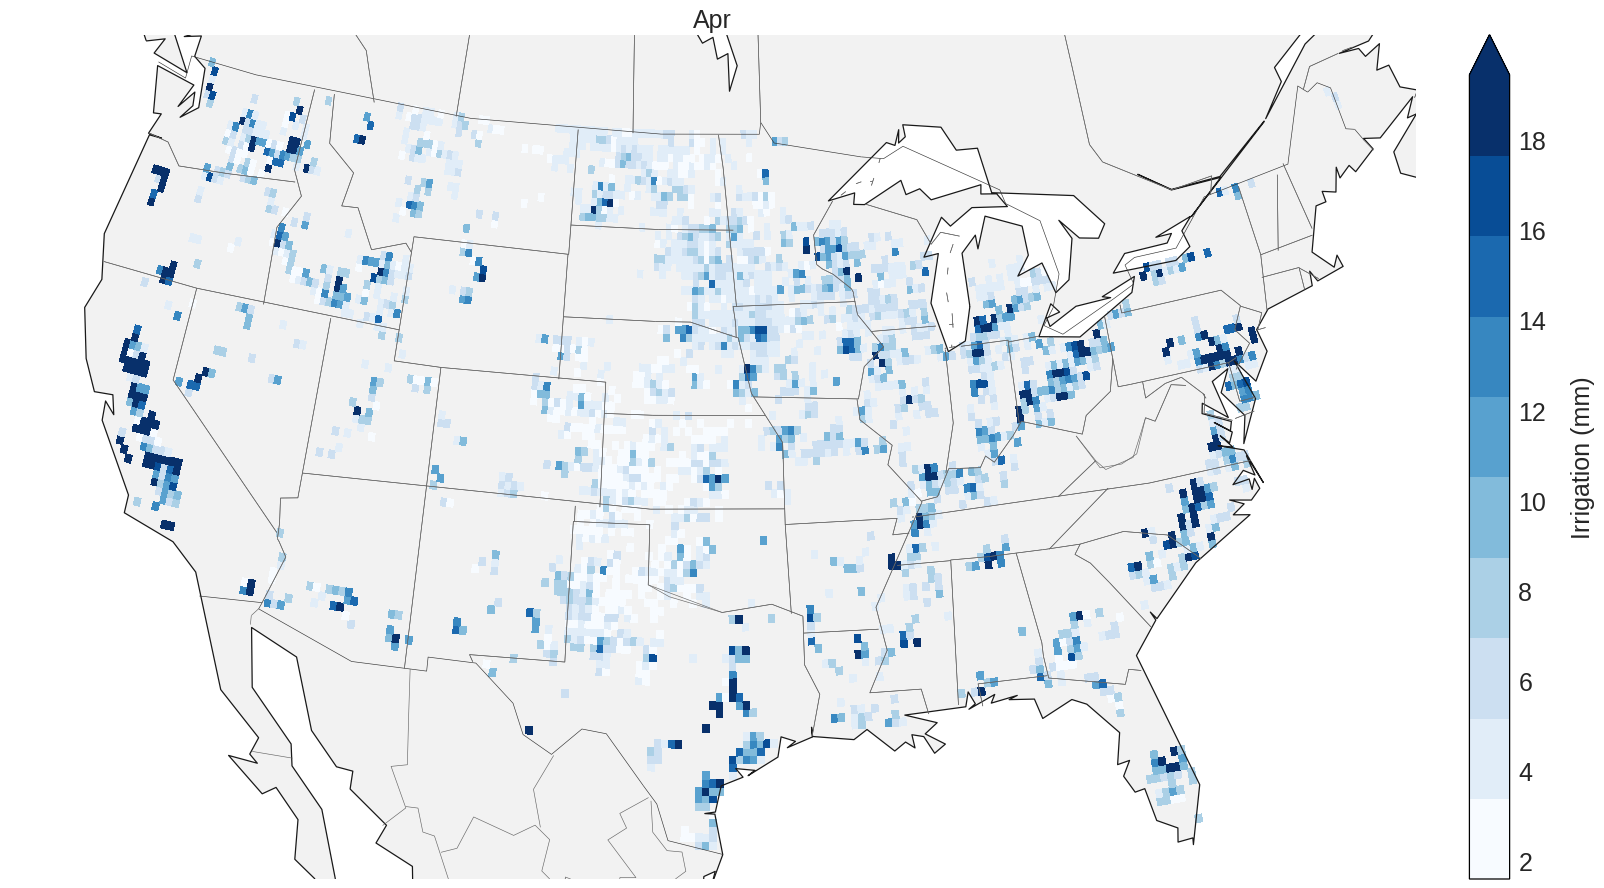
\includegraphics[width=\textwidth]{figures/monthly_clims/AMSR2_monthly_clim_thresh_0_05_Apr}
%    \end{subfigure}
%    \hfill
%    \begin{subfigure}[b]{0.3\textwidth}
%        \centering
%        \caption{ASCAT}
%        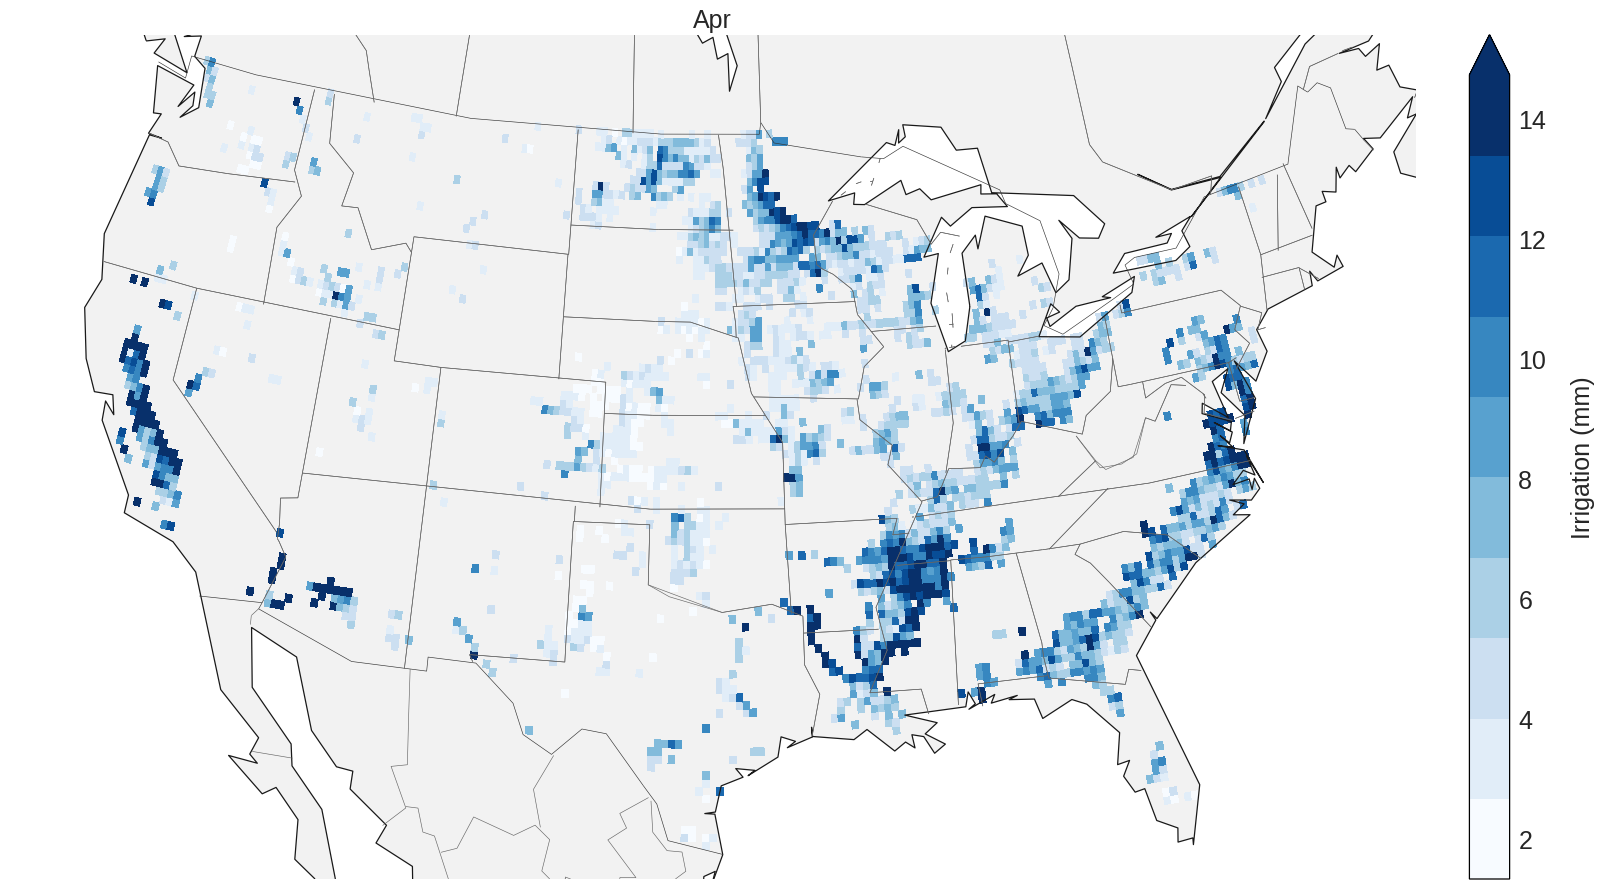
\includegraphics[width=\textwidth]{figures/monthly_clims/ASCAT_monthly_clim_thresh_0_05_Apr}
%    \end{subfigure}
%    \hfill   
%    % MAY
%    \begin{subfigure}[b]{0.3\textwidth}
%        \centering
%        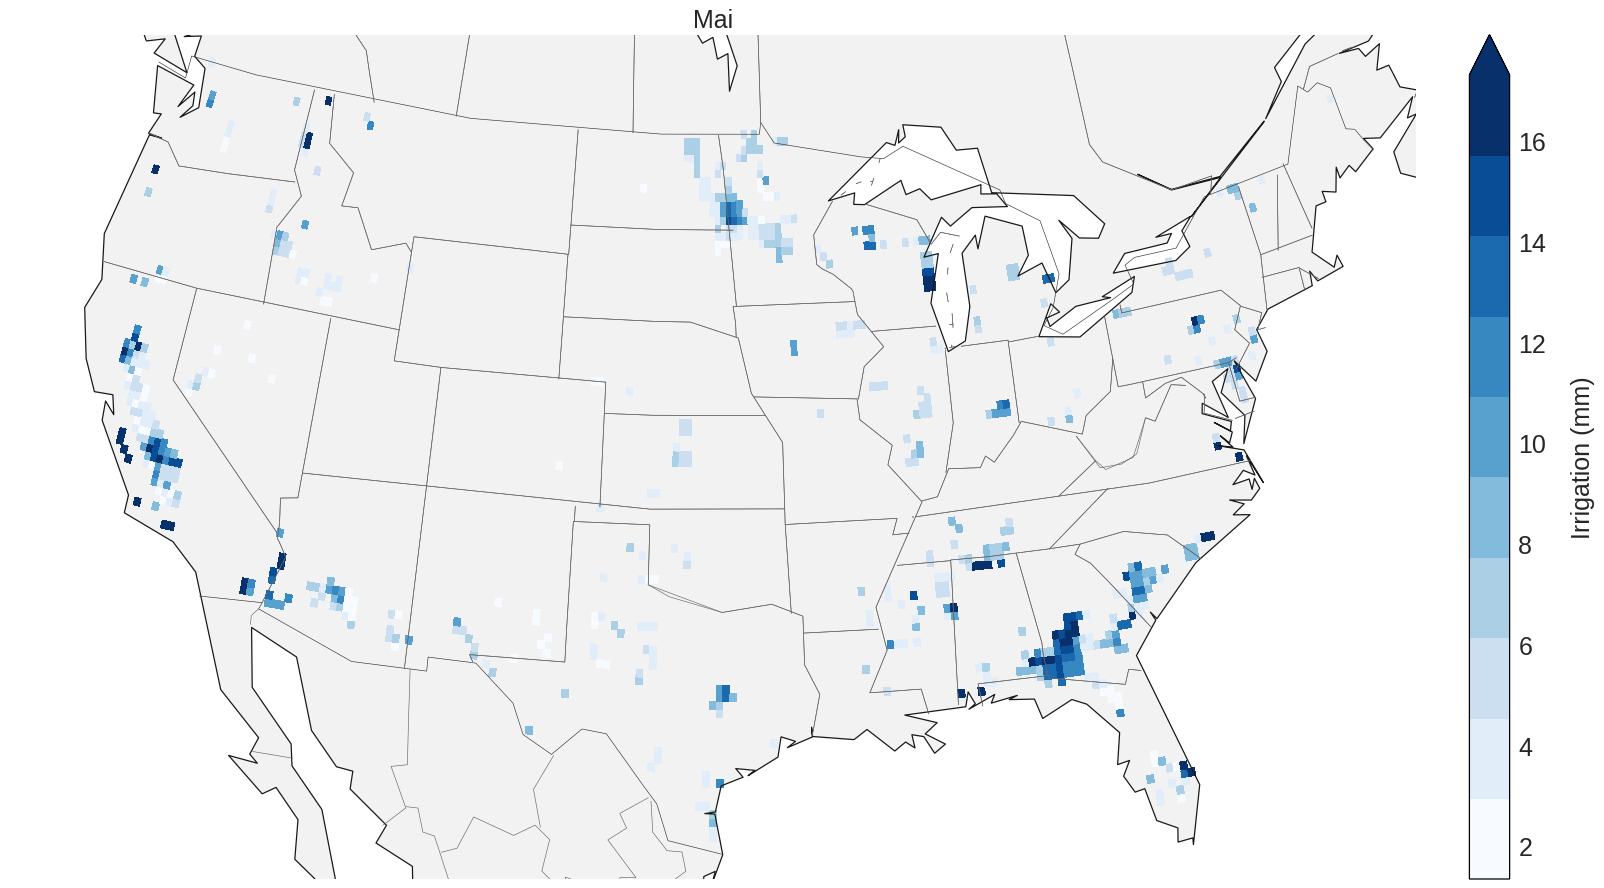
\includegraphics[width=\textwidth]{figures/monthly_clims/SMAP_monthly_clim_thresh_0_05_Mai}
%    \end{subfigure}
%    \hfill
%    \begin{subfigure}[b]{0.3\textwidth}
%        \centering
%        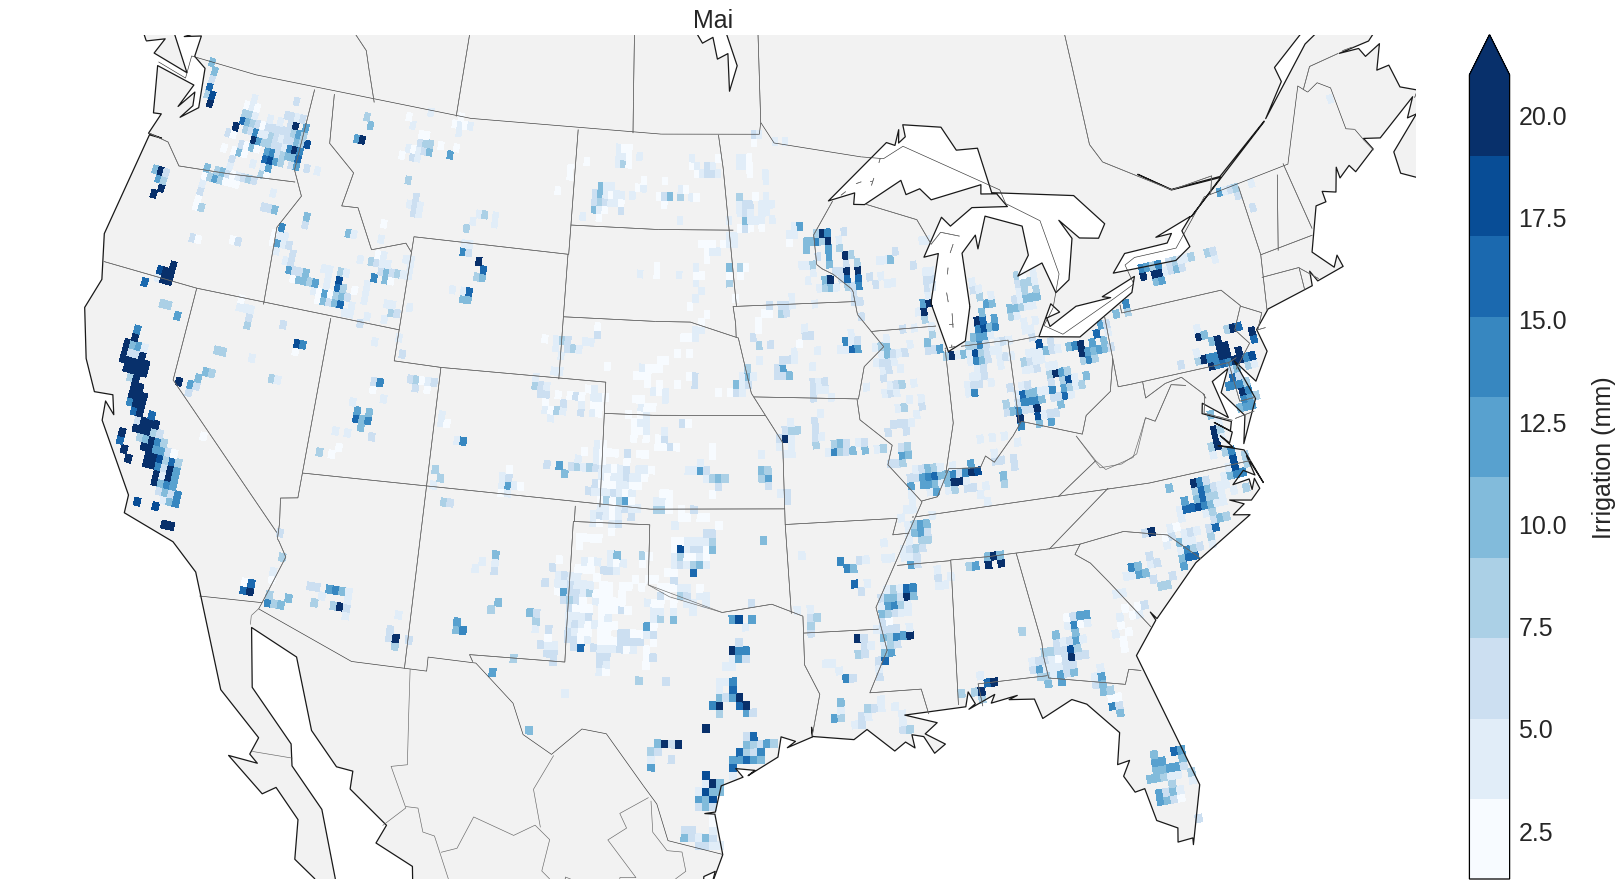
\includegraphics[width=\textwidth]{figures/monthly_clims/AMSR2_monthly_clim_thresh_0_05_Mai}
%    \end{subfigure}
%    \hfill
%    \begin{subfigure}[b]{0.3\textwidth}
%        \centering
%        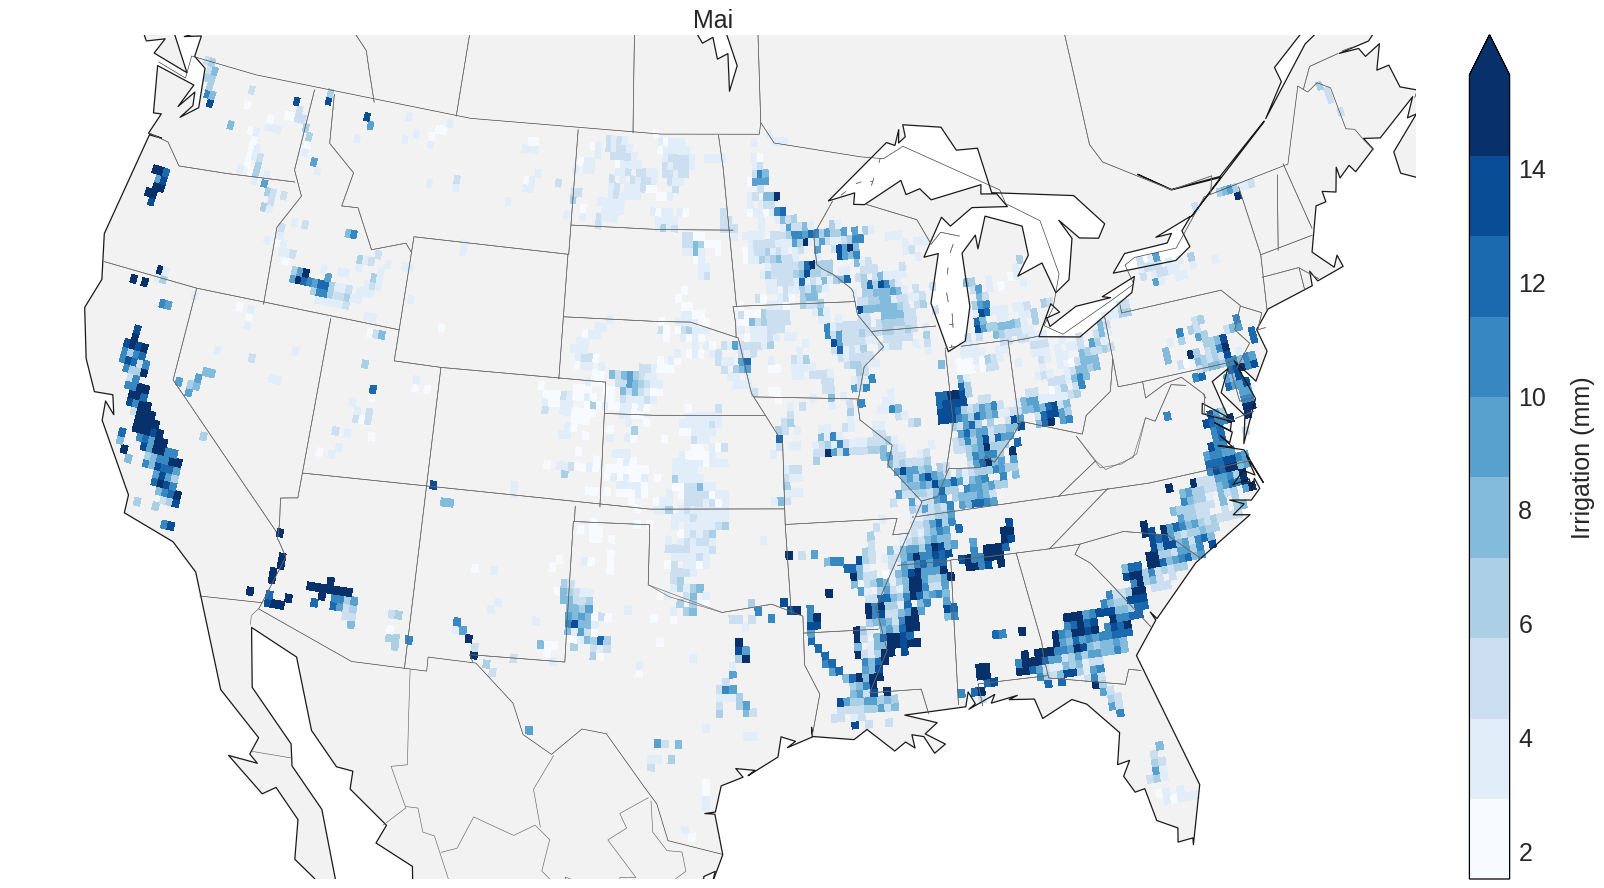
\includegraphics[width=\textwidth]{figures/monthly_clims/ASCAT_monthly_clim_thresh_0_05_Mai}
%    \end{subfigure}
%    \hfill
%    % June
%    \begin{subfigure}[b]{0.3\textwidth}
%        \centering
%        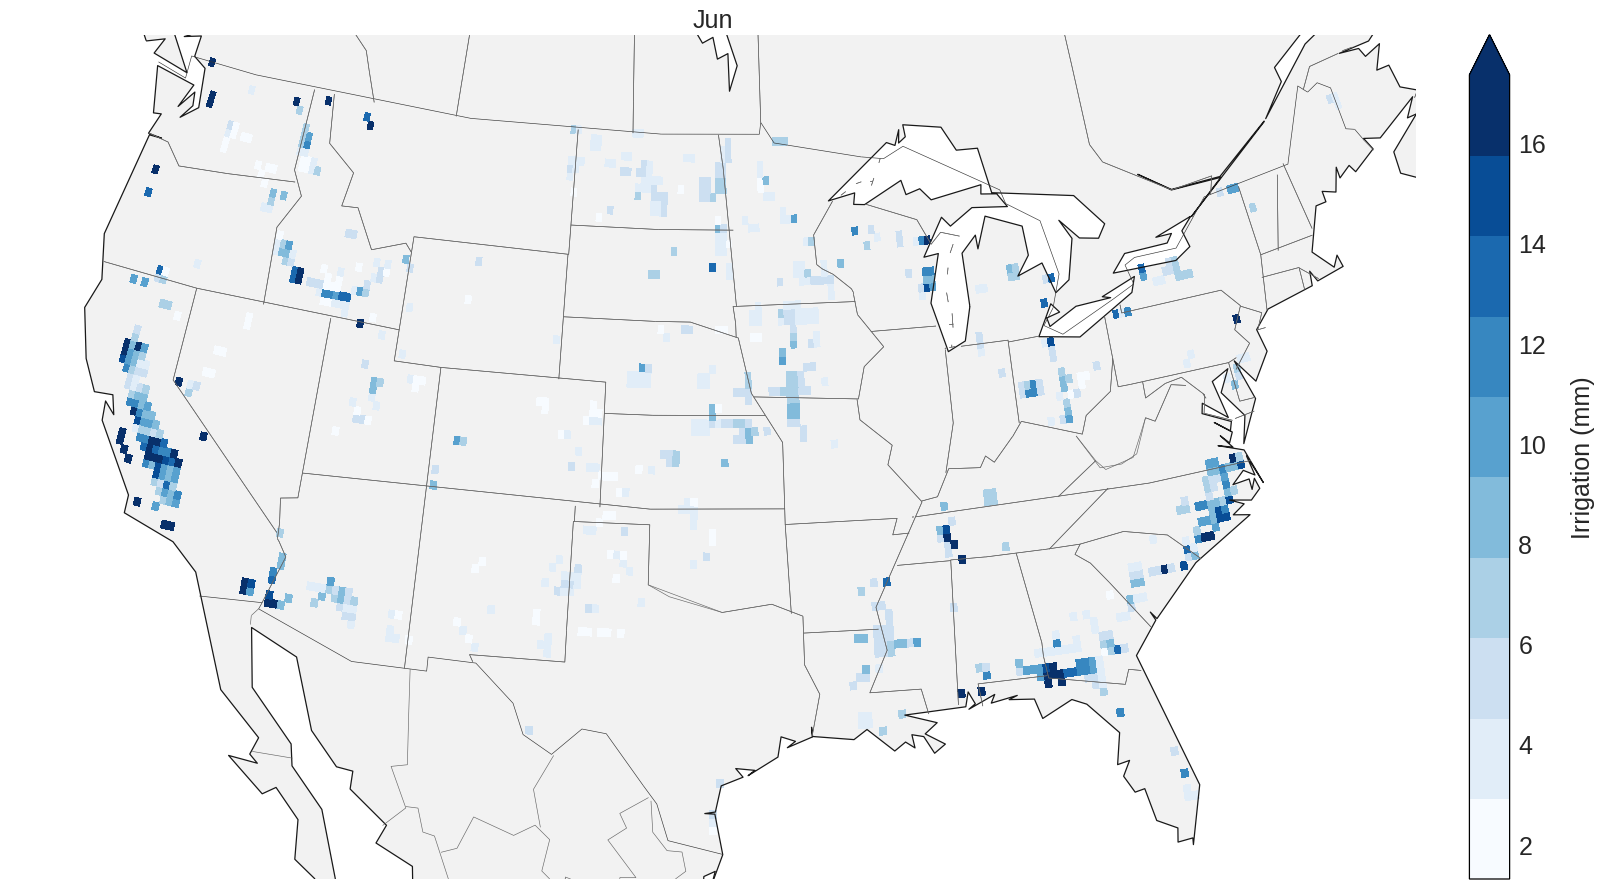
\includegraphics[width=\textwidth]{figures/monthly_clims/SMAP_monthly_clim_thresh_0_05_Jun}
%    \end{subfigure}
%    \hfill
%    \begin{subfigure}[b]{0.3\textwidth}
%        \centering
%        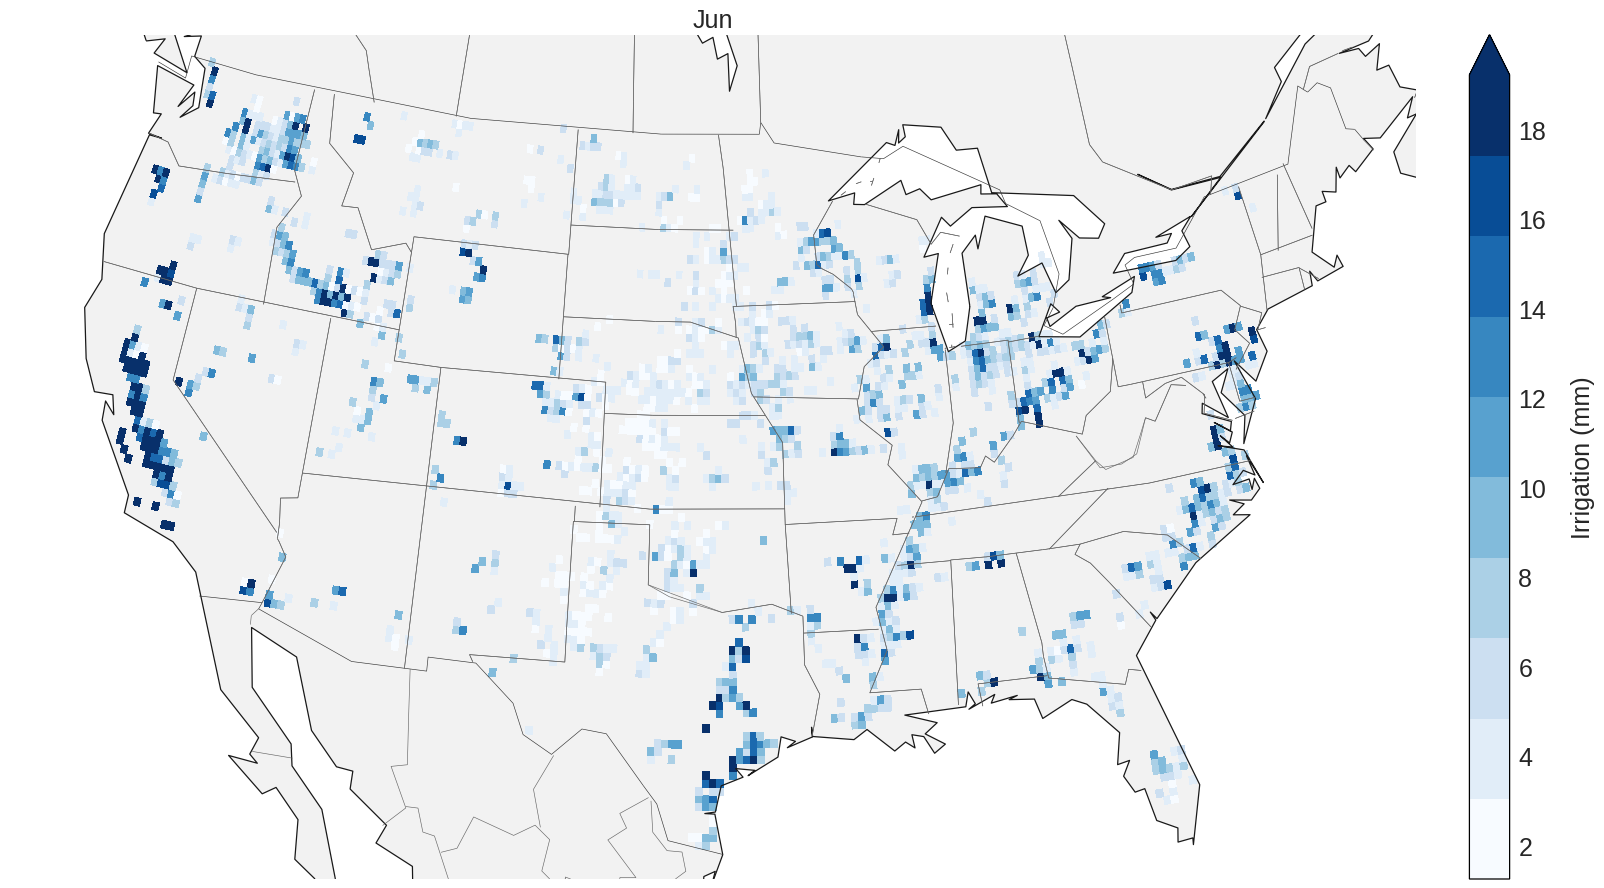
\includegraphics[width=\textwidth]{figures/monthly_clims/AMSR2_monthly_clim_thresh_0_05_Jun}
%    \end{subfigure}
%    \hfill
%    \begin{subfigure}[b]{0.3\textwidth}
%        \centering
%        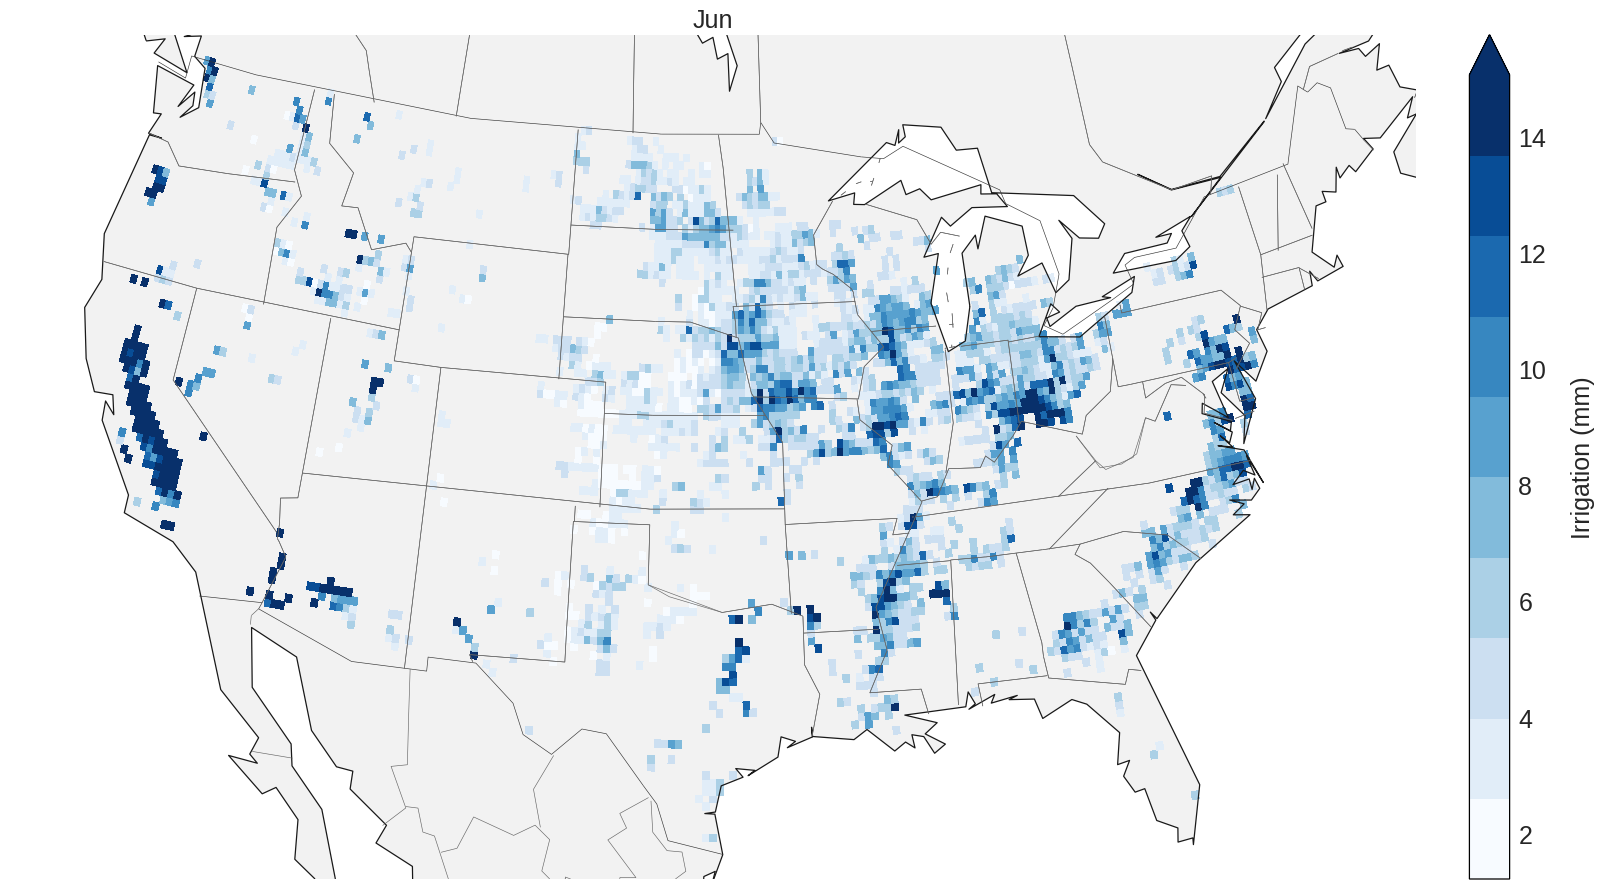
\includegraphics[width=\textwidth]{figures/monthly_clims/ASCAT_monthly_clim_thresh_0_05_Jun}
%    \end{subfigure}
%    \hfill
%    % JULY
%    \begin{subfigure}[b]{0.3\textwidth}
%        \centering
%        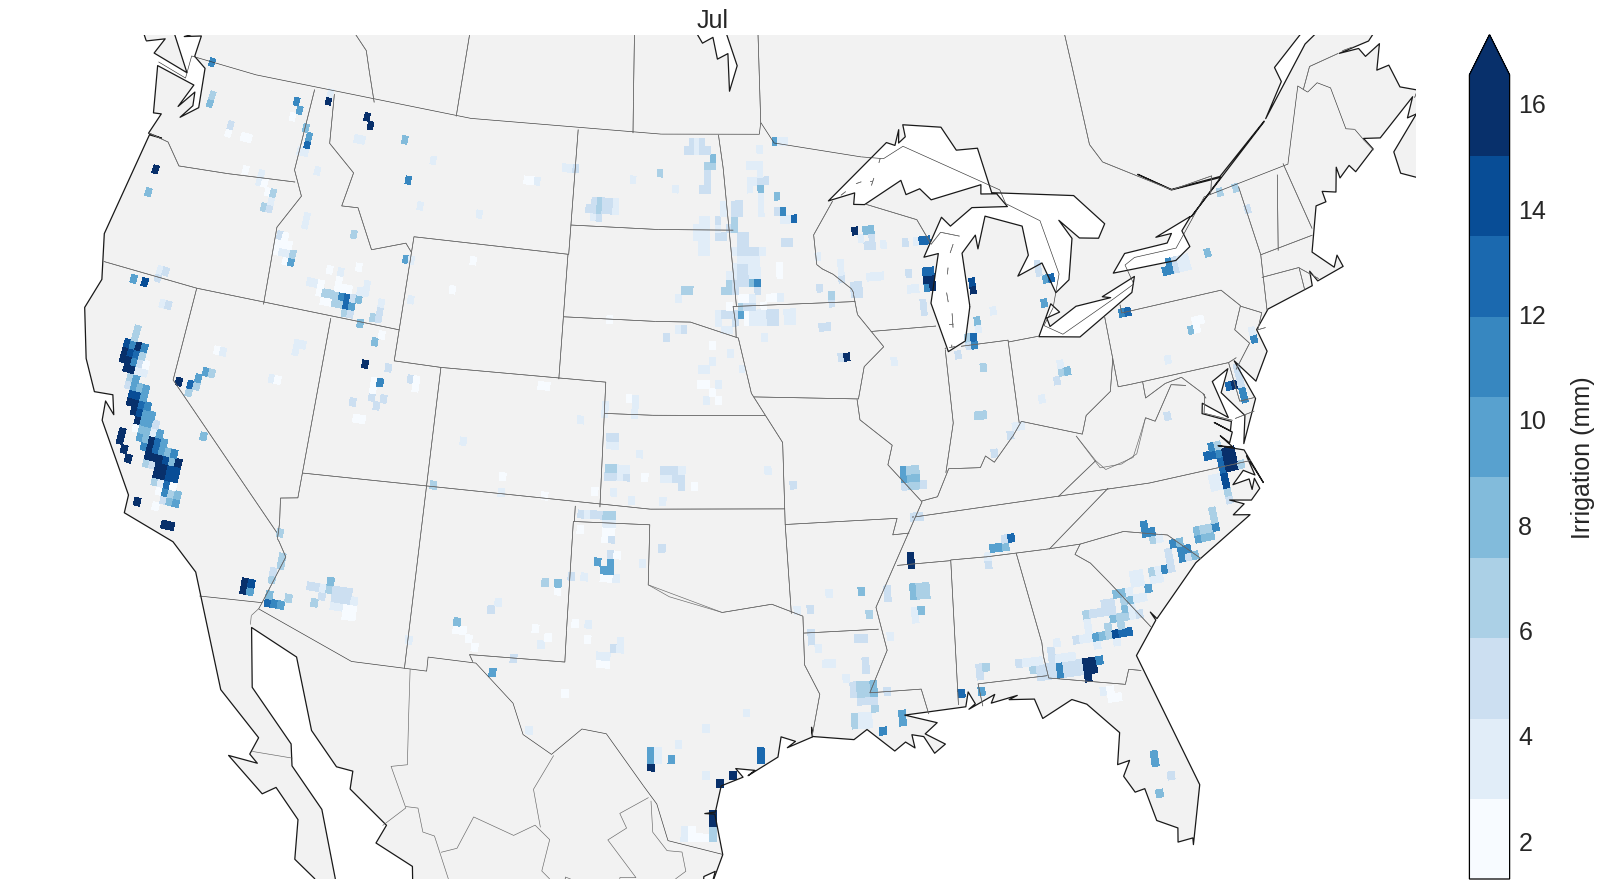
\includegraphics[width=\textwidth]{figures/monthly_clims/SMAP_monthly_clim_thresh_0_05_Jul}
%    \end{subfigure}
%    \hfill
%    \begin{subfigure}[b]{0.3\textwidth}
%        \centering
%        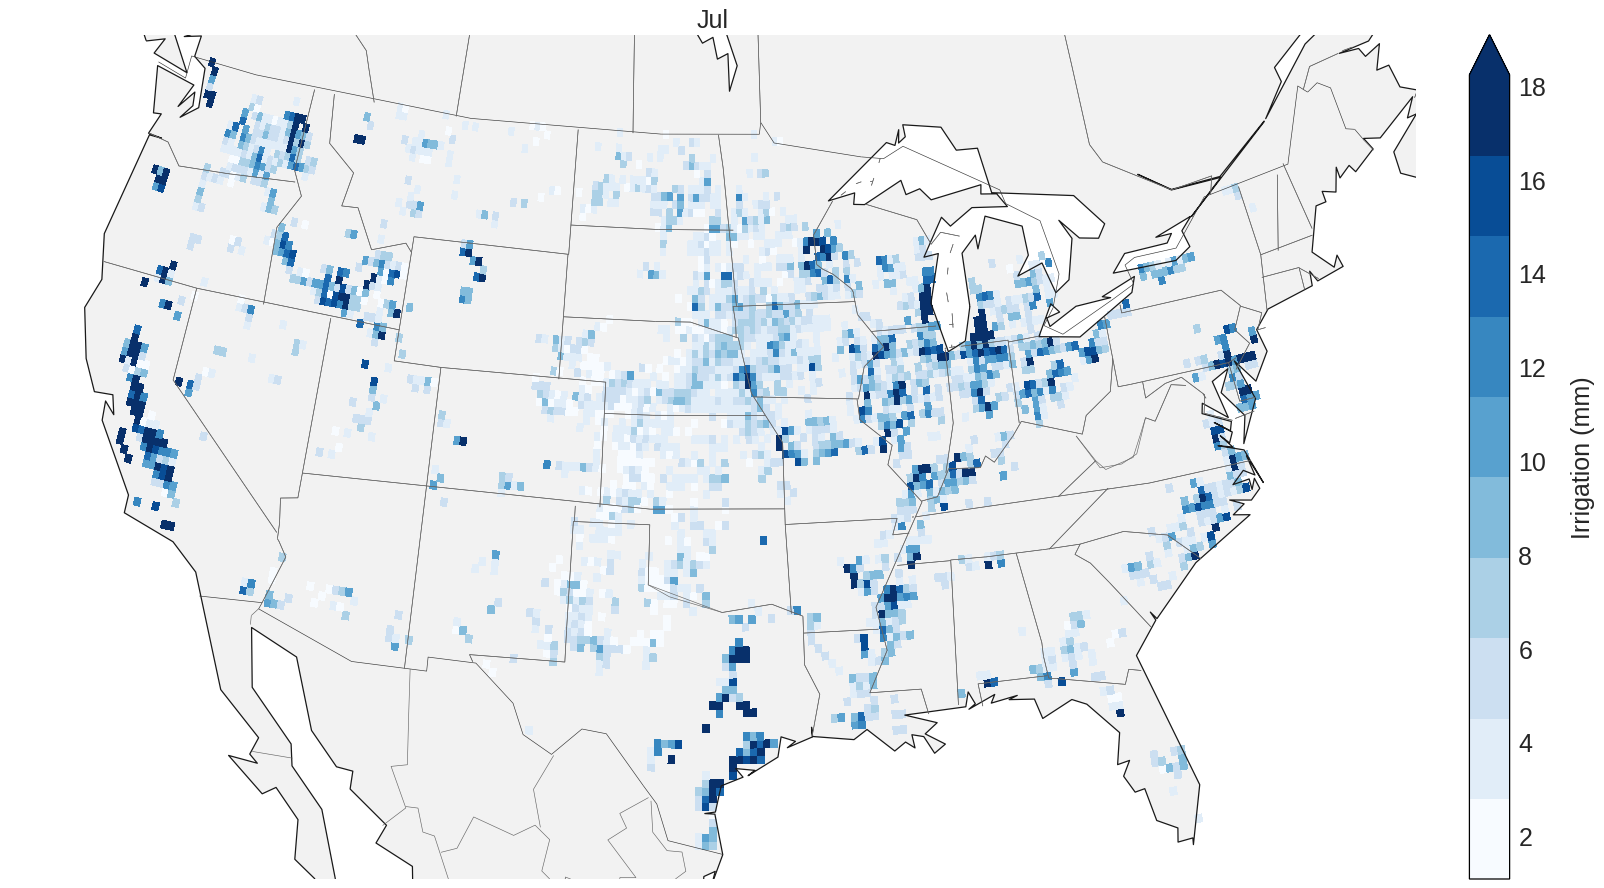
\includegraphics[width=\textwidth]{figures/monthly_clims/AMSR2_monthly_clim_thresh_0_05_Jul}
%    \end{subfigure}
%    \hfill
%    \begin{subfigure}[b]{0.3\textwidth}
%        \centering
%        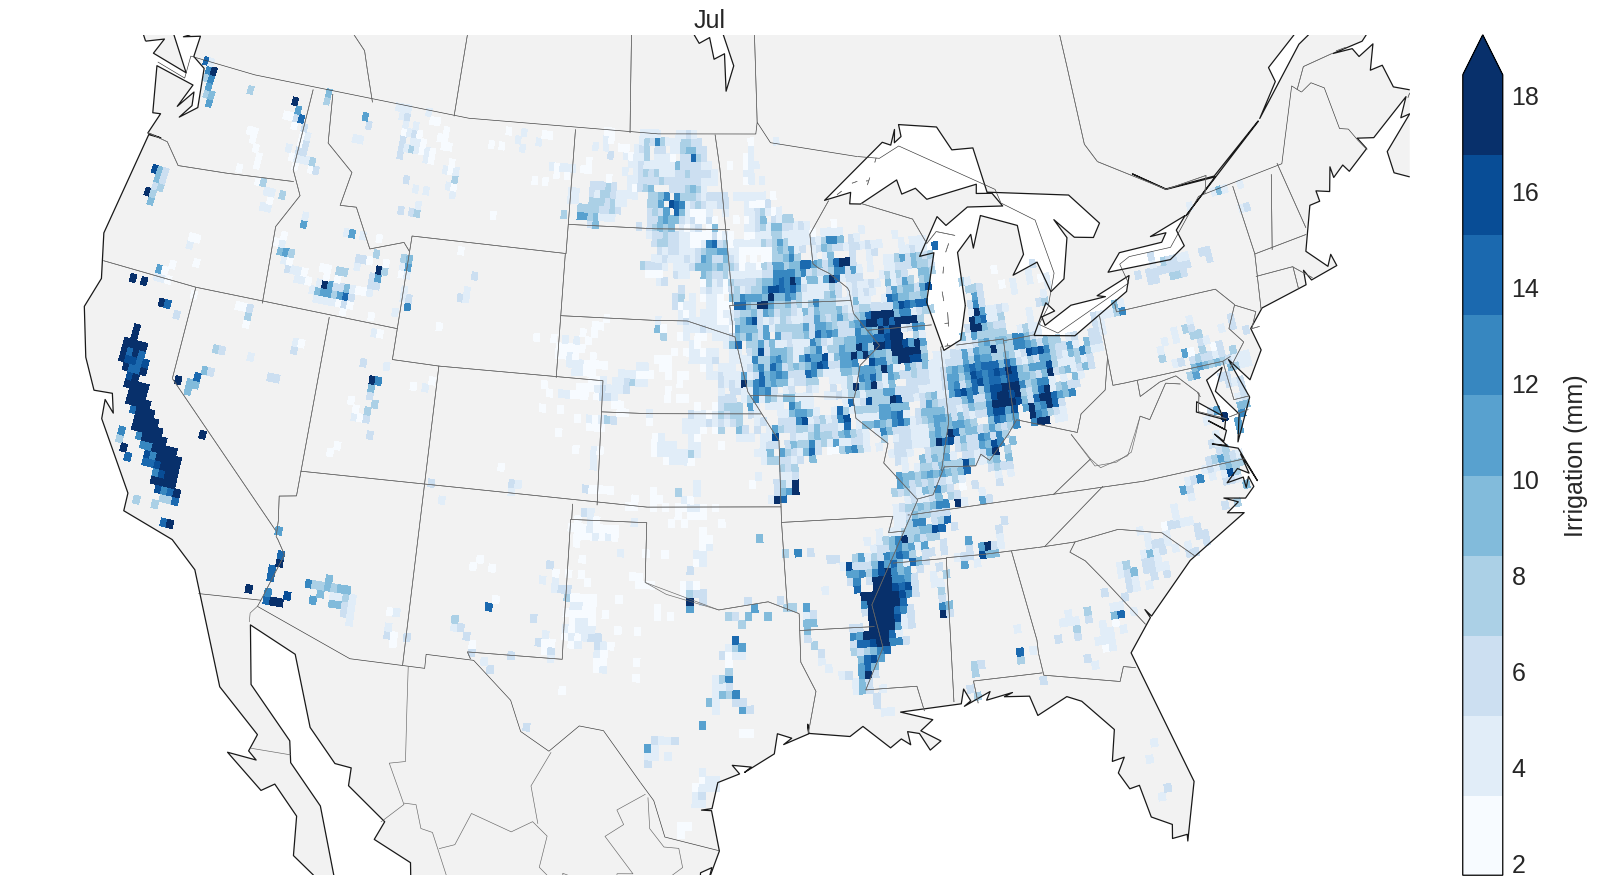
\includegraphics[width=\textwidth]{figures/monthly_clims/ASCAT_monthly_clim_thresh_0_05_Jul}
%    \end{subfigure}
%    \hfill
%    % AUGUST
%    \begin{subfigure}[b]{0.3\textwidth}
%        \centering
%        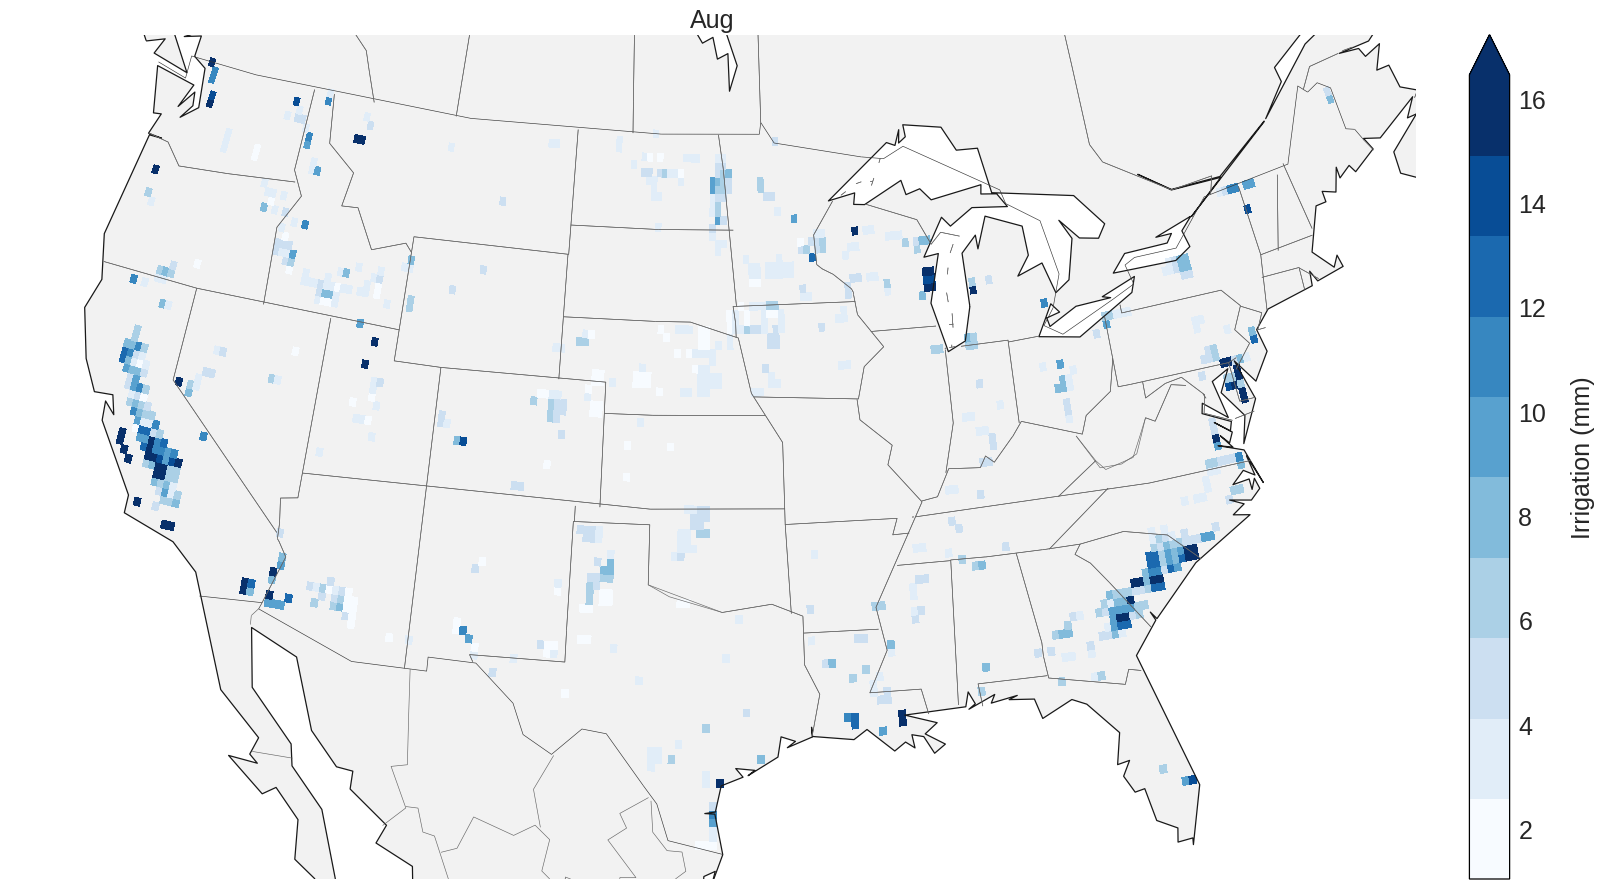
\includegraphics[width=\textwidth]{figures/monthly_clims/SMAP_monthly_clim_thresh_0_05_Aug}
%    \end{subfigure}
%    \hfill
%    \begin{subfigure}[b]{0.3\textwidth}
%        \centering
%        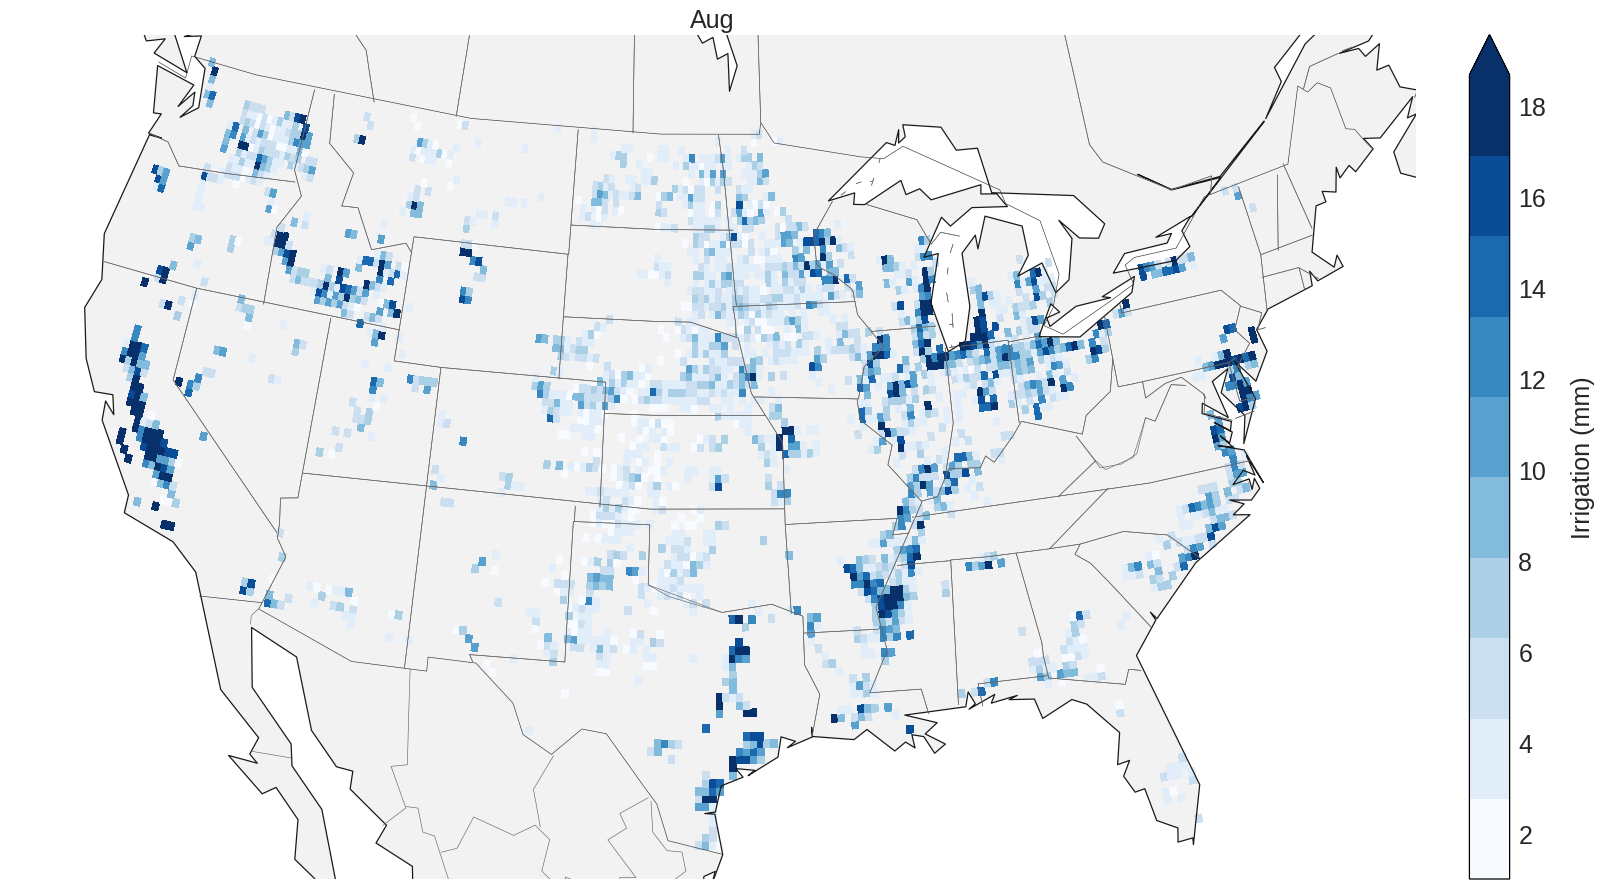
\includegraphics[width=\textwidth]{figures/monthly_clims/AMSR2_monthly_clim_thresh_0_05_Aug}
%    \end{subfigure}
%    \hfill
%    \begin{subfigure}[b]{0.3\textwidth}
%        \centering
%        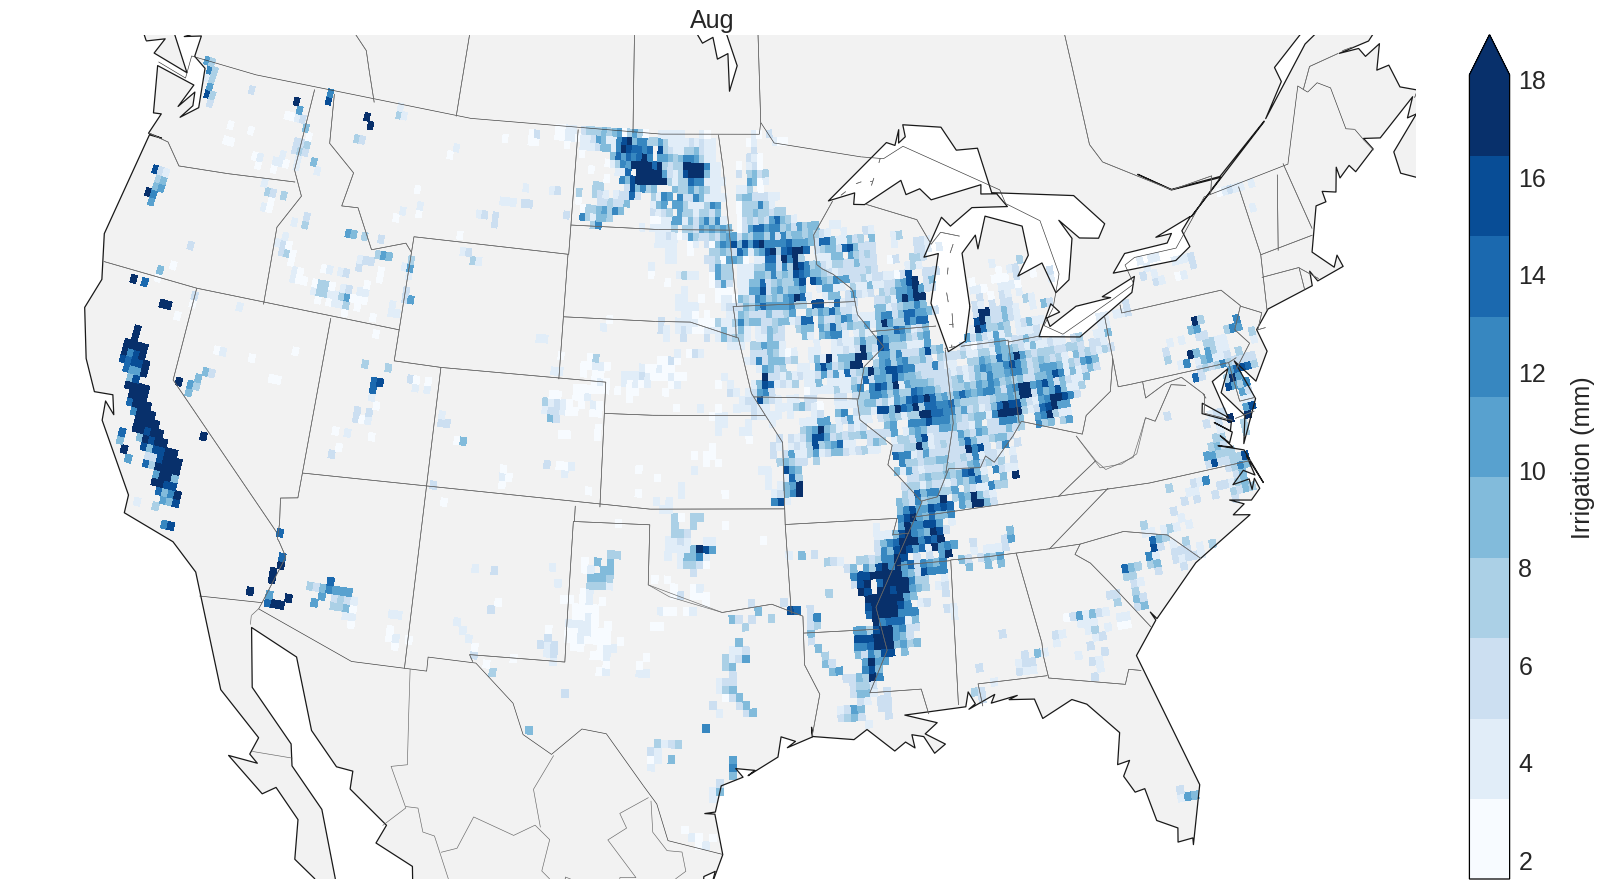
\includegraphics[width=\textwidth]{figures/monthly_clims/ASCAT_monthly_clim_thresh_0_05_Aug}
%    \end{subfigure}
%    \hfill
%    % SEPTEMBER
%    \begin{subfigure}[b]{0.3\textwidth}
%        \centering
%        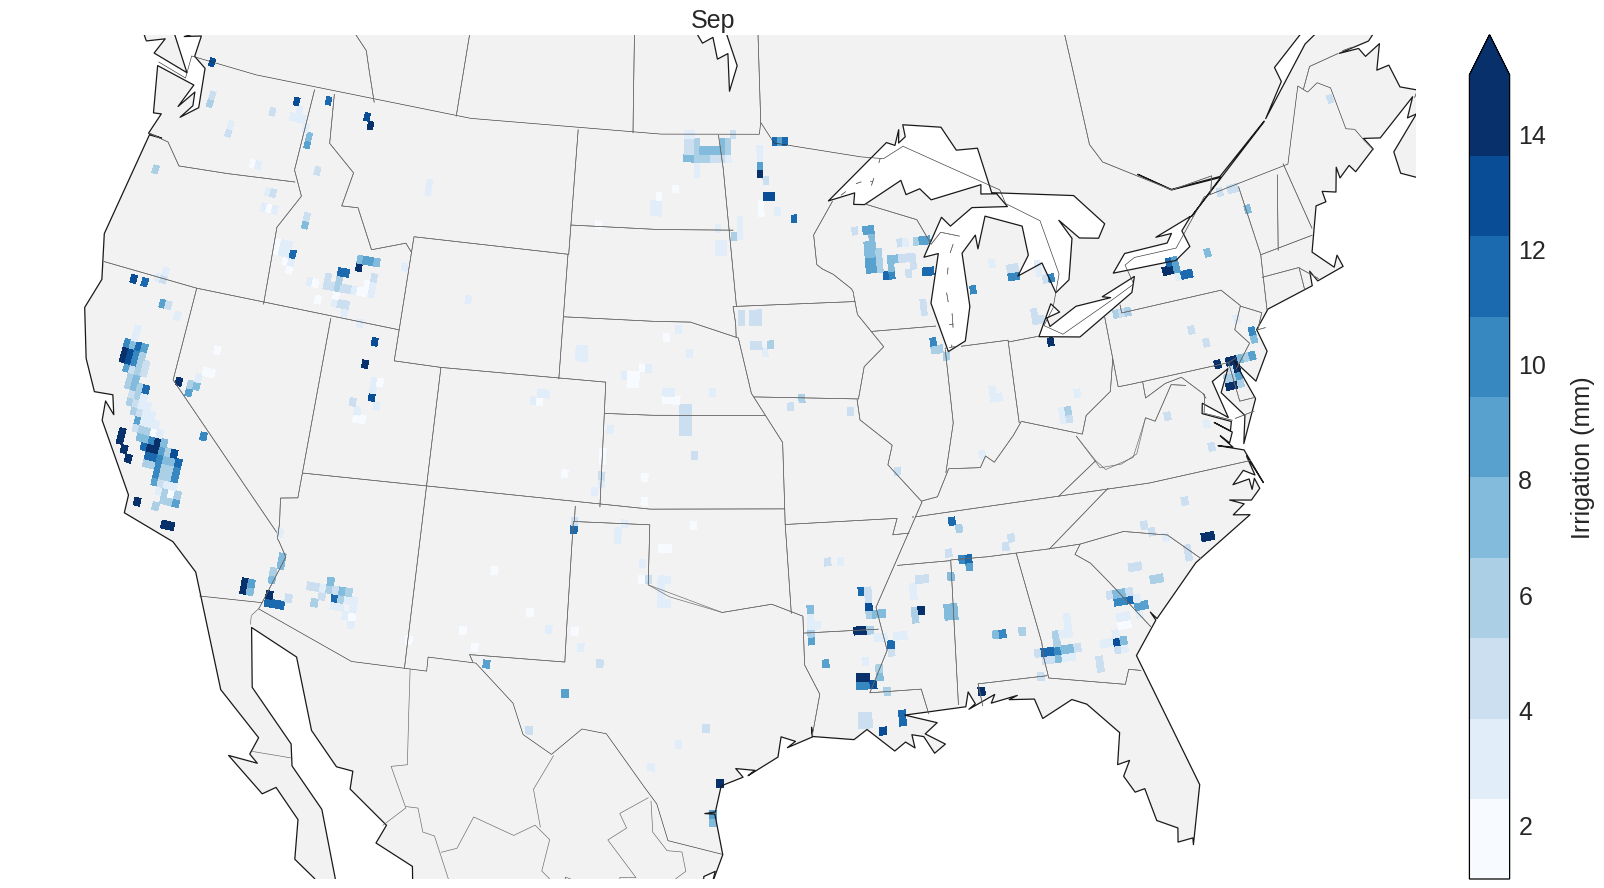
\includegraphics[width=\textwidth]{figures/monthly_clims/SMAP_monthly_clim_thresh_0_05_Sep}
%    \end{subfigure}
%    \hfill
%    \begin{subfigure}[b]{0.3\textwidth}
%        \centering
%        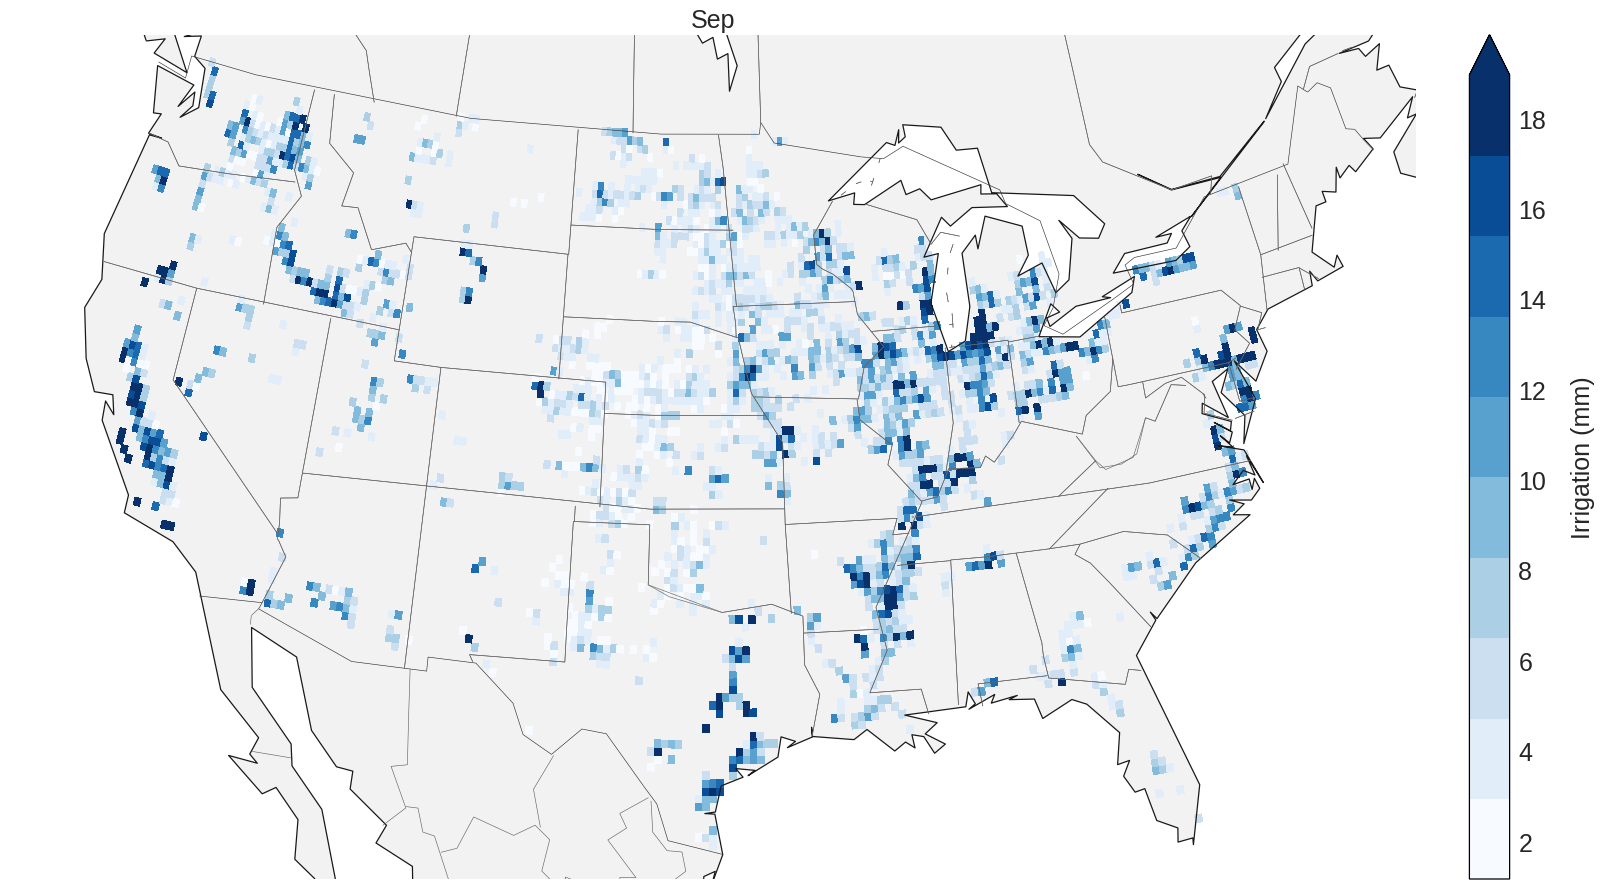
\includegraphics[width=\textwidth]{figures/monthly_clims/AMSR2_monthly_clim_thresh_0_05_Sep}
%    \end{subfigure}
%    \hfill
%    \begin{subfigure}[b]{0.3\textwidth}
%        \centering
%        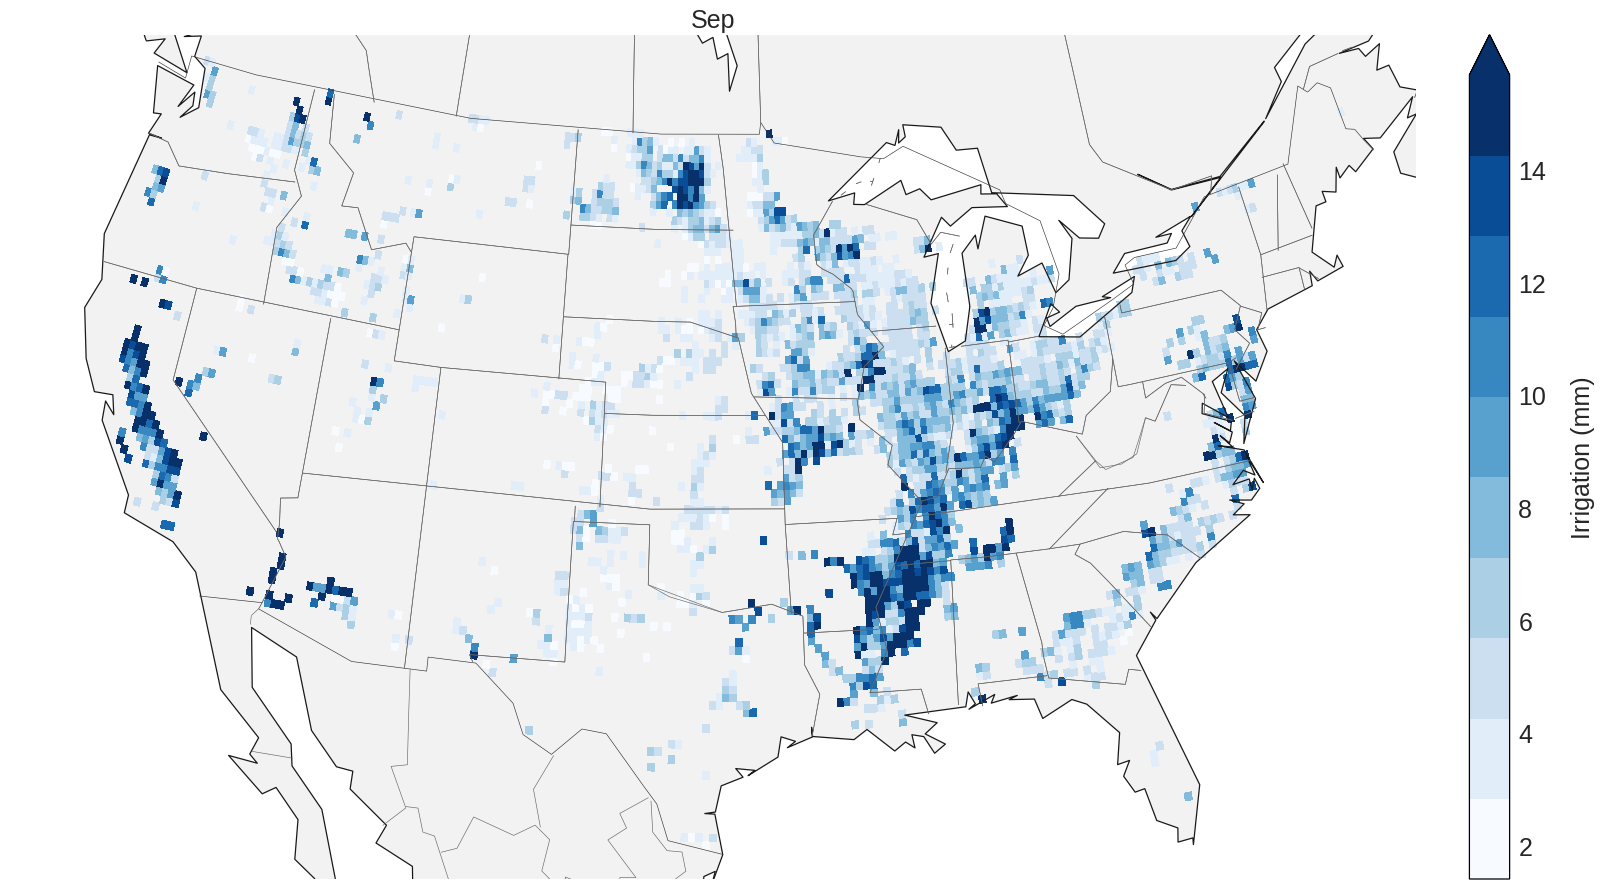
\includegraphics[width=\textwidth]{figures/monthly_clims/ASCAT_monthly_clim_thresh_0_05_Sep}
%    \end{subfigure}
%    \hfill
%    \caption{\textbf{Intra-annual variability of monthly irrigation water use estimates.} The colorbars are binned between 0 and the respective 95th percentiles.}
%    \label{fig:intraannual-variability}
% \end{figure}

\clearpage
% Seasonality of irrigation water use on a state level
\begin{figure}[t]
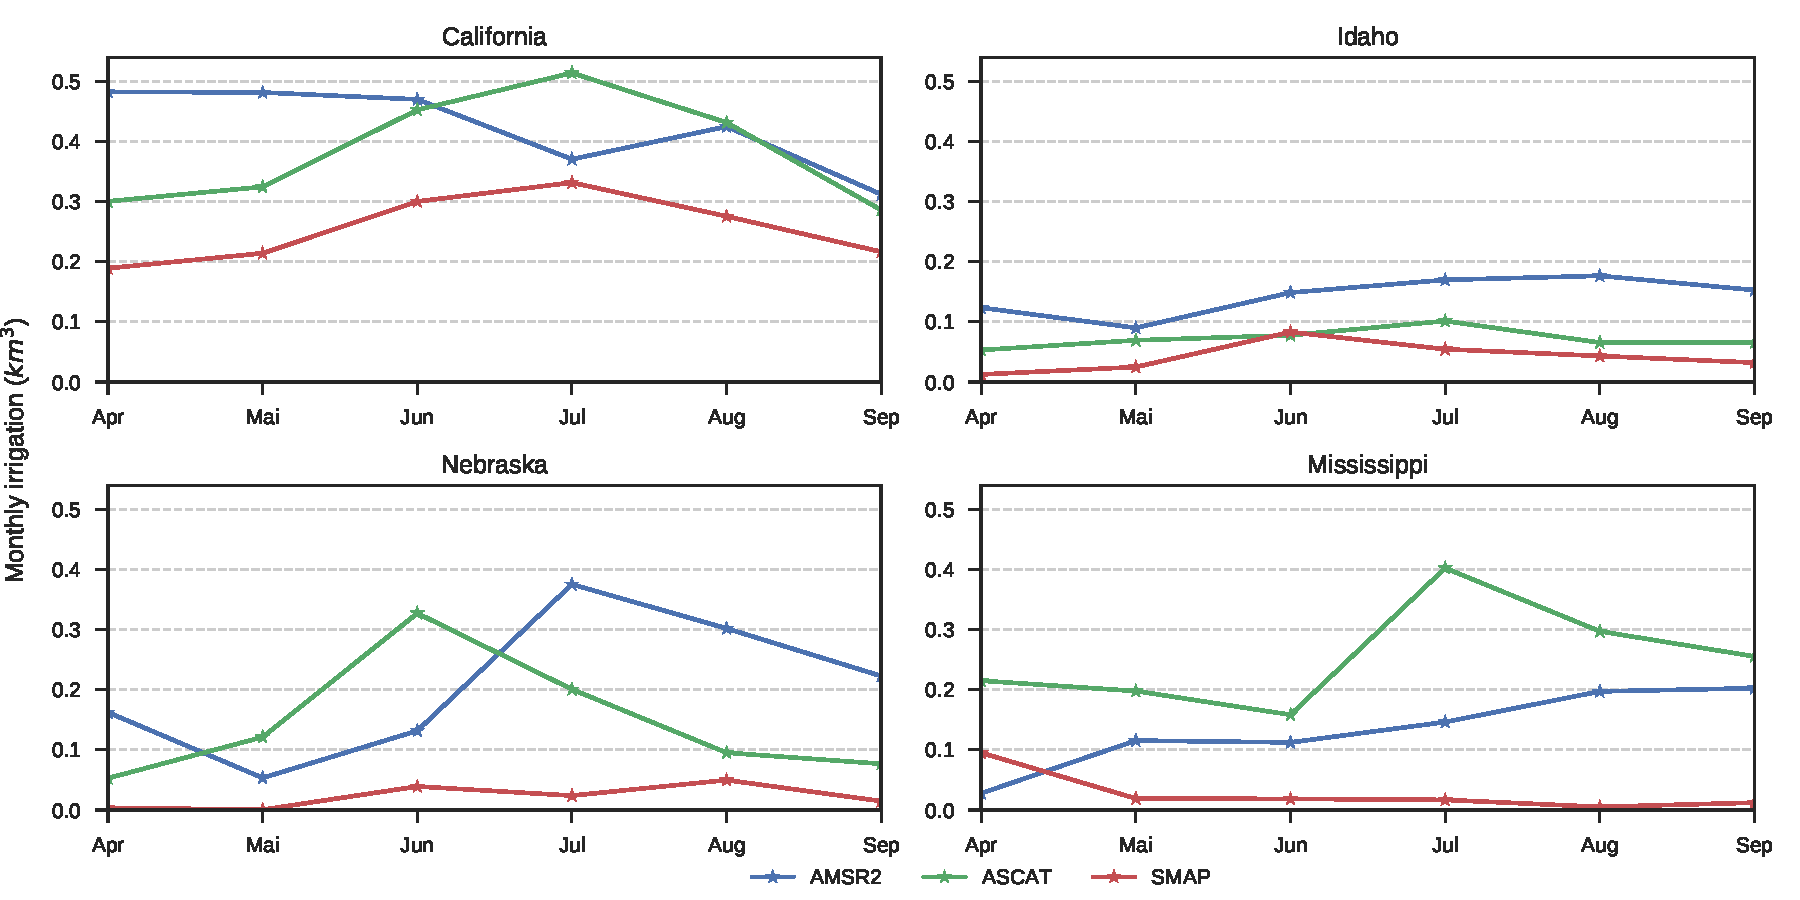
\includegraphics[width=\textwidth]{figures/validation/monthly_water_use_thresh_12}
\caption{\textbf{Seasonality of state-aggregated mean monthly irrigation water use $\overline{IWU}_{M}$ during the growing season.} For each product, the derived $IWU$ at each pixel was multiplied with the corresponding crop fraction to calculate the total irrigation water volume and then aggregated to the state level.}
\label{fig:volume-seasonality}
\end{figure}

%--------------------------------------------------------%
\clearpage
% VALIDATION
\begin{figure}[t]
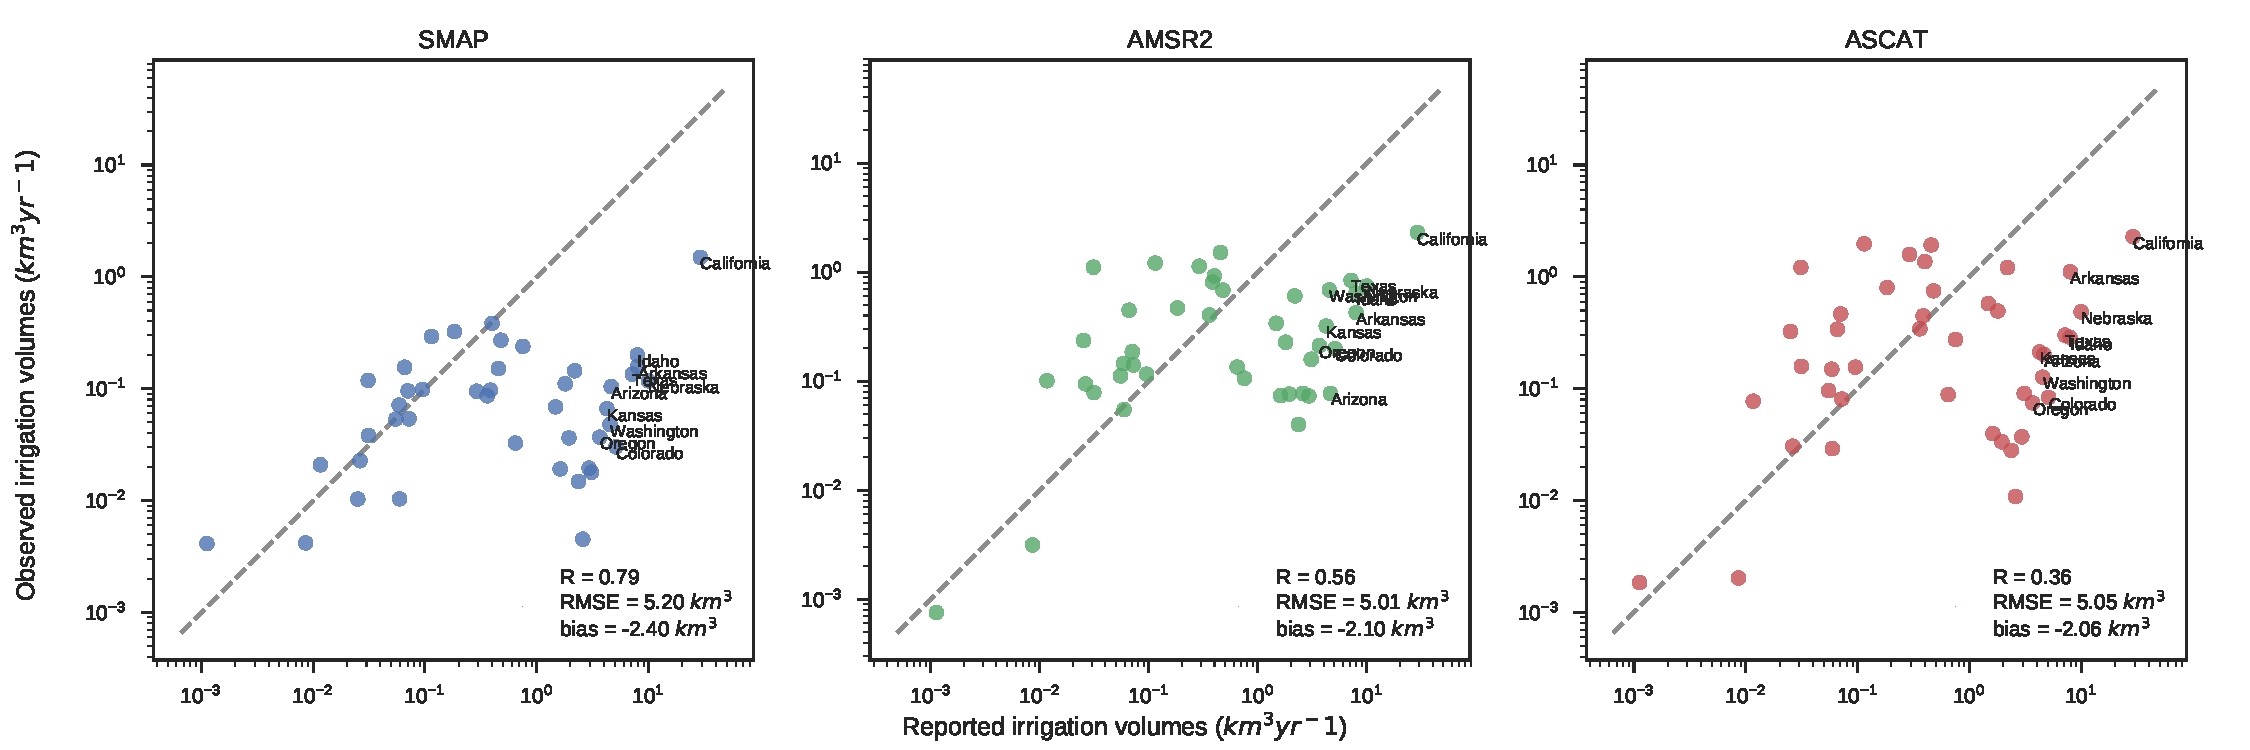
\includegraphics[width=\textwidth]{figures/validation/scatter_plot_states_thresh_12}
\caption{\textbf{Comparison of estimated mean annual irrigation water use and reported irrigation water withdrawals.} For each satellite-model pair, observed $\overline{IWU}_{A}$ was aggregated at the state level. Reported irrigation withdrawals were taken from the 2013 FRIS report and only reflect volumes applied in open fields (e.g. excluding crops grown and irrigated in greenhouses). The data is presented in logarithmic units to reflect both small and large water volumes. Note that the names of the 10 states accounting for the highest irrigation water withdrawals are annotated. $R$, $RMSE$ and $bias$ between observed and reported estimates are shown in the bottom right of each subplot.}
\label{fig:scatter-plot-volumes}
\end{figure}

%--------------------------------------------------------%
%	TABLES
%--------------------------------------------------------%
\clearpage
%%% The different columns must be seperated with a & command and should
%%% end with \\ to identify the column brake.

\begin{table}[t]
\centering
\caption{Data products}
\label{table:data-products}
\begin{tabular}{lllllll}
\hline
\textbf{Data} & \textbf{Product name} & \textbf{\begin{tabular}[c]{@{}l@{}}Data availability/\\ Reference time\end{tabular}} & \textbf{\begin{tabular}[c]{@{}l@{}}Temporal\\ resolution\end{tabular}} & \textbf{\begin{tabular}[c]{@{}l@{}}Spatial\\ resolution\end{tabular}} & \textbf{\begin{tabular}[c]{@{}l@{}}Native\\ gridding\end{tabular}} & \textbf{Units} \\ \hline
SMAP & SMAP\_L3\_v4 & 04/2015 - present & 1-3 days & \textasciitilde 40-km & 36-km & $\si{\cm^{3}.\cm^{-3}}$ \\
AMSR2 & LPRM v06 & 07/2012 - present & 1-2 days & \textasciitilde 25-km & $0.25 \si{\degree}$ & $\si{\m^{3}.\m^{-3}}$ \\
ASCAT & modified H111 & 01/2007 - present & \textasciitilde 1.5 days & \textasciitilde 25-km & 12.5-km & $\%$ \\
MERRA-2 & \begin{tabular}[c]{@{}l@{}}M2T1NXLND.5.12.4 \\ (SFMC parameter)\end{tabular} & 01/1980 - present & \begin{tabular}[c]{@{}l@{}}1 day\\ (resampled)\end{tabular} & \textasciitilde 50-km & $0.625 \si{\degree}$ x $0.5 \si{\degree}$ & $\si{\m^{3}.\m^{-3}}$ \\
\begin{tabular}[c]{@{}l@{}}ESA CCI \\ Land Cover\end{tabular} & LC map 2010 epoch & 2008-2012 & - & \begin{tabular}[c]{@{}l@{}}$0.25 \si{\degree}$\\ (resampled)\end{tabular} & 300-m & - \\
CPC Precipitation & \begin{tabular}[c]{@{}l@{}}Unified Gauge-Based Analysis\\ of Daily Precipitation\end{tabular} & 01/2007 - 12/2016 & 1 day & $0.25 \si{\degree}$ & $0.25 \si{\degree}$ & mm/day \\
MIrAD-US & \begin{tabular}[c]{@{}l@{}}MODIS Irrigated Agriculture\\ Dataset for the United States v3\end{tabular} & 2012 & - & \begin{tabular}[c]{@{}l@{}}$0.25 \si{\degree}$\\ (resampled)\end{tabular} & 250-m & - \\ \hline
\end{tabular}
\end{table}

%--------------------------------------------------------%
\clearpage

\begin{table}[t]
\centering
\caption{\textbf{Sensitivity of different parameter choices within the method on the agreement of estimated $\overline{IWU}_{A}$ with reference irrigation water withdrawals from the 2013 FRIS.} $\frac{d\Theta_{mod}}{dt}$ refers to the masking of precipitation events as inferred from positive model slopes, while $P_{CPC}$ is additional precipitation masking using ancillary CPC data. $T$ is the characteristic time length (days) in the formulation of the exponential filter and  $threshold$ is applied to relative increases in satellite SM $\frac{d\Theta_{sat}}{dt}$ in rain-free periods. Underlined performance scores indicate the best scores within each category, while bold scores show the overall best.}
\label{table:method-evaluation}
\begin{tabular}{@{}lllll@{}}
\toprule
\textbf{Parameter choice} & \textbf{SM product} & \textbf{R} & \textbf{RMSE ($km^{3}$)} & \textbf{bias ($km^{3}$)} \\ \midrule
\multicolumn{5}{c}{Precipitation masking} \\ \midrule
$\frac{d\Theta_{mod}}{dt} = F$ \& $P_{CPC} = F$ & \textit{SMAP} & 0.15 & 5.02 & -0.94 \\
\textbf{} & \textit{AMSR2} & 0.09 & 5.07 & -0.64 \\
\textbf{} & \textit{ASCAT} & -0.02 & 6.35 & 1.08 \\
$\frac{d\Theta_{mod}}{dt} > 0$ \& $P_{CPC} = F$ & \textit{SMAP} & 0.19 & 4.98 & -1.59 \\
\textbf{} & \textit{AMSR2} & 0.12 & 4.99 & -1.22 \\
\textbf{} & \textit{ASCAT} & 0.02 & 5.34 & {\ul \textbf{-0.33}} \\
$\frac{d\Theta_{mod}}{dt} > 0$ \& $P_{CPC} > 0$ & \textit{SMAP} & {\ul 0.46} & 5.03 & -2.11 \\
\textit{} & \textit{AMSR2} & 0.24 & {\ul \textbf{4.94}} & -1.65 \\
\textit{} & \textit{ASCAT} & 0.12 & 4.99 & -1.17 \\ \midrule
\multicolumn{5}{c}{Exponential Filter (Masking: $\frac{d\Theta_{mod}}{dt} > 0$ \& $P_{CPC} > 0$)} \\ \midrule
$T=1$ & \textit{SMAP} & {\ul 0.45} & 5.18 & -2.27 \\
 & \textit{AMSR2} & 0.25 & {\ul 5.08} & -1.98 \\
\textit{} & \textit{ASCAT} & 0.13 & {\ul 5.08} & {\ul -1.78} \\
$T=2$ & \textit{SMAP} & 0.35 & 5.25 & -2.32 \\
 & \textit{AMSR2} & 0.21 & 5.18 & -2.13 \\
 & \textit{ASCAT} & 0.11 & 5.18 & -2.03 \\
$T=3$ & \textit{SMAP} & 0.27 & 5.28 & -2.33 \\
 & \textit{AMSR2} & 0.16 & 5.23 & -2.19 \\
 & \textit{ASCAT} & 0.09 & 5.22 & -2.11 \\ \midrule
\multicolumn{5}{c}{Relative Threshold (Masking: $\frac{d\Theta_{mod}}{dt} > 0$ \& $P_{CPC} > 0$)} \\ \midrule
$\frac{d\Theta_{sat}}{dt} \geqslant 4\%$ & \textit{SMAP} & 0.65 & 5.09 & -2.26 \\
 & \textit{AMSR2} & 0.35 & {\ul 4.95} & -1.85 \\
 & \textit{ASCAT} & 0.15 & 4.99 & {\ul -1.48} \\
$\frac{d\Theta_{sat}}{dt} \geqslant 8\%$ & \textit{SMAP} & 0.75 & 5.15 & -2.35 \\
 & \textit{AMSR2} & 0.47 & 4.98 & -2.00 \\
 & \textit{ASCAT} & 0.23 & 5.01 & -1.82 \\
$\frac{d\Theta_{sat}}{dt} \geqslant 12\%$ & \textit{SMAP} & {\ul \textbf{0.79}} & 5.2 & -2.4 \\
 & \textit{AMSR2} & 0.56 & 5.01 & -2.1 \\
\textit{} & \textit{ASCAT} & 0.36 & 5.05 & -2.06 \\ \bottomrule
\end{tabular}
\end{table}

%--------------------------------------------------------%
\clearpage

\begin{table}[]
\centering
\caption{\textbf{Accuracy assessment of irrigated area estimates.} For each satellite-model combination a confusion matrix between observed $\overline{IWU}_{A}$ and reference irrigated area from the spatially aggregated 2012 MIrAD-US data set was computed after converting the continuous data to a binary representation (pixels with observed $\overline{IWU}_{A} \geq 20mm$ and reported $A_{irrigated} \geq 5\%$ were respectively assigned to the irrigated classes). Results are shown for the four states selected in the regional analysis and the contiguous US (CONUS). Underlines indicate the best scores within each region, while bold scores show the overall best.}
\label{table:accuracy-assessment}
\begin{tabular}{@{}llllllll@{}}
\toprule
\textbf{Region} & \textbf{\begin{tabular}[c]{@{}l@{}}Satellite SM\\ product\end{tabular}} & \textbf{\begin{tabular}[c]{@{}l@{}}Producer's \\ accuracy (\%)\end{tabular}} & \textbf{\begin{tabular}[c]{@{}l@{}}Error of \\ omission (\%)\end{tabular}} & \textbf{\begin{tabular}[c]{@{}l@{}}User's \\ accuracy (\%)\end{tabular}} & \textbf{\begin{tabular}[c]{@{}l@{}}Error of \\ commission (\%)\end{tabular}} & \textbf{\begin{tabular}[c]{@{}l@{}}Overall \\ accuracy (\%)\end{tabular}} & \textbf{\begin{tabular}[c]{@{}l@{}}Kappa\\ score (-)\end{tabular}} \\ \midrule
California & SMAP & {\ul \textbf{95.06}} & {\ul 4.94} & {\ul \textbf{78.57}} & {\ul 21.43} & {\ul \textbf{77.68}} & {\ul \textbf{0.33}} \\
 & AMSR2 & 87.65 & 12.35 & 73.96 & 26.04 & 68.75 & 0.08 \\
 & ASCAT & {\ul \textbf{95.06}} & {\ul 4.94} & 75.49 & 24.51 & 74.11 & 0.18 \\ \midrule
Idaho & SMAP & 9.84 & 90.16 & {\ul 54.54} & 45.45 & 50.82 & 0.02 \\
 & AMSR2 & {\ul 59.02} & {\ul 40.98} & 59.02 & 40.98 & {\ul 59.02} & {\ul 0.18} \\
 & ASCAT & 22.95 & 77.05 & 60.87 & {\ul 39.13} & 54.1 & 0.08 \\ \midrule
Nebraska & SMAP & 0 & 100 & 0 & {\ul \textbf{0}} & 19.01 & {\ul 0} \\
 & AMSR2 & {\ul 4.08} & {\ul 95.92} & {\ul 57.14} & 42.86 & {\ul 19.83} & -0.04 \\
 & ASCAT & 0.51 & 99.49 & 50 & 50 & 19.01 & -0.01 \\ \midrule
Mississippi & SMAP & 0 & 100 & 0 & 100 & 60 & -0.11 \\
 & AMSR2 & 45.16 & 54.84 & {\ul 60.87} & {\ul 39.13} & {\ul 71.11} & {\ul 0.32} \\
 & ASCAT & {\ul 100} & {\ul \textbf{0}} & 37.35 & 62.65 & 42.22 & 0.08 \\ \midrule
CONUS & SMAP & 9.95 & 90.05 & {\ul 46.36} & {\ul 53.64} & {\ul 74.03} & {\ul 0.08} \\
 & AMSR2 & {\ul 27.30} & {\ul 72.7} & 32.36 & 67.64 & 66.82 & {\ul 0.08} \\
 & ASCAT & 25.25 & 74.75 & 25.35 & 74.65 & 61.88 & 0 \\ \bottomrule
\end{tabular}
\end{table}

%--------------------------------------------------------%
%	TEMPLATES
%--------------------------------------------------------%
%% ONE-COLUMN FIGURES

%%f
%\begin{figure}[t]
%\includegraphics[width=8.3cm]{FILE NAME}
%\caption{TEXT}
%\end{figure}
%
%%% TWO-COLUMN FIGURES
%
%%f
% \begin{figure}[t]
% \includegraphics[width=12cm]{FILE NAME}
% \caption{TEXT}
% \end{figure}
%
%
%%% ONE-COLUMN TABLE
%
%%t
%\begin{table}[t]
%\caption{TEXT}
%\begin{tabular}{column = lcr}
%\tophline
%
%\middlehline
%
%\bottomhline
%\end{tabular}
%\belowtable{} % Table Footnotes
%\end{table}
%
%%% TWO-COLUMN TABLE
%
%%t
%\begin{table*}[t]
%\caption{TEXT}
%\begin{tabular}{column = lcr}
%\tophline
%
%\middlehline
%
%\bottomhline
%\end{tabular}
%\belowtable{} % Table Footnotes
%\end{table*}
%
%%% LANDSCAPE TABLE
%
%%t
%\begin{sidewaystable*}[t]
%\caption{TEXT}
%\begin{tabular}{column = lcr}
%\tophline
%
%\middlehline
%
%\bottomhline
%\end{tabular}
%\belowtable{} % Table Footnotes
%\end{sidewaystable*}
%
%
%%% MATHEMATICAL EXPRESSIONS
%
%%% All papers typeset by Copernicus Publications follow the math typesetting regulations
%%% given by the IUPAC Green Book (IUPAC: Quantities, Units and Symbols in Physical Chemistry,
%%% 2nd Edn., Blackwell Science, available at: http://old.iupac.org/publications/books/gbook/green_book_2ed.pdf, 1993).
%%%
%%% Physical quantities/variables are typeset in italic font (t for time, T for Temperature)
%%% Indices which are not defined are typeset in italic font (x, y, z, a, b, c)
%%% Items/objects which are defined are typeset in roman font (Car A, Car B)
%%% Descriptions/specifications which are defined by itself are typeset in roman font (abs, rel, ref, tot, net, ice)
%%% Abbreviations from 2 letters are typeset in roman font (RH, LAI)
%%% Vectors are identified in bold italic font using \vec{x}
%%% Matrices are identified in bold roman font
%%% Multiplication signs are typeset using the LaTeX commands \times (for vector products, grids, and exponential notations) or \cdot
%%% The character * should not be applied as mutliplication sign

\end{document}